\documentclass[10pt]{article}

\usepackage{a4wide}
\usepackage{amsmath}
\usepackage{amssymb}
\usepackage{amsfonts}
\usepackage{braket}
\usepackage{todonotes}
\usepackage{bbold}
\usepackage{multicol}
\usepackage{dsfont}
%\usepackage[bookmarks,colorlinks=true,linkcolor=blue,urlcolor=black,bookmarksopen=true,bookmarksdepth=2]{hyperref}
\usepackage[bookmarks]{hyperref}
\setlength{\parindent}{0pt}

\def\threej#1{\inthreej(#1)}
\def\inthreej(#1,#2,#3,#4,#5,#6){\begin{pmatrix}#1 & #2 & #3 \\ #4 & #5 & #6 \end{pmatrix}}

\def\cgcthreej#1{\incgcthreej(#1)}
\def\incgcthreej(#1,#2,#3,#4,#5,#6){ (-1)^{#1-#2+#6} \sqrt{ 2 #3 + 1 } \begin{pmatrix}#1 & #2 & #3 \\ #4 & #5 & -#6 \end{pmatrix}}

\def\sixj#1{\insixj(#1)}
\def\insixj(#1,#2,#3,#4,#5,#6){\begin{Bmatrix}#1 & #2 & #3 \\ #4 & #5 & #6 \end{Bmatrix}} 

\begin{document}


\rule{\textwidth}{2pt} \\ [-0.8\baselineskip]
\rule{\textwidth}{1pt}
\begin{center}
{\Huge \textsc{LCA CODE MANUAL}} \\
\vspace{10pt}
\textsc{ -- Camille Colle -- }
\end{center}
\rule{\textwidth}{1pt} \\ [-0.75\baselineskip]
\rule{\textwidth}{2pt} \\ [2\baselineskip]

\tableofcontents

\section{Code tipz}
Maartens code contains a lot of ``prints''' so your the output of the test program may be difficult to isolate.
A possible solution is to use a makeshift filter in the following way. Tag your prints with a marker, for example \texttt{std::cout << "[mymarker] ... " << std::endl;}. When you run your program, you can use something like \texttt{./myprogram | tee fulloutput.log | grep "\textasciicircum[mymarker]" }.
The file \texttt{fulloutput.log} will contain the full output.

\section{Definitions}
\label{sec:def}
A short (probably incomplete) overview of the quantities used in this manual,
$\psi_{n l m_{l}} (\vec{r})$ are the $\vec{r}$-space solutions of the harmonic oscillator with parameter $\nu = m_{N} \omega / \hbar $,
\begin{align}
\psi_{n l m_{l}}(\vec{r}) &= R_{n l} (r) Y_{l m}(\Omega_{r}) \, , \\
R_{n l}(r) &= \left[ \frac{ 2n!}{\Gamma(n+l+\frac{3}{2})} \nu^{l+\frac{3}{2}} \right]^{\frac{1}{2}} r^{l} e^{-\frac{\nu r^{2}}{2}} L_{n}^{l+\frac{1}{2}}( \nu r^{2}) \, .
\end{align}
$m_N$ is the average nucleon mass, $938.5$ MeV (this appears to be $938.0$ in the code).
$\hbar \omega$ is parameterized as,
\begin{align}
	\hbar \omega = 45 A^{-\frac{1}{3}} - 25 A^{-\frac{2}{3}} \, [\text{MeV}] .
\end{align}
$\nu$ in function of the mass number $A$ is displayed in figure~\ref{fig:Adepnu}.
\begin{figure}
\centering
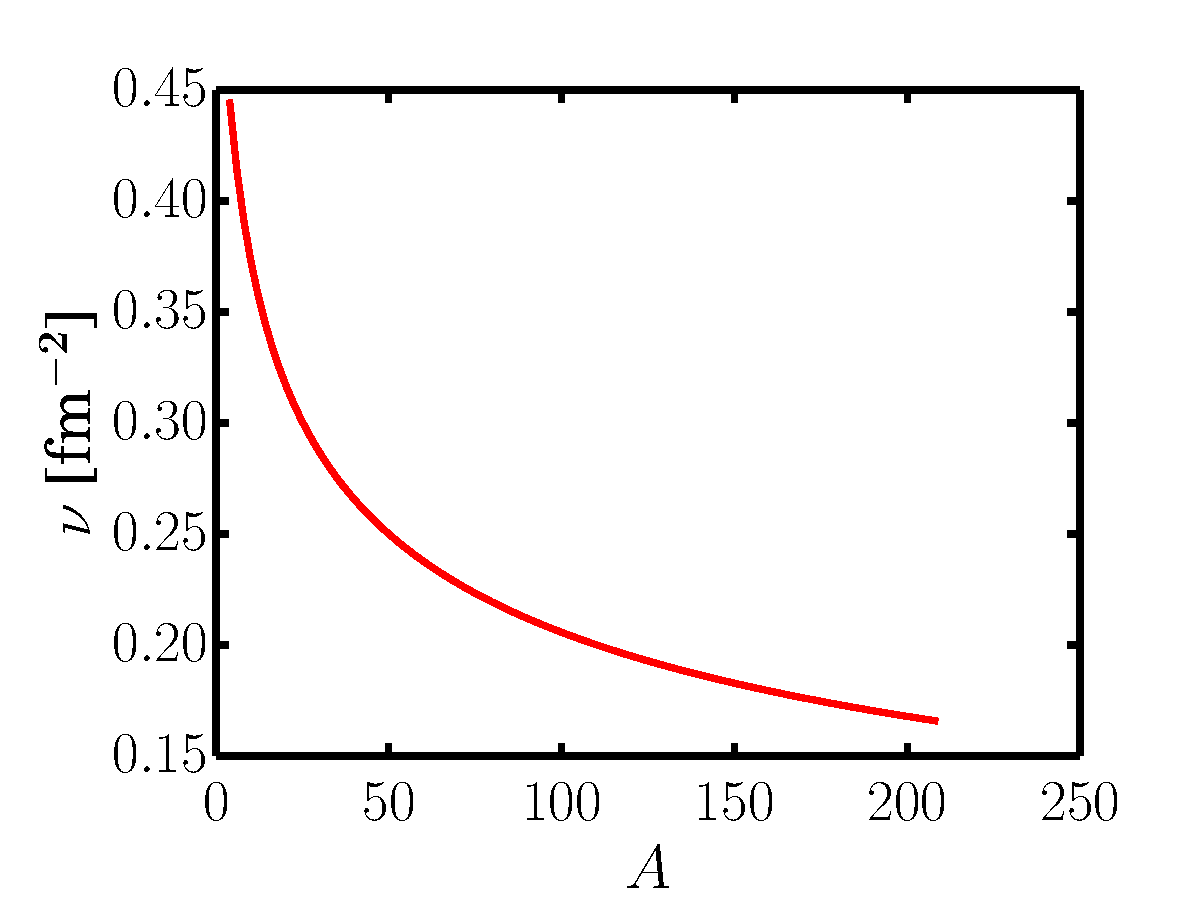
\includegraphics[width=0.7\textwidth]{figures/Adepnu.pdf}
\caption{The harmonic-oscillator parameter $\nu$ in function of the mass number $A$.}
\label{fig:Adepnu}
\end{figure}
It is well known that the solutions $\phi_{n l m_{l}} (\vec{p})$  in $\vec{p}$-space are of the exact same form, where compared to the $\vec{r}$-space solution $\vec{r}$ is replaced by $\vec{p}$ and $\nu$ by $\nu' = 1/\nu$.
However, when taking the explicit Fourier transformation, some (non-neglectable) phase factors appear (see Sec.~\ref{sec:ft_transforms}),
\begin{align}
	\phi_{n l m_{l}}(\vec{p}) &= \frac{1}{(2\pi)^{ \frac{3}{2}}}  \int \text{d}^{3} \vec{r} e^{- i \vec{p} \cdot \vec{r}} \psi_{n l m_{l}}(\vec{r}) \\
	&= i^{-l} (-1)^{n} \left[ \frac{ 2n!}{\Gamma(n+l+\frac{3}{2})} \nu'^{l+\frac{3}{2}} \right]^{\frac{1}{2}} p^{l} e^{-\frac{\nu' p^{2}}{2}} L_{n}^{l+\frac{1}{2}}(\nu'p^{2})  Y_{l m}(\Omega_p) \\
	&= i^{-l} (-1)^{n} \Pi_{n l}(p)  Y_{l m}(\Omega_p) \, , \\
 \Pi_{n l}(p) &= \left[ \frac{ 2n!}{\Gamma(n+l+\frac{3}{2})} \nu'^{l+\frac{3}{2}} \right]^{\frac{1}{2}} p^{l} e^{-\frac{\nu' p^{2}}{2}} L_{n}^{l+\frac{1}{2}}(\nu'p^{2})
\end{align}
Here, the Laguerre polynomials are often expanded as follows,
\begin{align}
	L_{n}^{l+\frac{1}{2}}(x) &= \sum_{i=0}^{n} a_{nl,i} x^{i} \, , \notag \\
	a_{nl,i} &= (-1)^{i} \frac{ \Gamma(n+l+3/2) }{ \Gamma(i+l+3/2)(n-i)! i!}
	\label{eq:def:laguerre_exp}
\end{align}
In the LCA a one-body operator $\widehat{\Omega}^{[1]} = \sum_{i}^{A} \widehat{\Omega}_{i}$ becomes,
\begin{equation}
	\widehat{\Omega}^{[1],\,\text{LCA}} = \widehat{\Omega}^{[1]} + \sum_{i,j \neq i}^{A} \left( \hat{l}_{ij}^{\dagger} \widehat{\Omega}_{i} +  \widehat{\Omega}_{i} \hat{l}_{ij} + \hat{l}_{ij}^{\dagger}  \widehat{\Omega}_{i} \hat{l}_{ij} \right) \, .
	\label{eq:LCA_one_body}
\end{equation}
In similar vein, the LCA transforms a two-body operator $\widehat{\Omega}^{[2]} = \sum_{i<j} \widehat{\Omega}_{ij}$ to,
\begin{multline}
	\widehat{\Omega}^{[2],\,\text{LCA}} = 
	\widehat{\Omega}^{[2]}
	+ \sum_{m<n}^{A} \sum_{i<j}^{A} \left(
		\hat{l}_{mn}^{\dagger} \widehat{\Omega}_{ij} +
		\widehat{\Omega}_{ij} \hat{l}_{mn} +
		\hat{l}_{mn}^{\dagger} \widehat{\Omega}_{ij} \hat{l}_{mn}
	\right) \\ 
	\times \left[ ( \delta_{mi} + \delta_{ni} + \delta_{mj} + \delta_{nj} ) ( 1 - \delta_{mi} \delta_{nj})( 1 - \delta_{mj} \delta_{ni}) + \delta_{mi} \delta_{nj} + \delta_{mj} \delta_{ni} \right] \\
	= \widehat{\Omega}^{[2]} + 
	\sum_{i<j}^{A} \Big[ 
	\hat{l}_{ij}^{\dagger} \widehat{\Omega}_{ij} +
	\widehat{\Omega}_{ij} \hat{l}_{ij} +
	\hat{l}_{ij}^{\dagger} \widehat{\Omega}_{ij} \hat{l}_{ij} \\
	+ \sum_{n \notin \{i,j\}}^{A} 
	(\hat{l}_{in}^{\dagger} + \hat{l}_{jn}^{\dagger} ) \widehat{\Omega}_{ij} +
	\widehat{\Omega}_{ij} (\hat{l}_{in} + \hat{l}_{jn}) + 
	\hat{l}_{in}^{\dagger} \widehat{\Omega}_{ij} \hat{l}_{in} + \hat{l}_{jn}^{\dagger} \widehat{\Omega}_{ij} \hat{l}_{jn} 
	 \Big] \, .
	 \label{eq:LCA_two_body}
\end{multline} 

To preserve normalization the normalisation denominator $ \mathcal{N} = \braket{ \Phi | \widehat{\mathcal{G}}{^\dagger} \mathcal{G} | \Phi }$, should be expanded to the same order in $\hat{l}$ as the numerator. The normalisation factor $\mathcal{N}$ can be calculated by replacing $\widehat{\Omega}_i$ with $\frac{1}{A}$ in Eq.~(\ref{eq:LCA_one_body}) or $\widehat{\Omega}_{ij}$ with $\frac{2}{A(A-1)}$ in Eq.~(\ref{eq:LCA_two_body}),
\begin{align}
	\mathcal{N}^{[1]} &=  1 + \frac{2}{A} \sum_{i < j}^{A} \braket{ \alpha_{i} \alpha_{j} | \hat{l}^{\dagger}_{ij} + \hat{l}_{ij} + \hat{l}^{\dagger}_{ij} \hat{l}_{ij} | \alpha_{i} \alpha_{j}}  \, ,
	\label{eq:LCA_norm_one_body}	
	\\
	\mathcal{N}^{[2]} &=  1 + \frac{2(2A-3)}{A(A-1)} \sum_{i < j}^{A} \braket{ \alpha_{i} \alpha_{j} | \hat{l}^{\dagger}_{ij} + \hat{l}_{ij} + \hat{l}^{\dagger}_{ij} \hat{l}_{ij} | \alpha_{i} \alpha_{j}} \, .
	\label{eq:LCA_norm_two_body}
\end{align}

\subsection{Rewriting Maartens summations, the simple way}
The LCA summations derived in the previous section are at first glance not the same as found in Sec.~2.2 of \cite{phdthesis_mvanhalst}.
Here it is shown that these are equivalent.
In particular the equivalence of the Eqs. found in Camille's PHD thesis and (2.43),(2.45) of \cite{phdthesis_mvanhalst} is derived here. 
The derivation for the other summations is analogous.
Starting from Eq.~(2.43) of \cite{phdthesis_mvanhalst} with $\widehat{\Omega}_{ij} = \widehat{\Omega}_{ji}$ and $\hat{l}_{ij} = \hat{l}_{ji}$,
\begin{align}
	\widehat{\Omega}^{[2],\text{l}} = \sum_{i<j}^{A} \widehat{\Omega}_{ij} \hat{l}_{ij} + 
	\sum_{i<j<k}^{A}
	\left(	
	\widehat{\Omega}_{ij} \hat{l}_{ik} + 
	\widehat{\Omega}_{ij} \hat{l}_{jk} +
	\widehat{\Omega}_{ik} \hat{l}_{ij} +
	\widehat{\Omega}_{ik} \hat{l}_{jk} +
	\widehat{\Omega}_{jk} \hat{l}_{ij} +
	\widehat{\Omega}_{jk} \hat{l}_{ik} 
	\right) \, .
	\label{eq:two_body_op_correlation_linear_Maarten}
\end{align}
It is useful to note that there are $\frac{A(A-1)}{2} + A(A-1)(A-2) = A(A-1)(A-\frac{3}{2}) = A^{3} - A^{2} - 3\frac{A(A-1)}{2}$ individual terms in this summation. 
The sum indices $i,j,k$ are reshuffled in such a way that each term contains $\widehat{\Omega}_{ij}$,
\begin{multline}
	\widehat{\Omega}^{[2],\text{l}} = \sum_{i<j}^{A} \widehat{\Omega}_{ij} \hat{l}_{ij} + \\
	\sum_{i<j<k}^{A} \widehat{\Omega}_{ij} \hat{l}_{ik} + 
	\sum_{i<j<k}^{A} \widehat{\Omega}_{ij} \hat{l}_{jk} +
	\sum_{i<k<j}^{A} \widehat{\Omega}_{ij} \hat{l}_{ik} +
	\sum_{i<k<j}^{A} \widehat{\Omega}_{ij} \hat{l}_{jk} +
	\sum_{k<i<j}^{A} \widehat{\Omega}_{ij} \hat{l}_{ik} +
	\sum_{k<i<j}^{A} \widehat{\Omega}_{ij} \hat{l}_{jk} \\
	= \sum_{i<j}^{A} \widehat{\Omega}_{ij} \hat{l}_{ij} + 
	\left( \sum_{i<j<k}^{A} + \sum_{i<k<j}^{A} + \sum_{k<i<j}^{A} \right) \widehat{\Omega}_{ij} \hat{l}_{ik} + 
	\left( \sum_{i<j<k}^{A} + \sum_{i<k<j}^{A} + \sum_{k<i<j}^{A} \right) \widehat{\Omega}_{ij} \hat{l}_{jk} \\
	= \sum_{i<j}^{A} \widehat{\Omega}_{ij}  \left( \hat{l}_{ij} + 
	\sum_{k \notin\{i,j\}}^{A}
	\left[ 
	\hat{l}_{ik} + \hat{l}_{jk} 
	\right]	
	\right) \, .
	\label{eq:two_body_op_correlation_linear_intuitive}
\end{multline}
It is easy to see that there are $\frac{A(A-1)}{2}(1 + 2(A-2)) = \frac{A(A-1)}{2} + A(A-1)(A-2)$ distinct terms, exactly the same as the original expression of Eq.~(\ref{eq:two_body_op_correlation_linear_Maarten}).
Eq.~(\ref{eq:two_body_op_correlation_linear_intuitive}) appears in Eq.~(\ref{eq:LCA_two_body}). The equivalence of the remaining contributions to Eq.~(\ref{eq:LCA_two_body}) are derived in a completely similar fashion.
\todo[inline]{Remark, can be removed.
As there are an equal number of distinct terms in the two equivalent summations: Eq.~(\ref{eq:two_body_op_correlation_linear_intuitive}) and Eq.~(\ref{eq:two_body_op_correlation_linear_Maarten}), I see no reason to use the arguably more obfuscated summation of Eq.~(\ref{eq:two_body_op_correlation_linear_Maarten}).
}
At the cost of some readability Eq.~(\ref{eq:two_body_op_correlation_linear_intuitive}) can be formulated shorter,
\begin{align}
	\widehat{\Omega}^{[2],\text{l}} =
	\sum_{i<j}^{A} \widehat{\Omega}_{ij}  \left( \hat{l}_{ij} + 
	\sum_{k \notin\{i,j\}}^{A}
	\left[ 
	\hat{l}_{ik} + \hat{l}_{jk} 
	\right]	
	\right) = \frac{1}{2}\sum_{i \neq j}^{A} \widehat{\Omega}_{ij}  \left( \hat{l}_{ij} + 
	\sum_{k \notin\{i,j\}}
	\left[ 
	\hat{l}_{ik} + \hat{l}_{jk} 
	\right]	
	\right) \notag \\
	= \sum_{i \neq j}^{A} \widehat{\Omega}_{ij}  \left( \frac{\hat{l}_{ij}}{2} + 
	\sum_{k \notin\{i,j\}}^{A} \hat{l}_{jk}
	\right) =
	\sum_{i \neq j}^{A} \widehat{\Omega}_{ij} 
	\sum_{k \neq j}^{A} \hat{l}_{jk} ( 1 - \frac{\delta_{ik}}{2}) \, .
	\label{eq:two_body_op_correlation_linear_short}
\end{align}
The last step introduced double counting of some terms, corrected by the factor $( 1 - \frac{\delta_{ik}}{2})$. Eq.~(\ref{eq:two_body_op_correlation_linear_short}) has a total of $A(A-1)^{2}$ terms, an overhead $\frac{A(A-1)}{2}$ compared to Eq.~(\ref{eq:two_body_op_correlation_linear_intuitive}). The relative increase is $ \frac{A(A-1)^{2}}{A(A-1)(A-\frac{3}{2})} = 1 + \frac{1}{2A-3}$, about $1.048$ for $A=12$ and $1.003$ for $A=208$.
\begin{figure}
\centering
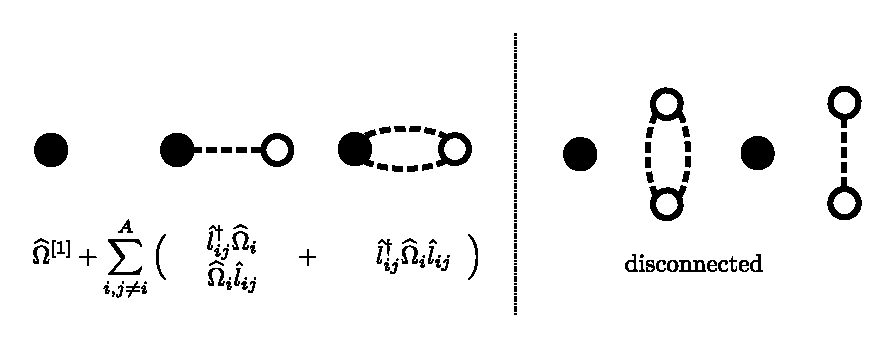
\includegraphics[scale=0.75]{figures/one_body_with_eq.pdf}
\caption{
The diagrammatic representation of the LCA expansion of a one-body operator (Eq.~(\ref{eq:LCA_one_body})).
Below each diagram is their corresponding expression.
The black dot represents the particle ``$i$'' on which the operator $\widehat{\Omega}_{i}$ is acting on.
The dashed lines are the correlation operator $\hat{l}_{ij}$ acting the particle pair ``$ij$''.
In the LCA, two dashed lines (correlation operators) are required to connect the same pair.
Disconnected diagrams are not considered in the LCA.
} 
\label{fig:LCA_one_body_diagram}
\end{figure}
%
\begin{figure}
\centering
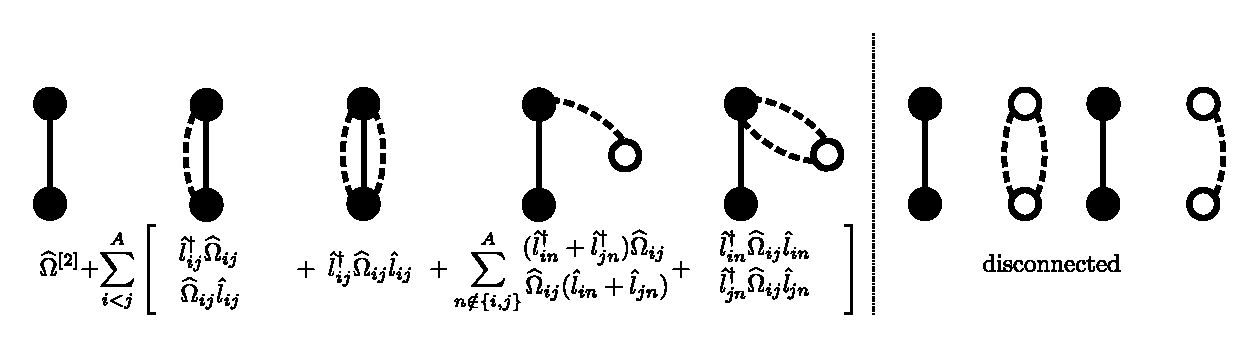
\includegraphics[scale=0.75]{figures/two_body_with_eq.pdf}
\caption{
The diagrammatic representation of the LCA expansion of a two-body operator (Eq.~(\ref{eq:LCA_one_body})).
Below each diagram is their corresponding expression.
The black dots represent the particle pair ``$ij$'' on which the operator $\widehat{\Omega}_{ij}$ is acting on.
The dashed lines are the correlation operator $\hat{l}_{in}$ acting the particle pair ``$in$''.
In the LCA, two dashed lines (correlation operators) are required to connect the same pair.
Disconnected diagram are not considered in the LCA.
} 
\label{fig:LCA_two_body_diagram}
\end{figure}
\section{Momentum distributions}
\subsection{Second quantization}
This section will be somewhat over-elaborated. But it can serve as a recapitulation of second quantization.

The one body momentum distribution operator is defined as,
\begin{align}
	\hat{n}(p) = \frac{1}{(2 \pi)^{3}} \int \textrm{d}^{2} \Omega_{\mathbf{p}} a_{\mathbf{p}}^{\dagger} a_{\mathbf{p}}
\end{align}
It's action on a multi particle ground state $\ket{\Phi}$,
\begin{align}
	\braket{ \Phi | \hat{n}(p) | \Phi} = \frac{1}{(2 \pi)^{3}} \int \textrm{d}^{2} \Omega_{\mathbf{p}} \braket{ \Phi | a_{\mathbf{p}}^{\dagger} a_{\mathbf{p}} | \Phi}
\end{align}
The creation and annihilation operators $a_{\mathbf{p}}^{\dagger}$,$a_{\mathbf{p}}$ have only meaning working on particles with definite momentum or the vacuum state $\ket{0}$.
\begin{align}
	\braket{ \Phi | a_{\mathbf{p}}^{\dagger} a_{\mathbf{p}} | \Phi} &= \int \textrm{d}^{3} \mathbf{p}_{1} \ldots \textrm{d}^{3} \mathbf{p}_{A} \braket {\Phi | \mathbf{p}_1 \mathbf{p}_2 \ldots \mathbf{p}_{A}} \braket{ \mathbf{p}_{1} \mathbf{p}_{2} \ldots \mathbf{p}_{A} | a_{\mathbf{p}}^{\dagger} a_{\mathbf{p}} | \Phi } \\
	&= \int \textrm{d}^{3} \mathbf{p}_{1} \ldots \textrm{d}^{3} \mathbf{p}_{A} \braket {\Phi | \mathbf{p}_1 \mathbf{p}_2 \ldots \mathbf{p}_{A}} \braket{ 0 | a_{\mathbf{p}_{1}} a_{\mathbf{p}_{2}} \ldots a_{\mathbf{p}_{A}} a_{\mathbf{p}}^{\dagger} a_{\mathbf{p}} | \Phi } 
\end{align}
Using the anticommutation relation $\{ a_{\mathbf{p}} ,a_{\mathbf{q}}^{\dagger} \} = \delta(\mathbf{p}-\mathbf{q})$, we get
\begin{align}
	\braket{0 | a_{\mathbf{p}_{1}} a_{\mathbf{p}_{2}} \ldots a_{\mathbf{p}_{A}} a_{\mathbf{p}}^{\dagger} a_{\mathbf{p}} | \Phi} &=
	\braket{0 | a_{\mathbf{p}_{1}} a_{\mathbf{p}_{2}} \ldots \delta(\mathbf{p}-\mathbf{p}_{A}) a_{\mathbf{p}} | \Phi} - \braket{0 | a_{\mathbf{p}_{1}} a_{\mathbf{p}_{2}} \ldots a_{\mathbf{p}_{A-1}} a_{\mathbf{p}}^{\dagger} a_{\mathbf{p}_{A}} a_{\mathbf{p}} | \Phi} \\
	&= \delta(\mathbf{p}-\mathbf{p}_{A}) \braket{\mathbf{p}_{1} \mathbf{p}_{2} \ldots \mathbf{p} | \Phi } - \delta(\mathbf{p}-\mathbf{p}_{A-1}) \braket{0 | a_{\mathbf{p}_1} \ldots a_{\mathbf{p}_{A-2}} a_{\mathbf{p}_{A}} a_{\mathbf{p}} | \Phi} \\
	&+ \braket{0| a_{\mathbf{p}_1} \ldots a_{\mathbf{p}_{A-2}} a_{\mathbf{p}}^{\dagger} a_{\mathbf{p}_{A-1}} a_{\mathbf{p}_{A}} a_{\mathbf{p}} | \Phi} \\
 &= \delta(\mathbf{p}-\mathbf{p}_{A}) \braket{\mathbf{p}_{1} \mathbf{p}_{2} \ldots \mathbf{p}_{A} | \Phi } + \delta(\mathbf{p}-\mathbf{p}_{A-1}) \braket{\mathbf{p}_{1} \ldots \mathbf{p}_{A-2} \mathbf{p}_{A-1} \mathbf{p}_{A} | \Phi} \\
	&+ \braket{0| a_{\mathbf{p}_1} \ldots a_{\mathbf{p}_{A-2}} a_{\mathbf{p}}^{\dagger} a_{\mathbf{p}_{A-1}} a_{\mathbf{p}_{A}} a_{\mathbf{p}} | \Phi}
	&= \ldots \\
	&= \sum_{i=1}^{A} \delta(\mathbf{p} - \mathbf{p}_{i}) \braket{ \mathbf{p}_{1} \ldots \mathbf{p}_{A} | \Phi} + (-1)^{A} \underbrace{\braket{ 0 | a_{\mathbf{p}}^{\dagger} a_{\mathbf{p}_1} \ldots a_{\mathbf{p}_{A}} a_{\mathbf{p}} | \Phi}}_{=0}
\end{align}
Hence,
\begin{align}
	\braket{ \Phi | a_{\mathbf{p}}^{\dagger} a_{\mathbf{p}} | \Phi} &= \int \textrm{d}^{3} \mathbf{p}_{1} \ldots \textrm{d}^{3} \mathbf{p}_{A} \braket {\Phi | \mathbf{p}_1 \mathbf{p}_2 \ldots \mathbf{p}_{A}} \sum_{i=1}^{A} \delta(\mathbf{p} - \mathbf{p}_{i}) \braket{ \mathbf{p}_{1} \mathbf{p}_{2} \ldots \mathbf{p}_{A} | \Phi}
\end{align}
If $\ket{\Phi}$ is a slater determinant of orthonormal single particle wave functions $\ket{\phi_{\alpha_{i}}}$ we get,
\begin{align}
	\braket{ \Phi | a_{\mathbf{p}}^{\dagger} a_{\mathbf{p}} | \Phi} &= \sum_{i=1}^{A} | \braket{ \mathbf{p} | \phi_{\alpha_{i}} } |^{2} = \sum_{i=1}^{A} \phi_{\alpha_i}^{\dagger}(\mathbf{p}) \phi_{\alpha_i}(\mathbf{p})
\end{align}
Note that we also could have derived this result by instead of inserting the unit $\prod_{i=1}^{A} \textrm{d}^{3} \mathbf{p}_{i} \ket{\mathbf{p}_{i}}\bra{\mathbf{p}_{i}}$ we expand $\ket{\Phi}$ in terms of single particle creation operators,
\begin{align}
	a_{\mathbf{p}}^{\dagger} a_{\mathbf{p}} \ket{\Phi} &= a_{\mathbf{p}}^{\dagger} a_{\mathbf{p}} \ket{ \alpha_1 \alpha_2 \ldots \alpha_A } = a_{\mathbf{p}}^{\dagger} a_{\mathbf{p}} a_{\alpha_1}^{\dagger} a_{\alpha_2}^{\dagger} \ldots a_{\alpha_A}^{\dagger} \ket{0}
\end{align}
The commutation relations between $a_{\mathbf{p}}$ and $a_{\alpha_i}$ are easily derived by expanding $a_{\alpha_i}$ in momentum creation operators,
\begin{align}
	a_{\alpha_i}^{\dagger} &= \int \textrm{d}^{3} \mathbf{k} \phi_{\alpha_i}(\mathbf{k}) a_{k}^{\dagger} \\
	\Rightarrow a_{\mathbf{p}} a_{\alpha_i}^{\dagger} &= \int \textrm{d}^{3} \mathbf{k} \phi_{\alpha_i}(\mathbf{k}) a_{\mathbf{p}} a_{\mathbf{k}}^{\dagger} = \phi_{\alpha_i}(\mathbf{p}) - a_{\alpha_i}^{\dagger} a_{\mathbf{p}}
\end{align}
So,
\begin{align}
	a_{\mathbf{p}} \ket{\Phi} &= a_{\mathbf{p}} a_{\alpha_1}^{\dagger} a_{\alpha_2}^{\dagger} \ldots a_{\alpha_A}^{\dagger} \ket{0} = (\phi_{\alpha_1}(\mathbf{p}) - a_{\alpha_1}^{\dagger} a_{\mathbf{p}}) a_{\alpha_2}^{\dagger} \ldots a_{\alpha_A}^{\dagger} \ket{0} \\
	&= \sum_{i=1}^{A} (-1)^{i-1} \phi_{\alpha_{i}}(\mathbf{p}) \ket{ \alpha_1 \ldots \alpha_{i-1} \alpha_{i+1} \ldots \alpha_A}
\end{align}
The conjugate gives,
\begin{align}
	\bra{\Phi} a_{\mathbf{p}}^{\dagger} &= \sum_{j=1}^{A} (-1)^{j-1} \bra{ \alpha_1 \ldots \alpha_{j-1} \alpha_{j+1} \ldots \alpha_A} \phi_{\alpha_j}^{\dagger}(\mathbf{p})
\end{align}
Hence,
\begin{align}
\braket{ \Phi | a_{\mathbf{p}}^{\dagger} a_{\mathbf{p}} | \Phi} &= \sum_{i,j=1}^{A} (-1)^{i+j} \phi_{\alpha_j}^{\dagger}(\mathbf{p}) \phi_{\alpha_{i}}(\mathbf{p})  \underbrace{\braket{ \alpha_1 \ldots \alpha_{j-1} \alpha_{j+1} \ldots \alpha_A | \alpha_1 \ldots \alpha_{i-1} \alpha_{i+1} \ldots \alpha_A }}_{=\delta_{ij}} \\
	&= \sum_{i} \phi_{\alpha_i}^{\dagger}(\mathbf{p}) \phi_{\alpha_{i}}(\mathbf{p})
\end{align}
Which is exactly the same result as before.



So the one body momentum distribution is given by,
\begin{align}
	\braket{ \Phi | \hat{n}(p) | \Phi} &=  \sum_{i=1}^{A} \frac{1}{(2 \pi)^{3}} \int \textrm{d}^{2} \Omega_{\mathbf{p}}\phi_{\alpha_i}^{\dagger}(\mathbf{p}) \phi_{\alpha_i}(\mathbf{p})
\end{align}
Note that this distribution is normed to the number of particles $A$. To get the momentum distribution normed to unity we have to divide by A,
\begin{align}
	\braket{ \Phi | \hat{n}(p) | \Phi} &=  \frac{1}{A} \sum_{i=1}^{A} \frac{1}{(2 \pi)^{3}} \int \textrm{d}^{2} \Omega_{\mathbf{p}}\phi_{\alpha_i}^{\dagger}(\mathbf{p}) \phi_{\alpha_i}(\mathbf{p})
\end{align}

\section{Nucleus}
\subsection{shell.h}
This class contains the quantum number of a shell $nlj$. It has two (proton \& neutron) static arrays containing all the shells.
\begin{verbatim}
	shellsN = [ Shell(n1,l1,j1), Shell(n2,l2,j2), ... ]
	shellsP = [ Shell(n1,l1,j1), Shell(n2,l2,j2), ... ]
\end{verbatim}
These two arrays are initialised and deleted by the static methods \texttt{Shell::initialiseShells}, \texttt{Shell::deleteShells}.

\subsection{nucleus.h}
First important method here is \texttt{Nucleus::makePairs}. Note that this relies on overloaded virtual functions to function. It iterates over the quantum numbers, $n_1 l_1 j_1 m_{j_1}, n_2 l_2 j_2 m_{j_2}$ and makes a pair for each of these combinations: \texttt{Pair::Pair(mosh,n1,l1,j1,mj1,t1,n2,l2,j2,mj2,t2)}. \texttt{mosh} is the return value of \texttt{RecMosh::createRecMosh(n1,l1,n2,l2,inputdir,outputdir)}, being a \texttt{RecMosh} object. The moshinsky brackets $\braket{n_1 l_1 n_2 l_2; \Lambda | n l N L ; \Lambda}$ can be accessed by calling \texttt{RecMosh::getCoefficient(n,l,N,L,Lambda)}.
Open shells are taken care of by calculating a open shell correction factor and applying it to the pair via \texttt{Pair::setfnorm(factor)}.

Once the pairs (\texttt{Pair::Pair}) are generated we can generate a 



\section{Pair coupling}
\subsection{pair.h}
This class represents the state
\begin{align}
	\ket{ \alpha_1, \alpha_2}_{\textrm{nas}} \;\;\;, \ket{\alpha} \equiv \ket{n l j m_j t m_t}
\end{align}
The class calculates all the coefficients,
\begin{align}
	C_{\alpha_1 \alpha_2}^{A} = \braket{A \equiv \{ n l S j m_j, N L M_L T M_T\} | \alpha_1 \alpha_2}_{\text{nas}}
	\label{eq:coef}
\end{align}
The main method here is \texttt{Pair::makecoeflist()}. It loops over all possible values of $ A \equiv \{ S,T,n,l,N,M_L,j,m_j \}$. Where in the summation over $\{n,l,N,L\}$ the energy conservation $2n_1 + l_1 + 2n_2 + l_2 = 2n + l + 2N + L$ is taken into account to eliminate one of the summation loops, $L = 2n_1 + l_1 + 2n_2 + l_2 - 2n - l - 2N$. Note that $M_T$ is also fixed by $M_T = m_{t_1} + m_{t_2}$ and no summation over this is performed, as we want to keep the contribution from different pairs separated.
For each $A$ a new object \texttt{Newcoef} is generated and stored in the member \texttt{std::vector<NewCoef*> coeflist}.
\subsection{newcoef.h}
This class takes the parameters $n_1 l_1 j_1 m_{j_1} m_{t_1} n_2 l_2 j_2 m_{j_2} m_{t_2} N L M_L n l S j m_j T M_T$, and calculates the coefficient given in Eq. (\ref{eq:coef}). It takes also a pointer to a \texttt{RecMosh} object that holds the Moshinsky brackets. The only function in this class is to calculate $C_{\alpha_1 \alpha_2}^{A}$ using the formula,
\begin{multline}
	\sum_{J M_J} \sum_{\Lambda} 
	\frac{1}{\sqrt{2}} [ 1 - (-1)^{l+S+T}] \braket{ t_1 m_{t_1} t_2 m_{t_2} | T M_T }
	\braket{ j_1 m_{j_1} j_2 m_{j_2} | J M_J}
	\braket{ j m_j L M_L | J M_J } \\
	\braket{ n l N L; \Lambda | n_1 l_1 n_2 l_2 ; \Lambda}_{\textrm{SMB}}
	\sqrt{2 \Lambda + 1} \sqrt{ 2j+1}
	\left\{
	\begin{array}{ccc}
		j & L & J \\
		\Lambda & S & l
	\end{array}
	\right\} \\
	\sqrt{2j_1 + 1} \sqrt{2j_2 + 1} \sqrt{ 2S + 1} \sqrt{ 2 \Lambda + 1}
	\left\{
	\begin{array}{ccc}
		l_1 & s_1 & j_1 \\
		l_2 & s_2 & j_2 \\
		\Lambda & S & J \\
	\end{array}
	\right\}
\end{multline}
It is easy to check that the result indeed depends on $\alpha_1, \alpha_2, A$. Note that it is always assumed that $s_i,t_i \equiv \frac{1}{2}$ as we are dealing with protons and neutrons.
This class also defines a \texttt{``key''} to be able to index the coefficients, \texttt{key = ``nlSjm\_j.NLM\_L.TM\_T''}.

\subsection{paircoef.h}
\label{ssec:paircoef}
This is a very thin class designed to do some bookkeeping. As outlined in Maartens thesis pg 156, different $\ket{\alpha_1 \alpha_2}$ combinations will sometimes map to the same ``rcm'' states $A = \ket{ nlSjm_j NLM_L TM_T}$. In matrix element calculations,
\begin{align}
	\braket{\alpha_1 \alpha_2 | \hat{\mathcal{O}} | \alpha_1 \alpha_2} = \sum_{AB} C_{\alpha_1 \alpha_2}^{A \dagger} C_{\alpha_1 \alpha_2}^{B} \braket {A | \hat{\mathcal{O}} | B }
	\label{eq:rcm_nonzerodiag}
\end{align}
We want to calculate matrix elements as $\braket{ A | \hat{\mathcal{O}} | B}$ only once. $\ket{\alpha_1 \alpha_2}$ that map to the same $A,B$ states should lookup the earlier calculated values for $\braket{ A | \hat{\mathcal{O}} | B}$.
In general the matrix element $\braket{ A | \hat{\mathcal{O}} | B }$ is not diagonal. 
A \texttt{Paircoef} object has all the quantum numbers in a rcm state $A$. In addition it holds a value and a map \texttt{ std::map<Paircoef*, double>}. The map is used to link a rcm state $\ket{A}$ to all other rcm states $\ket{B}$ which yield a non zero contribution for $\braket{ A | \hat{\mathcal{O}} | B }$. The value for the transformation coefficients $C_{\alpha_1,\alpha_2}^{A,\dagger} C_{\alpha_1,\alpha_2}^{B}$ is stored in the second field of the map (\texttt{double}). So that the the summation over $B$ (Eq. \ref{eq:rcm_nonzerodiag}) is replaced by,
\begin{align}
	\braket{\alpha_1 \alpha_2 | \hat{\mathcal{O}} | \alpha_1 \alpha_2} = \sum_{A} \sum_{\texttt{Paircoef(A).links}}  \texttt{link.strength} \braket {A | \hat{\mathcal{O}} | B }
\end{align}
\todo[inline]{\texttt{Paircoef::add(double val)} adds \texttt{val} to private member \texttt{value} but as far as I can see this private member \texttt{value} is NEVER used!}
Note that the ``linked'' rcm states $\ket{A},\ket{B}$ both stem from the expansion of the same single particle state $\ket{ \alpha_1 \alpha_2}$.
This means that the linked rcm states will have certain properties.
For example, the parity of $\ket{ \alpha_1 \alpha_2}$ is given by $(-1)^{l_1 + l_2}$, the parity of a rcm state is $(-1)^{l+L}$, with $l$ the relative angular momentum and $L$ the c.m. angular momentum.
Conservation of parity means that $(-1)^{l_1 + l_2} = (-1)^{l_A + L_A} = (-1)^{l_B + L_B}$.
For example, for operators that do not change the total spin $S$ (this is the case for the operators considered here), we have $S_A = S_B$, it then follows that
\begin{itemize}
	\item if $T_A=T_B$ then $l_A$ and $l_B$ have the same even-odd parity because of $l+S+T=$ odd.
	From $l_A - l_B$ is even it then follows that $L_A - L_B$ is even, or $L_A,L_B$ have the same even-odd parity.
	\item if $T_A \neq T_B$ then $l_A$ and $l_B$ have opposite even-odd parity. Resulting in the condition that $L_A$ and $L_B$ also must have different even-odd parity. 
\end{itemize}

\section{Matrix Elements}
First some theory on the matrix elements. In the calculation of the norm we only have the correlation operator $\hat{\wr}$ between the bras and kets.
\begin{align}\label{eq:norm}
	\braket{ \alpha \beta |\hat{\wr}(\vec{x}_{1},\vec{x}_{2}) + \hat{\wr}^{\dagger}(\vec{x}_{1},\vec{x}_{2}) + \hat{\wr}^{\dagger}(\vec{x}_{1},\vec{x}_{2})\hat{\wr}(\vec{x}_{1},\vec{x}_{2}) | \alpha \beta}
\end{align}
$\hat{\wr}$ contains a central, tensor and spin-isospin part,
\begin{align*}
	\hat{\wr}(\vec{x}_{1},\vec{x}_{2}) = -f_c(r_{12}) + f_{t\tau}(r_{12}) \hat{S}_{12} \hat{\vec{\tau}}_{1} \cdot \hat{\vec{\tau}}_{2} + f_{\sigma \tau}(r_{12}) \hat{ \vec{\sigma}}_{1} \cdot \hat{ \vec{\sigma}}_{2} \hat{ \vec{\tau}}_{1} \cdot \hat{ \vec{\tau}}_{2}  \, .
\end{align*}
Transforming to the c.m. and relative coordinates a general matrix-element term can be written as,
\begin{align*}
	\braket{ n (l S) j m_j N L M_L T M_T |  \hat{\mathcal{O}}^{p\dagger} f^{\dagger}_{p} f_{q} \hat{\mathcal{O}}^{q} | n' (l' S') j' m_j' N' L' M_L' T' M_T'} 
\end{align*}
With $f_{p,q} \in \{ 1, f_{c}, f_{t\tau}, f_{\sigma \tau} \}$ and $\hat{\mathcal{O}}^{p,q}$ the corresponding operator $\in \{ \mathbb{1}, \mathbb{1},  \hat{S}_{12} \hat{\vec{\tau}}_{1} \cdot \hat{\vec{\tau}}_{2}, \hat{ \vec{\sigma}}_{1} \cdot \hat{ \vec{\sigma}}_{2} \hat{ \vec{\tau}}_{1} \cdot \hat{ \vec{\tau}}_{2} \} $.
As no operators act on the c.m. part $ \ket{ N L M_L}$ here we have,
\begin{align*}
	\delta_{NN'} \delta_{LL'} \delta_{M_L M_L'} \braket{ n (l S) j m_j T M_T |  \hat{\mathcal{O}}^{p\dagger} f^{\dagger}_{p} f_{q} \hat{\mathcal{O}}^{q} | n' (l' S') j' m_j' T' M_T'}  
\end{align*}
Let us now take a look at the separate cases for $\delta_{NN'} \delta_{LL'} \delta_{M_L M_L'} \braket{ n (l S) j m_j T M_T |  \hat{\mathcal{O}}^{p\dagger} f^{\dagger}_{p} f_{q} \hat{\mathcal{O}}^{q} | n' (l' S') j' m_j' T' M_T'} $,
\begin{itemize}
	\item $\hat{\mathcal{O}}^{p} = \mathbb{1}$, $f_{p} = 1$, $\hat{\mathcal{O}}^{q} = \mathbb{1}$ , $f_{q} = f_c(r_{12})$ 
	\begin{multline*}
		\delta_{NN'} \delta_{LL'} \delta_{M_L M_L'} \braket{ n (l S) j m_j T M_T |  f_{c}(r_{12}) | n' (l' S') j' m_j' T' M_T'}  \\
		= \delta_{NN'} \delta_{LL'} \delta_{M_L M_L'} \delta_{SS'} \delta_{jj'} \delta_{m_j m_j'} \delta_{TT'} \delta_{M_T M_T'} \delta_{l l'} \braket{ n l |  f_{c}(r_{12}) | n' l'} 
	\end{multline*}
	\begin{multline*}
		\braket{ n l |  f_{c}(r_{12}) | n' l'} = \int \text{d} r_{12} \, r_{12}^{2} R_{nl}(r_{12}) f_{c}(r_{12}) R_{n'l'}(r_{12}) \\
	\end{multline*}
	With  $R_{nl}(r) = \left[ \frac{2n!}{\Gamma(n + l + 3/2)} \nu^{l + 3/2} \right]^{\frac{1}{2}} r^{l} e^{-\nu r^{2} /2} L_{n}^{l+1/2}(\nu r^{2}) = N_{nl} \nu^{\frac{l + 3/2}{2}} r^{l} e^{-\nu r^{2} /2} L_{n}^{l+1/2}(\nu r^{2})$ and $ \nu = M_N \omega / \hbar $.
	\begin{multline*}
		\braket{ n l |  f_{c}(r_{12}) | n' l'} = N_{nl} N_{n'l'} \nu^{\frac{l + l' + 3}{2}} \int \text{d} r_{12} \, r_{12}^{2} r_{12}^{l} e^{-\nu r_{12}^{2} /2} L_{n}^{l+1/2}(\nu r_{12}^{2}) f_{c}(r_{12}) r_{12}^{l'} e^{-\nu r_{12}^{2} /2} L_{n'}^{l'+1/2}(\nu r_{12}^{2}) \\
	\end{multline*}
	The correlation functions $f_{p}(r)$ are expanded as $ \sum_{\lambda}^{\lambda_{\text{max}}} b_{\lambda} r^{\lambda} e^{-b r^{2}}$.
	In the current parameterization of the correlation functions it appears that $\lambda_{\text{max}} = 10$ for the central correlation function and $\lambda_{\text{max}}=9$ for the tensor and spin-isospin correlation functions.
	Expanding the generalized laguerre polynomials as $ L_{n}^{l}(r) = \sum_{k} a_{nl,k} r^{k}$ results in,
	\begin{multline*}
		\braket{ n l |  f_{c}(r_{12}) | n' l'} = N_{nl} N_{n'l'} \nu^{\frac{l + l' + 3}{2}} \sum_{kk'\lambda} a_{nl,k} a_{n'l',k'} b_{\lambda}  \int \text{d} r_{12} r_{12}^{2+l+l'} e^{-\nu r_{12}^{2}} ( \nu r_{12}^{2} )^{k} r_{12}^{\lambda} e^{-b r_{12}^{2}} ( \nu r_{12}^{2})^{k'}
	\end{multline*}
	With the substitution $r = \sqrt{\nu} \, r_{12}, B = b/\nu$ (units are $[\nu] = \text{m}^{-2}, [b] = \text{m}^{-2}, [r] = 1, [B] = 1$) we get,
	\todo[inline]{Maarten says $B = b/\sqrt{\nu}$ (D.19), I think this is incorrect (units do not match), $Bx^{2}$ of (D.19) is NOT dimensionless while it should be... (appears to be correct in the code however...)}
	\begin{multline}
		\braket{ n l |  f_{c}(r_{12}) | n' l'} = N_{nl} N_{n'l'} \nu^{\frac{l + l' + 3}{2}} \sum_{kk'\lambda} a_{nl,k} a_{n'l',k'} b_{\lambda}  \nu^{- \frac{3 + l + l' + \lambda}{2}} \int \text{d} r \, r^{2+l+l'} e^{-r^{2}} r^{2k} r^{\lambda} e^{-B r^{2}} r^{2k'} \\
		= N_{nl} N_{n'l'} \sum_{kk'\lambda} \nu^{-\frac{\lambda}{2}}  a_{nl,k} a_{n'l',k'} b_{\lambda} \int \text{d} r \, r^{2+l+l'+\lambda + 2k + 2k'} e^{-(B+1) r^{2}} \\
		=  N_{nl} N_{n'l'}  \sum_{kk'\lambda} \nu^{-\frac{\lambda}{2}} a_{nl,k} a_{n'l',k'} b_{\lambda} \frac{1}{2} \Gamma \left( \frac{K+1}{2} \right) (1 + B)^{-\frac{K+1}{2}} \\
		= \frac{N_{nl} N_{n'l'}}{2}  \sum_{kk'\lambda} \nu^{-\frac{\lambda}{2}} a_{nl,k} a_{n'l',k'} b_{\lambda} \Gamma \left( \frac{K+1}{2} \right) (1 + B)^{-\frac{K+1}{2}}
		\label{eq:central_corr_single}
	\end{multline}
	$K = 2+l+l'+ \lambda + 2k + 2k'$. To recapitulate, $a_{nl,k}$ is the $k$'th expansion coefficient of the Laguerre polynomials. The sum over $k$ ($k'$) ranges from $0$ to $n$ ($n'$). $b_{\lambda}$ is the $\lambda$'th expansion coefficient of the correlation function, runs from $0$ to a finite value ($10$ or $11$ for Maartens' fits). $\nu = M_N \omega /\hbar$ is the H.O.-potential parameter and is nucleus dependent. $N_{nl} = \left[ \frac{2n!}{\Gamma(n + l + 3/2)} \right]^{\frac{1}{2}} = \left[ \frac{ 2 \, \Gamma( n + 1)}{\Gamma(n + l + 3/2)} \right]^{\frac{1}{2}} $ are the normalisation factors of the orbital wave functions, these factors are nucleus independent (only $n,l$ dependencies).

	Orthonormality using this expansion (Eq.~\ref{eq:central_corr_single}) can easily be checked, $\braket{ n l |  1 | n' l}$ ($l=l'$ because of the orthonormality of the spherical harmonics), if we set $b_{\lambda} = \delta_{\lambda,0}$, $b=0$.
	\begin{align}
		\braket{ n l |  1 | n' l} =  \frac{N_{nl} N_{n'l}}{2}  \sum_{kk'=0}^{nn'} a_{nl,k} a_{n'l,k'} \Gamma \left( \frac{3+2l+2k + 2k'}{2} \right)
	\end{align}
	\item $\hat{\mathcal{O}}^{p} = \mathbb{1}$, $f_{p} = f_c(r_{12})$, $\hat{\mathcal{O}}^{q} = \mathbb{1}$ , $f_{q} = f_c(r_{12})$, the non trivial part of the matrix element now comes down to calculating,
	\begin{multline*}
		\braket{ n l |  f_{c}^{2}(r_{12}) | n' l'} = \int \text{d} r_{12} \, r_{12}^{2} R_{nl}(r_{12}) f_{c}^{2}(r_{12}) R_{n'l'}(r_{12}) \\
		= N_{nl} N_{n'l'} \nu^{\frac{l + l' + 3}{2}} \sum_{kk'\lambda \lambda'} a_{nl,k} a_{n'l',k'} b_{\lambda} b_{\lambda'}  \int \text{d} r_{12} r_{12}^{2+l+l'} e^{-\nu r_{12}^{2}} ( \nu r_{12}^{2} )^{k} r_{12}^{\lambda+\lambda'} e^{-2 b r_{12}^{2}} ( \nu r_{12}^{2})^{k'} \\
		= N_{nl} N_{n'l'} \nu^{\frac{l + l' + 3}{2}} \sum_{kk'\lambda \lambda'} a_{nl,k} a_{n'l',k'} b_{\lambda} b_{\lambda'} \nu^{- \frac{3 + l + l' + \lambda + \lambda'}{2}} \int \text{d} r \, r^{2+l+l'+2k+2k'+\lambda + \lambda'} e^{- ( 2B + 1) r^{2}} \\
		=  \frac{N_{nl} N_{n'l'}}{2} \sum_{kk'\lambda \lambda'} \nu^{ - \frac{\lambda + \lambda'}{2}} a_{nl,k} a_{n'l',k'} b_{\lambda} b_{\lambda'} \Gamma\left(\frac{K+1}{2}\right) (2B+1)^{-\frac{K+1}{2}}
	\end{multline*}
	With $K = 2+l+l'+2k+2k'+\lambda+\lambda'$ and $B = b/\nu$
\end{itemize}
\section{Matrix elements bis}

Let us take a look at
\begin{align*}
	\braket{ S | \hat{ \vec{\sigma}}_{1} \cdot \hat{ \vec{\sigma}}_{2} | S'} = 2 \braket{ S | \hat{ \vec{s}}_{1} \cdot \hat{ \vec{s}}_{2} | S'} = 4 \braket{ S | \hat{\vec{S}}^{\, 2} - \hat{\vec{s}}_{1}^{\,2} - \hat{\vec{s}}_{2}^{\,2} | S'} = 2 ( S(S+1) - \frac{3}{4} - \frac{3}{4} ) \delta_{SS'} = \delta_{SS'} (2 S(S+1) - 3)
\end{align*}
As we have 2 spin $1/2$ particles S can be either $0,1$ resulting in $\braket{ 1 | \hat{ \vec{\sigma}}_{1} \cdot \hat{ \vec{\sigma}}_{2} | 1} = 1$, $\braket{ 0 | \hat{ \vec{\sigma}}_{1} \cdot \hat{ \vec{\sigma}}_{2} | 0} = -3$.
\todo[inline]{ Note that in the Maartens code the expression is modified to $4S-3$, which is equivalent for $S \in \{0,1\} $.} As this is independent of the spin projection $M_S$ we have,
\begin{align*}
	\braket{ S M_S | \hat{ \vec{\sigma}}_{1} \cdot \hat{ \vec{\sigma}}_{2} | S' M_S'} = \delta_{SS'} \delta_{M_S M_S'} (2 S(S+1) - 3)
\end{align*}
Exactly the same derivation can be made for $\hat{\vec{\tau}}_{1} \cdot \hat{\vec{\tau}}_{2}$ leading to the same result.
\begin{align*}
	\braket{ T M_T | \hat{\vec{\tau}}_{1} \cdot \hat{\vec{\tau}}_{2} | T' M_T'} = \delta_{TT'} \delta_{M_T M_T'} (2 T(T+1) - 3)
\end{align*}
When selecting a a specific isospin projection $m_t = \pm 1/2 $ (proton or neutron) of a nucleon this result changes however.
The product $\hat{\vec{\tau}}_{1} \cdot \hat{\vec{\tau}}_{2}$ written in the spherical basis becomes,
\begin{align*}
	\hat{\vec{\tau}}_{1} \cdot \hat{\vec{\tau}}_{2} = \hat{\tau}_{1,0} \hat{\tau}_{2,0} - \hat{\tau}_{1,+} \hat{\tau}_{2,-} - \hat{\tau}_{1,-} \hat{\tau}_{2,+} = \hat{\tau}_{1,0} \hat{\tau}_{2,0} + \frac{\hat{\tau}_{1}^{+} \hat{\tau}_{2}^{-}}{2} + \frac{ \hat{\tau}_{1}^{-} \hat{\tau}_{2}^{+}}{2}
\end{align*}
Where $\hat{\tau}^{\pm}$ are the raising/lowering operators. Transitioning to the operators $\hat{t} = \hat{\tau}/2$ (analogues to the spin case $\hat{S} = \hat{\sigma}/2$) with the properties,
\begin{align*}
\hat{t}_0 \ket{ t, m_t} &= m_t \ket{ t, m_t} \\
\hat{t}^{\pm} \ket{ t, m_t} &= \sqrt{ t(t+1) - m(m \pm 1)} \ket { t, m_t \pm 1}.
\end{align*}
we get
\begin{align*}
	\hat{\vec{\tau}}_{1} \cdot \hat{\vec{\tau}}_{2} = 4 \hat{t}_{1,0} \hat{t}_{2,0} + 2 \hat{t}_{1}^{+} \hat{t}_{2}^{-} + 2 \hat{t}_{1}^{-} \hat{t}_{2}^{+} 
\end{align*}

Defining the isospin-projection operator acting on particle ``$i$'' of the 
nucleon pair $ \hat{\delta}_{m_t}^{[i]} = ( 1 + (2 m_t) \hat{t}_{i,0})/2$ we 
get,
\begin{multicols}{2}
\noindent
\begin{align*}
	\hat{\delta}_{m_t}^{[1]} \ket{ 1, \pm 1} &= \delta_{\pm 1,2m_t}  \ket{ 1, \pm 1}  \\
	\hat{\delta}_{m_t}^{[1]} \ket{ 1,0} &= \frac{1}{\sqrt{2}} \ket{ \frac{1}{2}, m_t} \otimes \ket{ \frac{1}{2}, -m_t} \\
	\hat{\delta}_{m_t}^{[1]} \ket{ 0,0} &= \frac{1}{\sqrt{2}} 2 m_t \ket{ \frac{1}{2}, m_t} \otimes \ket{ \frac{1}{2}, -m_t}
\end{align*}
\begin{align*}
	\hat{\delta}_{m_t}^{[2]} \ket{ 1, \pm 1} &= \delta_{\pm 1,2m_t}  \ket{ 1, \pm 1}  \\
	\hat{\delta}_{m_t}^{[2]} \ket{ 1,0} &= \frac{1}{\sqrt{2}} \ket{ \frac{1}{2}, -m_t} \otimes \ket{ \frac{1}{2}, m_t} \\
	\hat{\delta}_{m_t}^{[2]} \ket{ 0,0} &= \frac{1}{\sqrt{2}} (-2 m_t) \ket{ \frac{1}{2}, m_t} \otimes \ket{ \frac{1}{2}, -m_t}
\end{align*}
\end{multicols}
Note that sgn$(m_t) \equiv 2m_t$ as $m_t = \pm 1/2$.
It is straightforward to show that,
\begin{multicols}{2}
\noindent
\begin{align*}
	\braket{ 1, \pm 1 | \hat{\delta}_{m_t}^{[1]} | 1, \pm 1} &= \delta_{\pm 1,2m_t}  \\
	\braket{ 1,0 | \hat{\delta}_{m_t}^{[1]} | 1,0} = \braket{ 0,0 | \hat{\delta}_{m_t}^{[1]} | 0,0} &=  \frac{1}{2} \\
	\braket{ 1,0 | \hat{\delta}_{m_t}^{[1]} | 0,0} = \braket{ 0,0 | \hat{\delta}_{m_t}^{[1]} | 1,0} &=  \frac{1}{2} 2 m_t
\end{align*}
\begin{align*}
	\braket{ 1, \pm 1 | \hat{\delta}_{m_t}^{[2]} | 1, \pm 1} &= \delta_{\pm 1,2m_t}  \\
	\braket{ 1,0 | \hat{\delta}_{m_t}^{[2]} | 1,0} = \braket{ 0,0 | \hat{\delta}_{m_t}^{[1]} | 0,0} &=  \frac{1}{2} \\
	\braket{ 1,0 | \hat{\delta}_{m_t}^{[2]} | 0,0} = \braket{ 0,0 | \hat{\delta}_{m_t}^{[1]} | 1,0} &=  \frac{1}{2} (-2 m_t) 
\end{align*}
\end{multicols}

\subsection{norm\_ob : public operator\_virtual\_ob}
Here we take a look at the calculation of the norm $\mathcal{N}$ (see 
Eqs.~(\ref{eq:LCA_norm_one_body}),(\ref{eq:LCA_norm_two_body})) in 
\texttt{norm\_ob.cpp}.
Note that this class inherits from \texttt{operator\_virtual\_ob}, declaring general one body member functions.
\begin{itemize}
	\item \texttt{norm\_ob::get\_me( Pair )}.
		This calculates the matrix element \textbf{meanfield} matrix element sum:
		\begin{equation}
		\frac{2}{A} \sum_{ A B } \hat{\delta}_{t_1,n_A,l_A,n_B,l_B} C_{\alpha_1 \alpha_2}^{A \dagger} C_{\alpha_1 \alpha_2}^{B} \braket{ A|B} = \frac{2}{A} \sum_{A} \hat{\delta}_{t_1,n_A,l_A} \left| C_{\alpha_1 \alpha_2}^{A} \right|^{2}
		\end{equation}
		for a specific pair $\ket{\alpha_1 \alpha_2}$ passed trough \texttt{Pair}.
		It is possible to filter on relative quantum numbers on $n_A,l_A,n_B,l_B$, represented by the operator $\hat{\delta}_{t_1,n_A,l_A,n_B,l_B}$. It selects specific contributions \texttt{nAs,lAs,nBs,lBs} to the sum. A value of $-1$ for these variables is interpreted as ``all values allowed''. Trough the bracket $\braket{ A | B }$ we already have $n_A = n_B := n$, $l_A = l_B := l$.
		\begin{itemize}
			\item \texttt{if (nAs > -1 \&\& nBs > -1)}
				This forces $\texttt{nAs} = \texttt{nBs} = n$. So for $\texttt{nAs} \neq \texttt{nBs}$ we will get $0$.
			\item \texttt{if (nAs == -1 \&\& nBs > -1)}
				This forces $\texttt{nBs} = n$. Selecting a specific $n = n_A = n_B$ contribution.
			\item \texttt{if (nAs > -1 \&\& nBs == -1)}
				This forces $\texttt{nAs} = n$. Selecting a specific $n = n_A = n_B$ contribution.
			\item \texttt{if (nAs == -1 \&\& nBs == -1)}
				This makes no restrictions on $n = n_A = n_B$.
		\end{itemize}
		The exact same is valid for $l = l_A = l_B$ and \texttt{lAs},\texttt{lBs}.
		A few examples (\texttt{nAs,lAs,nBs,lBs}):
		\begin{itemize}
			\item (\texttt{-1, 2,-1,-1}) : allow all $n = n_A = n_B$ values. Restriction on $l = l_A = l_B = \texttt{2}$.
			\item (\texttt{-1, 2,-1, 2}) : allow all $n = n_A = n_B$ values. Restriction on $l = l_A = l_B = \texttt{2}$.
		\end{itemize}
	As the unrestricted sum $\sum_{ A B } C_{\alpha_1 \alpha_2}^{A \dagger} C_{\alpha_1 \alpha_2}^{B} \braket {A | B } = \sum_{A} | C^{A}_{\alpha_1 \alpha_2}|^{2} $ equals 1, the return value of \texttt{get\_me} (for the unrestricted sum) is,
	\begin{itemize}
		\item $\frac{2}{A}$ with no restriction on the isospin ( \texttt{norm\_ob::norm\_ob\_params.t = 0})
		\item $\frac{2}{A}$ for pp-pairs, $\frac{1}{A}$ for pn-pairs and $0$ for nn-pairs for a proton (\texttt{norm\_ob::norm\_ob\_params.t~=~1})
		\item $0$ for pp-pairs, $\frac{1}{A}$ for pn-pairs and $\frac{2}{A}$ for nn-pairs for a neutron (\texttt{norm\_ob::norm\_ob\_params.t~=-1})
	\end{itemize}
	If we sum over all the pairs $ \sum_{\texttt{pair in pairs}} $ \texttt{norm::ob\_get\_me(pair,...)} we get,
	\begin{itemize}
		\item $\frac{A(A-1)}{2} \frac{2}{A} = A-1$ with no restriction on the isospin ( \texttt{norm\_ob::norm\_ob\_params.t~=~0})
		\item $\frac{Z(Z-1)}{2}\frac{2}{A} + NZ \frac{1}{A} + \frac{N(N-1)}{2} 0 = Z \frac{A-1}{A}$ for a proton (\texttt{norm\_ob::norm\_ob\_params.t~=~1})
		\item $\frac{Z(Z-1)}{2}0 + NZ \frac{1}{A} + \frac{N(N-1)}{2} \frac{2}{A} = N \frac{A-1}{A}$ for a neutron (\texttt{norm\_ob::norm\_ob\_params.t~=-1})
	\end{itemize}
	\todo[inline,caption={}]{
	\textbf{Open shellness not taken into account here. Must be done somewhere else (higher up)...} \\	
	For closed shell nuclei everything seems fine. For open shells however we get some strange results. For example $^{27}$Al with $13$ protons and $14$ neutrons has an open $1d\frac{5}{2}$ proton shell. Open-shell nuclei are treated as closed shell but the pairs in the open shells get a weight factor. This weight factor however is \textbf{not} present in the method \texttt{norm::ob\_get\_me(pair,...)}. Hence as $A = 27$ but the closed shell equivalent with $A=28$ causes the number of pairs to be $28\cdot 27 /2$ instead of $ 27 \cdot 26 /2$. We get
	\begin{itemize}
	\item $ \frac{ 28 \cdot 27}{2} \frac{2}{27} = 28$ ( \texttt{norm\_ob::norm\_ob\_params.t = 0}) 
	\item $ \frac{ 14 \cdot 13}{2} \frac{2}{27} + \frac{14 \cdot 14 }{27} = \frac{378}{27} = 14 $ (\texttt{norm\_ob::norm\_ob\_params.t~=~1}) \\
	\item $ \frac{14 \cdot 14 }{27} + \frac{ 14 \cdot 13}{2} \frac{2}{27} = \frac{378}{27} = 14 $ (\texttt{norm\_ob::norm\_ob\_params.t~=-~1}) \\
	\end{itemize}
	}
	\item \texttt{norm\_ob::get\_me\_corr\_right( Pair )}.
\end{itemize}

\subsection{ density\_ob\_integrand3 }
Here we look at the file \texttt{density\_ob\_integrand3}. See section \ref{ssec:cm_mom_integral} for more information. The following integral is calculated,
\begin{align*}
\int \text{d} P_{12} \, P_{12}^{2} \Pi^{*}_{N L}(P_{12}) \Pi_{N' L'}(P_{12}) \chi_{p,nl_p}^{l_1 k}(p_1,P_{12}) \chi_{p,n'l_q'}^{l_1 k'}(p_1,P_{12}) 
\end{align*}
The symbols $\chi_{p,nl_p}^{l_1 k}(p_1,P_{12})$, $\chi_{p,n'l_q'}^{l_1 
k'}(p_1,P_{12})$ are calculated in \texttt{density\_ob\_integrand\_cf}. Hence 
this integrand takes two \texttt{density\_ob\_integrand\_cf*} pointers. 
Additionally it takes the parameters, 
$n,l_p,k,n',l_q',k',p_1,\nu,\texttt{index}$ 
(\texttt{nA,lA,la,nB,lB,l,k,nu,index} in the code). \texttt{index} corresponds 
to the power of $P_{12}$ in the integrand. This is because the $\Pi^{*}_{N 
L}(P_{12}) \Pi_{N' L'}(P_{12})$ are expanded in powers of $P_{12}$, again see 
\ref{ssec:cm_mom_integral} for more details.

\subsubsection{Alternative approach}
Here we will investigate an alternative approach of calculating the following integral,
\begin{align}
\int \text{d} P_{12} \, P_{12}^{2} \Pi^{*}_{N L}(P_{12}) \Pi_{N' L'}(P_{12}) \chi_{p,nl_p}^{kK}(p_1,P_{12}) \chi_{p,n'l_q'}^{k'K'}(p_1,P_{12}) 
\label{eq:alt_approach_start}
\end{align}
We will try to perform the integral over $P_{12}$ instead of keeping it last.
The $\chi$ symbols are defined as,
\begin{align*}
	\chi_{p,nl}^{kK}(p_1,P) = \int \text{d} r\, r^{2} f_{p}(r) R_{n l}(r) j_{k}( \sqrt{2} p_1 r)  j_{K}(P r)
\end{align*}
Eq.~(\ref{eq:alt_approach_start}) then becomes,
\begin{multline*}
\int \text{d} P_{12} \, P_{12}^{2} \Pi^{*}_{N L}(P_{12}) \Pi_{N' L'}(P_{12}) \chi_{p,nl_p}^{kK}(p_1,P_{12}) \chi_{p,n'l_q'}^{k'K'}(p_1,P_{12}) = \\
 \int \text{d} P_{12} \, P_{12}^{2} \Pi^{*}_{N L}(P_{12}) \Pi_{N' L'}(P_{12}) \\
 \int \text{d} r\, r^{2} f_{p}(r) R_{n l_p}(r) j_{k}( \sqrt{2} p_1 r)  j_{K}(P_{12} r) 
 \int \text{d} r' \, r^{\prime 2} f_{q}(r') R_{n l_q}(r') j_{k'}( \sqrt{2} p_1 r')  j_{K'}(P_{12} r') \, .
\end{multline*}
Expanding $\Pi_{NL}(P) = N_{NL} P^{L} e^{-\frac{\nu' P^{2}}{2}} \sum_{i=0}^{N} a_{NL,i} P^{i}$ and isolating the integral over $P_{12}$ results in,
\begin{multline*}
\int \text{d} P_{12} \, P_{12}^{2} \Pi^{*}_{N L}(P_{12}) \Pi_{N' L'}(P_{12}) \chi_{p,nl_p}^{kK}(p_1,P_{12}) \chi_{p,n'l_q'}^{k'K'}(p_1,P_{12}) = \\
 \int \text{d} r\, r^{2} f_{p}(r) R_{n l_p}(r) j_{k}( \sqrt{2} p_1 r)  
 \int \text{d} r' \, r^{\prime 2} f_{q}(r') R_{n l_q}(r') j_{k'}( \sqrt{2} p_1 r')   \\
  N_{NL} N_{N'L'} \sum_{i=0}^{N} \sum_{j=0}^{N'} a_{NL,i}  a_{N'L',j} 
 \int \text{d} P_{12} \, P_{12}^{2+L+L'+i+j} e^{-\nu' P_{12}^{2}} j_{K}(P_{12} r) j_{K'}(P_{12} r')
\end{multline*}
With $j_{l}(x) = \frac{\sqrt{\pi}}{2} \sum_{k=0}^{\infty} \frac{(-1)^{k}}{k! \Gamma(k+l+3/2)} \left( \frac{x}{2} \right)^{2k+l}$ this results in,
\begin{multline*}
\int \text{d} P_{12} \, P_{12}^{2} \Pi^{*}_{N L}(P_{12}) \Pi_{N' L'}(P_{12}) \chi_{p,nl_p}^{kK}(p_1,P_{12}) \chi_{p,n'l_q'}^{k'K'}(p_1,P_{12}) = \\
 \int \text{d} r\, r^{2} f_{p}(r) R_{n l_p}(r) j_{k}( \sqrt{2} p_1 r)  
 \int \text{d} r' \, r^{\prime 2} f_{q}(r') R_{n l_q}(r') j_{k'}( \sqrt{2} p_1 r')   \\
  N_{NL} N_{N'L'} \frac{ \pi}{4}  \sum_{i=0}^{N} \sum_{j=0}^{N'} a_{NL,i}  a_{N'L',j} 
 \sum_{s,s'} \frac{(-1)^{s+s'}}{s! s'! \Gamma(s+K+3/2) \Gamma(s'+K'+3/2)}  \left( \frac{r}{2} \right)^{2s+K} \left( \frac{r'}{2} \right)^{2s'+K'} \\
  \int \text{d} P_{12} \, P_{12}^{2+L+L'+i+j+2s+2s'+K+K'} e^{-\nu' P^{2}} \\
  = \int \text{d} r\, r^{2} f_{p}(r) R_{n l_p}(r) j_{k}( \sqrt{2} p_1 r)  
 \int \text{d} r' \, r^{\prime 2} f_{q}(r') R_{n l_q}(r') j_{k'}( \sqrt{2} p_1 r')   \\
  N_{NL} N_{N'L'} \frac{ \pi}{4}  \sum_{i=0}^{N} \sum_{j=0}^{N'} a_{NL,i}  a_{N'L',j} 
 \sum_{s,s'} \frac{(-1)^{s+s'}}{s! s'! \Gamma(s+K+3/2) \Gamma(s'+K'+3/2)}  \left( \frac{r}{2} \right)^{2s+K} \left( \frac{r'}{2} \right)^{2s'+K'} \\
  \frac{1}{2} \Gamma \left( \frac{3+L+L'+i+j+2s+2s'+K+K'}{2} \right) \nu^{\prime \, \frac{3+L+L'+i+j+2s+2s'+K+K'}{2} }
\end{multline*}
\subsection{ density\_ob\_integrand\_cf }
cf probably stands for correlation function. This class calculates integrals of the form
\begin{align*}
F_{p_1}(P) = \int dr r^{i+2} j_l(\frac{rP}{\sqrt{\nu}})  j_k(\frac{r p_1\sqrt{2}}{\sqrt{\nu}} )  f(\frac{r}{\sqrt{\nu}})  e^{\frac{-r^2}{2}}
\end{align*}
Where $p$ is the one-body momentum and $P$ is the c.m. momentum. This 
corresponds with the $\chi$ symbols defined below in Eq.~(\ref{eq:chi}).
\begin{align*}
	\chi_{p,nl}^{kK}(p_1,P) = \int \text{d} r\, r^{2} f_{p}(r) R_{n l}(r) j_{k}( \sqrt{2} p_1 r)  j_{K}(P r)
\end{align*}
With  $R_{nl}(r) = N_{nl} \nu^{\frac{l + 3/2}{2}} r^{l} e^{-\nu r^{2} /2} L_{n}^{l+1/2}(\nu r^{2})$ and $ \nu = M_N \omega / \hbar $,
\begin{align*}
	\chi_{p,nl}^{kK}(p_1,P) = N_{nl} \nu^{\frac{l + 3/2}{2}} \int \text{d} r\, r^{2+l} f_{p}(r)  e^{-\nu r^{2} /2} L_{n}^{l+1/2}(\nu r^{2}) j_{k}( \sqrt{2} p_1 r)  j_{K}(P r)
\end{align*}
Expanding the Generalized-Laguerre polynomials gives,
\begin{align*}
	\chi_{p,nl}^{kK}(p_1,P) = N_{nl} \nu^{\frac{l + 3/2}{2}} \sum_{i=0}^{n} a_{nl,i} \int \text{d} r\, r^{2+l} f_{p}(r)  e^{-\nu r^{2} /2}  (\nu r^{2})^{i} j_{k}( \sqrt{2} p_1 r)  j_{K}(P r)
\end{align*}
Changing variables $ r \rightarrow r/\sqrt{\nu}$ gives,
\begin{align*}
	\chi_{p,nl}^{kK}(p_1,P) =  N_{nl} \nu^{-\frac{3}{4}} \sum_{i=0}^{n} a_{nl,i} \int \text{d} r\, r^{2+l+2i} f_{p}( \nu^{-\frac{1}{2}} r)  e^{-r^{2} /2} j_{k}( \nu^{-\frac{1}{2}} \sqrt{2} p_1 r)  j_{K}(\nu^{-\frac{1}{2}} P r)
\end{align*}
This is exactly what is found in \texttt{density\_ob\_integrand\_cf::integrand} and \\ \texttt{density\_ob\_integrand\_cf::get\_value}.
The integrals are stored in a map where the key field contains the order of the spherical Bessel functions $k,K$ and is calculated as $100k+K$. It is necessary to assume that $ K < 100$.
The value field contains a two dimensional vector (\texttt{std::vector<std::vector<double>>}).
The first dimension (index) corresponds with the power of $r$ in the integrand and ranges from $0$ to $2n+l+2$.
The second dimension (index) corresponds with the different discretized values of $P$.
\section{One body operators acting on coupled states}
For a one body operator sandwiched between antisymmetric $A$-particle states $\ket{ \alpha_1 \alpha_2 \ldots \alpha_A}$ the following identity is valid,
\begin{align*}
	\sum_{i=1}^{A} \braket{ \alpha_1 \alpha_2 \ldots \alpha_A | \hat{\mathcal{O}}_{i} | \alpha_1 \alpha_2 \ldots \alpha_A} = A \braket{ \alpha_1 \alpha_2 \ldots \alpha_A | \hat{\mathcal{O}}_{1} | \alpha_1 \alpha_2 \ldots \alpha_A}
\end{align*}
In particular for two particles,
\begin{align*}
	\sum_{i=1}^{2} \braket{ \alpha_1 \alpha_2 | \hat{\mathcal{O}}_{i} | \alpha_1 \alpha_2} = 2 \braket{ \alpha_1 \alpha_2 | \hat{\mathcal{O}}_{1} | \alpha_1 \alpha_2}
\end{align*}
We now investigate how this result changes if we let the one-body operator act on coupled states of two particles. More specifically we will look at the one-body momentum operator $\hat{n}^{[1],i}_{s_1,t_1}(\vec{p}_1)$. The square brackets $[1]$ denote that this is a one-body operator. The number right next to that $i$ symbolizes which particle it acts on. $s,t$ denote the single-particle spin and isospin projections.
\begin{align*}
	\hat{n}^{[1],1}_{s_1,t_1}(\vec{p}_1) &= \hat{n}^{[1]}_{s_1,t_1}(\vec{p}_1) \otimes \mathbb{1} = \ket{\vec{p}_1 s_1 t_1} \bra{ \vec{p}_1 s_1 t_1} \otimes \sum_{s_2,t_2} \int \text{d}^{3} \, \vec{p}_{2} \ket{ \vec{p}_2 s_2 t_2} \bra{ \vec{p}_2 s_2 t_2} \\
	\hat{n}^{[1],2}_{s_1,t_1}(\vec{p}_1) &= \mathbb{1} \otimes \hat{n}^{[1]}_{s_1,t_1}(\vec{p}_1) = \sum_{s_2,t_2} \int \text{d}^{3} \, \vec{p}_{2} \ket{ \vec{p}_2 s_2 t_2} \bra{ \vec{p}_2 s_2 t_2} \otimes \ket{ \vec{p}_1 s_1 t_1} \bra{ \vec{p}_1 s_1 t_1} 
\end{align*}
We will try to relate $ \braket{ A | \hat{n}^{[1],2}_{s_1,t_1}(\vec{p}_1) | A'}$ to $ \braket{ A | \hat{n}^{[1],1}_{s_1,t_1}(\vec{p}_1) | A'}$. We will see that the naive expectation that these are equal does not hold. This is caused by the fact that we are sandwiching the one-body operator between \textbf{coupled} states and not single-particle states.
\begin{multline*}
	\braket{ A | \hat{n}^{[1],2}_{s_1,t_1}(\vec{p}_1)| A'} = \braket{ A | 
\mathbb{1} \otimes \hat{n}^{[1]}_{s_1,t_1}(\vec{p}_1) | A'} = \bra{ A } \left( 
\sum_{s_2,t_2} \int \text{d}^{3} \, \vec{p}_{2} \ket{ \vec{p}_2 s_2 t_2} \bra{ 
\vec{p}_2 s_2 t_2} \otimes \ket{ \vec{p}_1 s_1 t_1} \bra{ \vec{p}_1 s_1 t_1} 
\right) \ket{ A' } \\
	\propto \sum_{s_2,t_2} \int \text{d}^{3} \, \vec{p}_{2} \int \text{d}^{3} \, \vec{r}_{1} \text{d}^{3} \, \vec{r}_{1}^{\,\prime} \text{d}^{3} \vec{r}_{2} \text{d}^{3} \vec{r}_{2}^{\,\prime} \\
	\braket{ \widetilde{A} | \vec{r}_{1} \vec{r}_{2}} \braket { S M_S | \frac{1}{2} s_2 \frac{1}{2} s_1 } \braket{ T M_T | \frac{1}{2} t_2 \frac{1}{2} t_1 } \braket{ \vec{r}_{1} | \vec{p}_{2} } \braket{ \vec{r}_{2} | \vec{p}_{1}} \\
	\braket{ \vec{r}_{1}^{\,\prime} \vec{r}_{2}^{\,\prime} | \widetilde{A}'} \braket{ \frac{1}{2} s_2 \frac{1}{2} s_1 | S' M_S'} \braket{ \frac{1}{2} t_1 \frac{1}{2} t_2 | T' M_T'} \braket{ \vec{p}_2 | \vec{r}_{1}^{\,\prime}} \braket{ \vec{p}_{1} | \vec{r}_{2}^{\,\prime}} \\
\end{multline*}
Note that we used $\propto$ instead of the equality sign as we omit the LS-coupling for conciseness. This has no influence on the results. $\widetilde{A}$ symbolizes the coupled state without the spin and isospin part (with the LS-coupling omitted), $\widetilde{A} = \ket{ n l m_l N L M_L}$.  Using the identity,
\begin{align*}
	\braket{ j_1 m_1, j_2 m_2 | J M } &= (-1)^{j_1 + j_2 - J} \braket{ j_2 m_2, j_1 m_1 | J M} 
\end{align*}
we get
\begin{multline*}
	\braket{ A | \hat{n}^{[1],2}_{s_1,t_1}(\vec{p}_1)| A'}	\propto 
\sum_{s_2,t_2} \int \text{d}^{3} \, \vec{p}_{2} \int \text{d}^{3} \, \vec{r}_{1} 
\text{d}^{3} \, \vec{r}_{1}^{\,\prime} \text{d}^{3} \vec{r}_{2} \text{d}^{3} 
\vec{r}_{2}^{\,\prime} \\
	(-1)^{  S + S' + T + T'} \\
	\braket{ \widetilde{A} | \vec{r}_{1} \vec{r}_{2}} \braket { S M_S | \frac{1}{2} s_1 \frac{1}{2} s_2 } \braket{ T M_T | \frac{1}{2} t_1 \frac{1}{2} t_2 } \braket{ \vec{r}_{1} | \vec{p}_{2} } \braket{ \vec{r}_{2} | \vec{p}_{1}} \\
	\braket{ \vec{r}_{1}^{\,\prime} \vec{r}_{2}^{\,\prime} | \widetilde{A}'} \braket{ \frac{1}{2} s_1 \frac{1}{2} s_2 | S' M_S'} \braket{ \frac{1}{2} t_1 \frac{1}{2} t_2 | T' M_T'} \braket{ \vec{p}_2 | \vec{r}_{1}^{\,\prime}} \braket{ \vec{p}_{1} | \vec{r}_{2}^{\,\prime}} \\
\end{multline*}
The part involving the spatial and momentum coordinates is not so straightforward,
\begin{align*}
	\int \text{d}^{3}\,\vec{p}_{2} \braket{ \vec{r}_{1} | \vec{p}_{2} } \braket{ \vec{r}_{2} | \vec{p}_{1}} \braket{ \vec{p}_2 | \vec{r}_{1}^{\,\prime}} \braket{ \vec{p}_{1} | \vec{r}_{2}^{\,\prime}} &= \delta( \vec{r}_{1} - \vec{r}_{1}^{\,\prime}) e^{i \vec{p}_{1} \cdot ( \vec{r}_{2} - \vec{r}_{2}^{\,\prime})} \\
	&= \delta \left( \frac{ \vec{R}_{12} - \vec{r}_{12} - \vec{R}_{12}^{\,\prime} + \vec{r}_{12}^{\,\prime}}{\sqrt{2}} \right) e^{ - i \sqrt{2} \vec{p}_{1} \cdot ( \vec{r}_{12} - \vec{r}_{12}^{\, \prime})}
\end{align*}
For $\braket{ A | \hat{n}^{[1],1}_{s_1,t_1}(\vec{p}_1) | A'} $ we would get,
\begin{align*}
	\int \text{d}^{3}\,\vec{p}_{2} \braket{ \vec{r}_{1} | \vec{p}_{1} } \braket{ \vec{r}_{2} | \vec{p}_{2}} \braket{ \vec{p}_2 | \vec{r}_{2}^{\,\prime}} \braket{ \vec{p}_{1} | \vec{r}_{1}^{\,\prime}} &= \delta( \vec{r}_{2} - \vec{r}_{2}^{\,\prime}) e^{i \vec{p}_{1} \cdot ( \vec{r}_{1} - \vec{r}_{1}^{\,\prime})} \\
	&= \delta \left( \frac{ \vec{R}_{12} + \vec{r}_{12} - \vec{R}_{12}^{\,\prime} - \vec{r}_{12}^{\,\prime}}{\sqrt{2}} \right) e^{ i \sqrt{2} \vec{p}_{1} \cdot ( \vec{r}_{12} - \vec{r}_{12}^{\, \prime})}
\end{align*}
It is easy to see that the difference between $\braket{ A | \hat{n}^{[1],1}_{s_1,t_1}(\vec{p}_1) | A'} $ and $\braket{ A | \hat{n}^{[1],2}_{s_1,t_1}(\vec{p}_1) | A'} $ concerning the spatial coordinates is a sign flip of $\vec{r}_{12}$ and $\vec{r}_{12}^{\, \prime}$, which can be intuitively understood. So to summarize,
\begin{align}
	\braket{ A | \hat{n}^{[1],2}_{s_1,t_1}(p_1) | A'} = (-1)^{S+S'+T+T'} \braket{ A | \hat{n}^{[1],1}_{s_1,t_1}(p_1) \left[ ( \vec{r}_{12}, \vec{r}_{12}^{\, \prime} ) \rightarrow ( - \vec{r}_{12}, - \vec{r}_{12}^{\, \prime} ) \right] | A'} 
	\label{eq:ob_mom_12_relation}
\end{align}
Yes I agree that this is terrible notation but it should make the main message clear.
\section{One body momentum distribution}
\label{sec:ob_mom_distr_derivation}
We will look into one-body momentum distributions in more detail. A matrix 
element as calculated in the norm Eq.~(\ref{eq:norm}) is now extended by 
including the ony-body momentum operator $ \hat{n}_{s,t}^{[1]}(\vec{p}) = 
\sum_{i} \hat{n}_{s,t}^{[1],i}(\vec{p})$. The square brackets $[1]$ denote that 
this is a one-body operator. The number right next to that $i$ symbolizes which 
particle it acts on. $s$ is the spin projection of the nucleon and $t$ the 
isospin projection. We will calculate the case where the momentum operator acts 
on ``particle 1'' first and then use the relation derived in 
Eq.~(\ref{eq:ob_mom_12_relation}) to get the expression for the case where the 
momentum operator acts on ``particle 2''.
\begin{align*}
	\braket{A | \hat{n}_{s,t}^{[1],1}(p) | A'} = \braket { A \equiv n (l S) j m_j N L M_L T M_T | \hat{\mathcal{O}}^{p\dagger} f_{p}^{\dagger} \hat{n}_{s,t}^{[1]}(\vec{p}) f_{q} \hat{ \mathcal{O}}^{q} | A' \equiv n' (l' S') j' m_j' N' L' M_L' T' M_T' }
\end{align*}
The one-body momentum operator $\hat{n}_{s_1,t_1}^{[1],1}(\vec{p}_1)$ is given by,
\begin{align*}
	\hat{n}_{s_1,t_1}^{[1],1}(\vec{p}_1) = \ket{\vec{p}_1 s_1 t_1} \bra{\vec{p}_1 s_1 t_1} \otimes \mathbb{1} &= \sum_{s_2,t_2} \int \text{d}^{3} \vec{p}_{2} \, n_{ \substack{ s_1,t_1 \\ s_2,t_2} }^{[2]}(\vec{p}_1,\vec{p}_2)\\
	& = \sum_{s_2,t_2} \int \text{d}^{3} \vec{p}_{2} \ket{ \vec{p}_1 s_1 t_1, \vec{p}_2 s_2 t_2 } \bra { \vec{p}_1 s_1 t_1, \vec{p}_2 s_2 t_2}
\end{align*}
Hence,
\begin{multline*}
	\braket{ A | \hat{n}_{s_1,t_1}^{[1],1}(\vec{p}_1) | A'} = \sum_{s_2,t_2} \int \text{d}^{3} \vec{p}_{2} \braket{ A | \hat{\mathcal{O}}^{p\dagger} f_{p}^{\dagger} | \vec{p}_1 s_1 t_1, \vec{p}_2 s_2 t_2 } \braket{ \vec{p}_1 s_1 t_1, \vec{p}_2 s_2 t_2 | f_{q} \hat{ \mathcal{O}}^{q} | A'} \\
	=  \sum_{s_2,t_2} \int \text{d}^{3} \vec{p}_{2} \text{d}^{3} \vec{r}_{1} \text{d}^{3} \vec{r}_{2} \text{d}^{3} \vec{r}_{1}^{\, \prime} \text{d}^{3} \vec{r}_{2}^{\, \prime} \\
	 \braket{ A | \hat{\mathcal{O}}^{p\dagger} f_{p}^{\dagger} | \vec{r}_{1} s_1 t_1, \vec{r}_{2} s_2 t_2 } \braket{ \vec{r}_1 \vec{r}_2 | \vec{p}_1 \vec{p}_2 } \braket{ \vec{p}_1 \vec{p}_2 | \vec{r}_{1}^{\, \prime} \vec{r}_{2}^{\, \prime} } \braket{ \vec{r}_{1}^{\, \prime} s_1 t_1 , \vec{r}_{2}^{\, \prime} s_2 t_2 | f_{q} \hat{ \mathcal{O}}^{q} | A'}
\end{multline*}
With $\braket{ \vec{r} | \vec{p} } = \frac{1}{(2 \pi)^{3/2}} e^{i \vec{p} \cdot \vec{r}}$ and $ \vec{R}_{12} = \frac{\vec{r}_{1} + \vec{r}_{2}}{\sqrt{2}}, \vec{r}_{12} = \frac{\vec{r}_{1} - \vec{r}_{2}}{\sqrt{2}}$.
\begin{multline*}
	\braket{ A | \hat{n}_{s_1,t_1}^{[1],1}(\vec{p}_1) | A'} =  \frac{1}{(2 \pi)^{6}} \sum_{s_2,t_2} \int \text{d}^{3} \vec{p}_{2} \text{d}^{3} \vec{R}_{12} \text{d}^{3} \vec{r}_{12} \text{d}^{3} \vec{R}_{12}^{\, \prime} \text{d}^{3} \vec{r}_{12}^{\, \prime}  e^{ i \vec{p}_{1} \cdot ( \vec{r}_{1} - \vec{r}_{1}^{\, \prime}) } e^{ i \vec{p}_{2} \cdot ( \vec{r}_{2} - \vec{r}_{2}^{\, \prime} )} \\
	\braket{ A | \hat{\mathcal{O}}^{p\dagger} f_{p}^{\dagger} | \vec{R}_{12} s_1 t_1, \vec{r}_{12} s_2 t_2 } \braket{ \vec{R}_{12}^{\, \prime} s_1 t_1 \vec{r}_{12}^{\, \prime} s_2 t_2 | f_{q} \hat{ \mathcal{O}}^{q} | A'}
\end{multline*}
With $ \vec{r}_{1} - \vec{r}_{1}^{\, \prime} = \frac{\vec{R}_{12} + \vec{r}_{12} - \vec{R}_{12}^{\, \prime} - \vec{r}_{12}^{\, \prime}}{\sqrt{2}}$, $\vec{r}_{2} - \vec{r}_{2}^{\, \prime} = \frac{\vec{R}_{12} - \vec{r}_{12} - \vec{R}_{12}^{\, \prime} + \vec{r}_{12}^{\, \prime}}{\sqrt{2}}$, we have,
\begin{align*}
	\int \text{d}^{3} \vec{p}_{2} e^{ i \vec{p}_{2} \cdot ( \vec{r}_{2} - \vec{r}_{2}^{\, \prime} )} = (2 \pi)^{3} \sqrt{2}^{3} \delta^{(3)}( \vec{R}_{12} - \vec{r}_{12} - \vec{R}_{12}^{\, \prime} + \vec{r}_{12}^{\, \prime} )
\end{align*}
\begin{multline*}
	\braket{ A | \hat{n}_{s_1, t_1}^{[1],1}(\vec{p}_1) | A'} = \frac{\sqrt{8}}{(2 \pi)^{3}} \sum_{s_2,t_2} \int \text{d}^{3} \vec{R}_{12} \text{d}^{3} \vec{r}_{12} \text{d}^{3} \vec{r}_{12}^{\, \prime}  e^{ i \sqrt{2} \vec{p}_{1} \cdot ( \vec{r}_{12} - \vec{r}_{12}^{\, \prime}) } \\
	 \braket{ A | \hat{\mathcal{O}}^{p\dagger} f_{p}^{\dagger} | \vec{R}_{12} s_1 t_1, \vec{r}_{12} s_2 t_2 } \braket{ \vec{R}_{12}^{\, \prime} s_1 t_1 , \vec{r}_{12}^{\, \prime} s_2 t_2 | f_{q} \hat{ \mathcal{O}}^{q} | A'} \Big|_{\vec{R}_{12}^{\, \prime} = \vec{R}_{12} - \vec{r}_{12}  + \vec{r}_{12}^{\, \prime} }
\end{multline*}
Let us investigate the matrix element with the operators $ \hat{\mathcal{O}}^{p,q}$ (central,tensor or spin-isospin) and the spin/isospin projections $s_1,t_1,s_2,t_2$ in detail: 
\begin{align*}
\sum_{s_2,t_2} \braket{ A | \hat{\mathcal{O}}^{p\dagger} | s_1 t_1, s_2 t_2} \braket{ s_1 t_1, s_2 t_2 | \hat{ \mathcal{O}}^{q} | A'}
\end{align*}
Using the expressions for $ \hat{ \mathcal{O}}^{p}  \ket{ A'} $ (??) this becomes,
\begin{multline*}
	 \sum_{s_2,t_2} \sum_{l_p = |j-1|}^{j+1} \sum_{l_q' = |j' - 1|}^{j'+1} \text{O}^{p \dagger}(S,T,j,l,l_p) \text{O}^{q}(S',T',j',l',l_q') \\
	 \braket{ n (l_p S) j m_j N L M_L T M_T | s_1 t_1, s_2 t_2} \braket{ s_1 t_1, s_2 t_2 | n' (l_q' S') j' m_j' N' L' M_L' T' M_T'} \\
\end{multline*}
with
\begin{align*}
	\braket{ \frac{1}{2} s_1 \frac{1}{2} s_2 | (l S) j m_j} &= \sum_{m_l m_s} \braket{ l m_l S m_S | j m_j } \braket{   \frac{1}{2} s_1 \frac{1}{2} s_2 | S m_S} \ket{ l m_l} \\
	&= \braket{ l m_l S m_S | j m_j } \braket{   \frac{1}{2} s_1 \frac{1}{2} s_2 | S m_S} \ket{ l m_l} \Big|_{ \substack{ m_S = s_1 + s_2 \phantom{ + m_j} \\ m_l = m_j - s_1 - s_2} }
\end{align*}
We get,
\begin{multline*}
\sum_{s_2,t_2} \braket{ A | \hat{\mathcal{O}}^{p\dagger} | s_1 t_1, s_2 t_2} \braket{ s_1 t_1, s_2 t_2 | \hat{ \mathcal{O}}^{q} | A'} = \\
 \sum_{s_2,t_2} \sum_{l_p = |j-1|}^{j+1} \sum_{l_q' = |j' - 1|}^{j'+1} \text{O}^{p \dagger}(S,T,j,l,l_p) \text{O}^{q}(S',T',j',l',l_q') \\
 	\braket{ \frac{1}{2} t_1 \frac{1}{2} t_2 | T M_T } \braket{ \frac{1}{2} t_1 \frac{1}{2} t_2 | T' M_T'} \\
	\braket{ l_p  m_{l_p} S m_S | j m_j } \braket{   \frac{1}{2} s_1 \frac{1}{2} s_2 | S m_S} \bra{ l_p m_{l_p} }
	\braket{ l_q' m_{l_q}' S' m_S' | j' m_j' } \braket{   \frac{1}{2} s_1 \frac{1}{2} s_2 | S' m_S'} \ket{ l_q' m_{l_q}'}
\end{multline*}
\begin{multline*}
	\braket{ A | \hat{n}_{s_1,t_1}^{[1],1}(\vec{p}_1) | A'} =  \sum_{s_2,t_2} \sum_{l_p = |j-1|}^{j+1} \sum_{l_q' = |j' - 1|}^{j'+1} \text{O}^{p\dagger}(S,T,j,l,l_p) \text{O}^{q}(S',T',j',l',l_q') \braket{ \frac{1}{2} t_1 \frac{1}{2} t_2 | T M_T } \braket{ \frac{1}{2} t_1 \frac{1}{2} t_2 | T' M_T'} \\
	\braket{ l_p  m_{l_p} S m_S | j m_j } \braket{   \frac{1}{2} s_1 \frac{1}{2} s_2 | S m_S} 
	\braket{ l_q' m_{l_q}' S' m_S' | j' m_j' } \braket{   \frac{1}{2} s_1 \frac{1}{2} s_2 | S' m_S'} \\
 \frac{\sqrt{8}}{(2 \pi)^{3}} \int \text{d}^{3} \vec{R}_{12} \text{d}^{3} \vec{r}_{12} \text{d}^{3} \vec{r}_{12}^{\, \prime}  e^{ i \sqrt{2} \vec{p}_{1} \cdot ( \vec{r}_{12} - \vec{r}_{12}^{\, \prime}) } f_{p}^{\dagger}(r_{12}) f_{q}(r_{12}') \\
   \psi_{N L M_L}^{\dagger}(\vec{R}_{12}) \psi_{ n l_p m_{l_p} }^{\dagger}(\vec{r}_{12}) \psi_{N' L' M_L'}(\vec{R}_{12}^{\, \prime}) \psi_{ n' l_q' m_{l_q'} } (\vec{r}_{12}^{\, \prime}) \Big|_{ \substack{ \vec{R}_{12}^{\, \prime} = \vec{R}_{12} - \vec{r}_{12}  + \vec{r}_{12}^{\, \prime} \\ m_{l_p} = m_j - s_1 - s_2 \\ m_{l_q'} = m_j' - s_1 - s_2 }}
\end{multline*}
For the sake of brevity we define,
\begin{multline}
 \mathcal{M}_{AA'}^{p q,l_p l_q'}(s_1,t_1,s_2,t_2) = \text{O}^{p\dagger}(S,T,j,l,l_p) \text{O}^{q}(S',T',j',l',l_q') \braket{ \frac{1}{2} t_1 \frac{1}{2} t_2 | T M_T } \braket{ \frac{1}{2} t_1 \frac{1}{2} t_2 | T' M_T'} \\
	\braket{ l_p  m_{l_p} S m_S | j m_j } \braket{   \frac{1}{2} s_1 \frac{1}{2} s_2 | S m_S} 
	\braket{ l_q' m_{l_q}' S' m_S' | j' m_j' } \braket{   \frac{1}{2} s_1 
\frac{1}{2} s_2 | S' m_S'} 
\label{eq:def_M}
\end{multline}
The c.m. wave functions $\psi_{N L M_L}(\vec{R}_{12})$, $\psi_{N' L' M_L'}(\vec{R}^{\, \prime}_{12})$ are written as their inverse Fourier transformation (see Secs.~\ref{sec:def},\ref{sec:ft_transforms}),
\begin{align}
	\psi_{N L M_L}(\vec{R}) &= \frac{1}{(2 \pi)^{\frac{3}{2}}} \int \text{d}^{3} \vec{P} e^{i \vec{P} \cdot \vec{R}} \phi_{N L M_{L}}(\vec{P}) \\
	&= i^{-L} (-1)^{N} (2 \pi)^{-\frac{3}{2}} \int \text{d}^{3} \vec{P} e^{i \vec{P} \cdot \vec{R}}  \Pi_{N L}(P)  Y_{L M_L}(\Omega_P) \, .
\end{align}
The one-body momentum distribution can then be written as,
\begin{multline*}
	\braket{ A | \hat{n}_{s_1,t_1}^{[1],1}(\vec{p}_1) | A'} = \sum_{s_2 t_2}  \sum_{l_p = |j-1|}^{j+1} \sum_{l_q' = |j' - 1|}^{j'+1} \mathcal{M}_{AA'}^{p q,l_p l_q'}(s_1,t_1,s_2,t_2) \\
   \frac{\sqrt{8}}{(2 \pi)^{3}} \int \text{d}^{3} \vec{R}_{12} \text{d}^{3} \vec{r}_{12} \text{d}^{3} \vec{r}_{12}^{\, \prime}  e^{ i \sqrt{2} \vec{p}_{1} \cdot ( \vec{r}_{12} - \vec{r}_{12}^{\, \prime}) }  f_{p}^{\dagger}(r_{12}) f_{q}(r_{12}') \psi_{ n l_p m_{l_p} }^{\dagger}(\vec{r}_{12}) \psi_{ n' l_q' m_{l_q'} }(\vec{r}_{12}^{\, \prime})  \\
   \frac{1}{(2 \pi)^{3}} \int \text{d}^{3} \vec{P}_{12} \int \text{d}^{3} \vec{P}_{12}^{\, \prime} e^{ -i \vec{P}_{12} \cdot \vec{R}_{12}} \phi_{N L M_L}^{\dagger}(\vec{P}_{12}) e^{ i \vec{P}_{12}^{\, \prime} \cdot ( \vec{R}_{12} - \vec{r}_{12} + \vec{r}_{12}^{\, \prime})} \phi_{N' L' M_L'}(\vec{P}_{12}^{\, \prime}) \\
   = \sum_{s_2 t_2}  \sum_{l_p = |j-1|}^{j+1} \sum_{l_q' = |j' - 1|}^{j'+1} \mathcal{M}_{AA'}^{p q,l_p l_q'}(s_1,t_1,s_2,t_2) \\
    \frac{\sqrt{8}}{(2 \pi)^{3}} \int \text{d}^{3} \vec{r}_{12} \text{d}^{3} \vec{r}_{12}^{\, \prime}  e^{ i \sqrt{2} \vec{p}_{1} \cdot ( \vec{r}_{12} - \vec{r}_{12}^{\, \prime}) } f_{p}^{\dagger}(r_{12}) f_{q}(r_{12}')  \psi_{ n l_p m_{l_p}}^{\dagger}(\vec{r}_{12}) \psi_{ n' l_q' m_{l_q}' }(\vec{r}_{12}^{\, \prime}) \\
   \int \text{d}^{3} \vec{P}_{12} e^{ -i \vec{P}_{12} \cdot (\vec{r}_{12} - \vec{r}_{12}^{\, \prime})} \phi_{N L M_L}^{\dagger}(\vec{P}_{12}) \phi_{N' L' M_L'}(\vec{P}_{12}) 
\end{multline*}
Using the plane wave expansion $e^{i \vec{p} \cdot \vec{r}} = 4 \pi \sum_{l 
m_l} i^{l} j_{l}(p r) Y_{l m_l}^{*}(\Omega_{p}) Y_{l m_l}(\Omega_{r}) = 4 \pi 
\sum_{l m_l} i^{l} j_{l}(p r) Y_{l m_l}(\Omega_{p}) Y_{l m_l}^{*}(\Omega_{r})$ 
and the fact that the isotropic harmonic oscillator wavefunctions factorize in 
$\psi_{n l m_l}(\vec{r}) = R_{n l}(r) Y_{l m_l}(\Omega_{r})$, $\phi_{n l 
m_l}(\vec{p}) = i^{-l}(-1)^{n} \Pi_{n l}(p) Y_{l m_l}(\Omega_{p})$ (see 
Secs.~\ref{sec:def},\ref{sec:ft_transforms}).
\begin{multline*}
	\braket{ A | \hat{n}_{s_1,t_1}^{[1],1}(\vec{p}_1) | A'} = \sum_{s_2 t_2} 
 \sum_{l_p = |j-1|}^{j+1} \sum_{l_q' = |j' - 1|}^{j'+1} \mathcal{M}_{AA'}^{p 
q,l_p l_q'}(s_1,t_1,s_2,t_2) \\
    \frac{\sqrt{8}}{(2 \pi)^{3}} \int \text{d}^{3} \vec{r}_{12} \text{d}^{3} 
\vec{r}_{12}^{\, \prime}  e^{ i \sqrt{2} \vec{p}_{1} \cdot ( \vec{r}_{12} - 
\vec{r}_{12}^{\, \prime}) } f_{p}^{\dagger}(r_{12}) f_{q}(r_{12}')  \psi_{ n l_p 
m_{l_p}}^{\dagger}(\vec{r}_{12}) \psi_{ n' l_q' m_{l_q}' }(\vec{r}_{12}^{\, 
\prime}) \\
   \int \text{d}^{3} \vec{P}_{12} e^{ -i \vec{P}_{12} \cdot (\vec{r}_{12} - 
\vec{r}_{12}^{\, \prime})} \phi_{N L M_L}^{\dagger}(\vec{P}_{12}) \phi_{N' L' 
M_L'}(\vec{P}_{12})  \\
   = \sum_{s_2 t_2}  \sum_{l_p = |j-1|}^{j+1} \sum_{l_q' = |j' - 1|}^{j'+1} 
\mathcal{M}_{AA'}^{p q,l_p l_q'}(s_1,t_1,s_2,t_2) \\
    \frac{\sqrt{8} (4 \pi)^{4}}{(2 \pi)^{3}} \int \text{d}^{3} \vec{r}_{12} 
\text{d}^{3} \vec{r}_{12}^{\, \prime} f_{p}^{\dagger}(r_{12}) f_{q}(r_{12}')  
R_{n l_p}(r_{12}) Y_{l_p m_{l_p}}^{*}(\Omega_{r_{12}}) R_{n' l_q'}(r_{12}') 
Y_{l_q' m_{l_q'}}(\Omega_{r_{12}'}) \\
   \sum_{k m_k} i^{k} j_{k}( \sqrt{2} p_1 r_{12}) Y_{k m_k}^{*}(\Omega_{p_1}) 
Y_{k m_k}(\Omega_{r_{12}}) \\
   \sum_{k' m_k'} i^{-k'} j_{k'}( \sqrt{2} p_1 r_{12}') Y_{k' 
m_k'}(\Omega_{p_1}) Y_{k' m_k'}^{*}(\Omega_{r_{12}'}) \\
   i^{L-L'} (-1)^{N+N'}
   \int \text{d}^{3} \vec{P}_{12} \Pi_{N L}^{*}(P_{12}) Y_{L 
M_L}^{*}(\Omega_{P_{12}}) \Pi_{N' L'}(P_{12}) Y_{L' M_L'}(\Omega_{P_{12}})   \\
   \sum_{K m_K} i^{-K} j_{K}(P_{12} r_{12}) Y_{K m_K}^{*}(\Omega_{P_{12}}) Y_{K m_K}(\Omega_{r_{12}}) \\
   \sum_{K' m_K'} i^{K'} j_{K'}(P_{12} r_{12}') Y_{K' m_K'}(\Omega_{P_{12}}) Y_{K' m_K'}^{*}(\Omega_{r_{12}'}) \, . \\
\end{multline*}
Rearranging the integrals results in
\begin{multline*}
\braket{ A | \hat{n}^{[1],1}_{s_1,t_1}(\vec{p}_1) | A'} = \sum_{s_2 t_2}  \sum_{l_p = |j-1|}^{j+1} \sum_{l_q' = |j' - 1|}^{j'+1} \mathcal{M}_{AA'}^{p q,l_p l_q'}(s_1,t_1,s_2,t_2) \\
64 \sqrt{2} \pi \sum_{k m_k} \sum_{k' m_k'} \sum_{K m_K} \sum_{K' m_K'} i^{L-L'+k-k'-K+K'} Y_{k m_k}^{*}(\Omega_{p_1}) Y_{k' m_k'}(\Omega_{p_1}) \\
 (-1)^{N+N'}\int \text{d} P_{12} \, P_{12}^{2} \Pi_{N L}^{*}(P_{12}) \Pi_{N' L'}(P_{12})\\
 \int \text{d} r_{12}\, r_{12}^{2} f_{p}^{\dagger}(r_{12}) R_{n l_p}(r_{12}) j_{k}( \sqrt{2} p_1 r_{12})  j_{K}(P_{12} r_{12}) \\
\int \text{d} r_{12}' \, r_{12}^{\prime \, 2} f_{q}(r_{12}')  R_{n' l_q'}(r_{12}') j_{k'}( \sqrt{2} p_1 r_{12}')  j_{K'}(P_{12} r_{12}') \\
 \int \text{d}^{2} \Omega_{r_{12}}  Y_{l_p m_{l_p} }^{*}(\Omega_{r_{12}}) Y_{k m_k}(\Omega_{r_{12}}) Y_{K m_K}(\Omega_{r_{12}}) \\
 \int \text{d}^{2} \Omega_{r_{12}'}  Y_{ l_q' m_{l_q'} }(\Omega_{r_{12}'})  Y_{k' m_k'}^{*}(\Omega_{r_{12}'}) Y_{K' m_K'}^{*}(\Omega_{r_{12}'}) \\
   \int \text{d}^{2} \Omega_{P_{12}}  Y_{L M_L}^{*}(\Omega_{P_{12}})  Y_{L' M_L'}(\Omega_{P_{12}}) Y_{K m_K}^{*}(\Omega_{P_{12}}) Y_{K' m_K'}(\Omega_{P_{12}})
\end{multline*}
As in Eq. (D.38) we define,
\begin{align}\label{eq:chi}
	\chi_{p,nl}^{kK}(p_1,P) = \int \text{d} r\, r^{2} f_{p}(r) R_{n l}(r) j_{k}( \sqrt{2} p_1 r)  j_{K}(P r)
\end{align}
Using the identity (see for example \textit{Sakurai, modern quantum mechanics})
\begin{align*}
	Y_{ l m }(\Omega) Y_{ l' m'}(\Omega) = \sum_{LM} \sqrt{ \frac{(2l+1)(2l'+1)}{4 \pi (2L+1)}} \braket{ l m l' m' | L M} \braket{ l 0 l' 0 | L 0 } Y_{L M}(\Omega)
\end{align*}
We can easily derive
\begin{align*}
	\int \text{d} \Omega \, Y_{ l m }(\Omega) Y_{ l' m'}(\Omega) Y_{ l'' m''}^{*}(\Omega) = \sqrt{ \frac{(2l+1)(2l'+1)}{4 \pi (2l''+1)}} \braket{ l m l' m' | l'' m''} \braket{ l 0 l' 0 | l'' 0 } \, ,
\end{align*}
%\begin{multline*}
%	\int \text{d} \Omega \, \mathcal{Y}_{ (l S) j m_j }(\Omega) Y_{ l' m'}(\Omega) Y_{ l'' m''}^{*}(\Omega) = \\
%	= \sum_{m m_S} \braket{ l m S m_S | j m_j} \int \text{d} \Omega \, Y_{ l m }(\Omega) Y_{ l' m'}(\Omega) Y_{ l'' m''}^{*}(\Omega) \\
%	= \sum_{m m_S} \braket{ l m S m_S | j m_j} \sqrt{ \frac{(2l+1)(2l'+1)}{4 \pi (2l''+1)}} \braket{ l m l' m' | l'' m''} \braket{ l 0 l' 0 | l'' 0 }
%\end{multline*}
and,
\begin{multline*}
	\int \text{d} \Omega \, Y_{ l m_l }(\Omega) Y_{ l' m_l'}(\Omega) Y_{ k m_k}^{*}(\Omega) Y_{ k' m_k'}^{*}(\Omega) \\
	= \int \text{d} \Omega \sum_{LM_L} \sqrt{ \frac{(2l+1)(2l'+1)}{4 \pi (2L+1)}} \braket{ l m_l l' m_l' | L M} \braket{ l 0 l' 0 | L 0 } Y_{L M}(\Omega) \\
	 \sum_{K M_K} \sqrt{ \frac{(2k+1)(2k'+1)}{4 \pi (2K+1)}} \braket{ k m_k k' m_k' | K M_K} \braket{ k 0 k' 0 | K 0 } Y_{K M_K}^{*}(\Omega) \\
	 = \sum_{LM_L} \sqrt{ \frac{(2l+1)(2l'+1)}{4 \pi (2L+1)}} \sqrt{ \frac{(2k+1)(2k'+1)}{4 \pi (2L+1)}} \braket{ l m_l l' m_l' | L M} \braket{ l 0 l' 0 | L 0 } \braket{ k m_k k' m_k' | L M_L} \braket{ k 0 k' 0 | L 0 } 
\end{multline*}
The one-body momentum matrix element can then be written as,
\begin{multline*}
\braket{ A | \hat{n}_{s_1,t_1}^{[1],1}(\vec{p}_1) | A'} = \sum_{s_2 t_2}  \sum_{l_p = |j-1|}^{j+1} \sum_{l_q' = |j' - 1|}^{j'+1} \mathcal{M}_{AA'}^{p q,l_p l_q'}(s_1,t_1,s_2,t_2) \\
 64 \sqrt{2} \pi \sum_{k m_k} \sum_{k' m_k'} \sum_{K M_K} \sum_{K' M_K'} i^{L-L'+k-k'-K+K'} Y_{k m_k}^{*}(\Omega_{p_1}) Y_{k' m_k'}(\Omega_{p_1}) \\
(-1)^{N+N'} \int \text{d} P_{12} \, P_{12}^{2} \Pi_{N L}^{*}(P_{12}) \Pi_{N' L'}(P_{12}) \chi_{p,nl_p}^{kK\dagger}(p_1,P_{12}) \chi_{q,n'l_q'}^{k'K'}(p_1,P_{12}) \\
    \sqrt{ \frac{(2 k + 1)(2 K+1)}{4 \pi (2 l_p +1 )}} \braket{ k m_k K M_K | l_p m_{l_p}} \braket{ k 0 K 0 | l_p 0} \\
    \sqrt{ \frac{(2 k' + 1)(2 K'+1)}{4 \pi (2 l_q' +1 )}} \braket{ k' m_k' K' M_K' | l_q' m_{l_q'}} \braket{ k' 0 K' 0 | l_q' 0} \\
    \sum_{J M_J} \sqrt{ \frac{ (2L+1)(2K+1)}{ 4 \pi (2 J+1)} } \braket{ L M_L K M_K | J M_J} \braket{ L 0 K 0 | J 0 } \\ \sqrt{ \frac{ (2L'+1)(2K'+1)}{ 4 \pi (2 J+1)} } \braket{L' M_L' K' M_K' | J M_J } \braket{ L' 0 K' 0 | J 0 } \\ 
\end{multline*}
Introducing the notation $\hat{j} = \sqrt{2 j + 1}$ we get,
\begin{multline*}
\braket{ A | \hat{n}_{s_1,t_1}^{[1],1}(\vec{p}_1) | A'} = \sum_{s_2 t_2}  \sum_{l_p = |j-1|}^{j+1} \sum_{l_q' = |j' - 1|}^{j'+1} \mathcal{M}_{AA'}^{p q,l_p l_q'}(s_1,t_1,s_2,t_2) \\
 \frac{ 4 \sqrt{2}}{\pi} \sum_{k m_k} \sum_{k' m_k'} \sum_{K M_K} \sum_{K' M_K'} i^{L-L'+k-k'-K+K'} Y_{k m_k}^{*}(\Omega_{p_1}) Y_{k' m_k'}(\Omega_{p_1}) \\
 (-1)^{N+N'} \int \text{d} P_{12} \, P_{12}^{2} \Pi^{*}_{N L}(P_{12}) \Pi_{N' L'}(P_{12}) \chi_{p,nl_p}^{kK\dagger}(p_1,P_{12}) \chi_{q,n'l_q'}^{k'K'}(p_1,P_{12}) \\
     \frac{ \hat{k} \hat{k}' \hat{K} \hat{K}' }{ \hat{l}_p \hat{l}_{q}'} \braket{ k m_k K M_K | l_p m_{l_p}} \braket{ k 0 K 0 | l_p 0} \braket{ k' m_k' K' M_K' | l_q' m_{l_q'}} \braket{ k' 0 K' 0 | l_q' 0} \\
    \sum_{J M_J} \frac{ \hat{L} \hat{L}' \hat{K} \hat{K}' }{\hat{J}^{2}} \braket{ L M_L K M_K | J M_J} \braket{ L 0 K 0 | J 0 } \braket{L' M_L' K' M_K' | J M_J } \braket{ L' 0 K' 0 | J 0 } \\ 
\end{multline*}
Integration over the ob-momentum angle $\Omega_{p_1}$ gives $ \delta_{k k'} \delta_{m_k m_k'}$,
\begin{multline*}
\braket{ A | \hat{n}_{s_1,t_1}^{[1],1}(p_1) | A'} = \sum_{s_2 t_2}  \sum_{l_p = |j-1|}^{j+1} \sum_{l_q' = |j' - 1|}^{j'+1} \mathcal{M}_{AA'}^{p q,l_p l_q'}(s_1,t_1,s_2,t_2) \\
 \frac{ 4 \sqrt{2}}{\pi} \sum_{k m_k} \sum_{K M_K} \sum_{K' M_K'} i^{L-L'-K+K'} \\
 (-1)^{N+N'} \int \text{d} P_{12} \, P_{12}^{2} \Pi^{*}_{N L}(P_{12}) \Pi_{N' L'}(P_{12}) \chi_{p,nl_p}^{kK\dagger}(p_1,P_{12}) \chi_{q,n'l_q'}^{k K'}(p_1,P_{12}) \\
     \frac{ \hat{k}^{2} \hat{K} \hat{K}' }{ \hat{l}_p \hat{l}_{q}'} \braket{ k m_k K M_K | l_p m_{l_p}} \braket{ k 0 K 0 | l_p 0} \braket{ k m_k K' M_K' | l_q' m_{l_q'}} \braket{ k 0 K' 0 | l_q' 0} \\
    \sum_{J M_J} \frac{ \hat{L} \hat{L}' \hat{K} \hat{K}' }{\hat{J}^{2}} \braket{ L M_L K M_K | J M_J} \braket{ L 0 K 0 | J 0 } \braket{L' M_L' K' M_K' | J M_J } \braket{ L' 0 K' 0 | J 0 }
    \label{eq:ob_mat_el}
\end{multline*}
To cross check this result with Maartens (D.37) we must go back a step and make another (debatably less logical) choice for contracting the spherical harmonics (note the subtle difference the complex conjugation choice of the spherical harmonics arising from the plane wave expansion).
\begin{multline*}
\braket{ A | \hat{n}^{[1],1}_{s_1,t_1}(\vec{p}_1) | A'} = \sum_{s_2 t_2}  \sum_{l_p = |j-1|}^{j+1} \sum_{l_q' = |j' - 1|}^{j'+1} \mathcal{M}_{AA'}^{p q,l_p l_q'}(s_1,t_1,s_2,t_2) \\
64 \sqrt{2} \pi \sum_{k m_k} \sum_{k' m_k'} \sum_{K m_K} \sum_{K' m_K'} i^{L-L'+k-k'-K+K'} Y_{k m_k}^{*}(\Omega_{p_1}) Y_{k' m_k'}(\Omega_{p_1}) \\
 (-1)^{N+N'} \int \text{d} P_{12} \, P_{12}^{2} \Pi^{*}_{N L}(P_{12}) \Pi_{N' L'}(P_{12}) \chi_{p,nl_p}^{kK}(p_1,P_{12}) \chi_{p,n'l_q'}^{k'K'}(p_1,P_{12}) \\
 \int \text{d}^{2} \Omega_{r_{12}}  Y_{l_p m_{l_p} }^{*}(\Omega_{r_{12}}) Y_{k 
m_k}(\Omega_{r_{12}}) \textcolor{red}{Y_{K m_K}^{*}(\Omega_{r_{12}})} \\
 \int \text{d}^{2} \Omega_{r_{12}'}  Y_{ l_q' m_{l_q'} }(\Omega_{r_{12}'})  
Y_{k' m_k'}^{*}(\Omega_{r_{12}'}) \textcolor{red}{Y_{K' m_K'}(\Omega_{r_{12}'})}
\\
   \int \text{d}^{2} \Omega_{P_{12}}  Y_{L M_L}^{*}(\Omega_{P_{12}})  Y_{L' 
M_L'}(\Omega_{P_{12}}) \textcolor{red}{Y_{K m_K}(\Omega_{P_{12}}) Y_{K' 
m_K'}^{*}(\Omega_{P_{12}})}
\end{multline*}
\begin{multline*}
\braket{ A | \hat{n}^{[1],1}_{s_1,t_1}(p_1) | A'} = \sum_{s_2 t_2}  \sum_{l_p = |j-1|}^{j+1} \sum_{l_q' = |j' - 1|}^{j'+1} \mathcal{M}_{AA'}^{p q,l_p l_q'}(s_1,t_1,s_2,t_2) \\
64 \sqrt{2} \pi \sum_{k m_k} \sum_{K m_K} \sum_{K' m_K'} i^{L-L'-K+K'}  \\
 (-1)^{N+N'} \int \text{d} P_{12} \, P_{12}^{2} \Pi^{*}_{N L}(P_{12}) \Pi_{N' L'}(P_{12}) \chi_{p,nl_p}^{kK}(p_1,P_{12}) \chi_{p,n'l_q'}^{kK'}(p_1,P_{12}) \\
 \int \text{d}^{2} \Omega_{r_{12}}  Y_{l_p m_{l_p} }^{*}(\Omega_{r_{12}}) Y_{k m_k}(\Omega_{r_{12}}) Y_{K m_K}^{*}(\Omega_{r_{12}}) \\
 \int \text{d}^{2} \Omega_{r_{12}'}  Y_{ l_q' m_{l_q'} }(\Omega_{r_{12}'})  Y_{k m_k}^{*}(\Omega_{r_{12}'}) Y_{K' m_K'}(\Omega_{r_{12}'}) \\
   \int \text{d}^{2} \Omega_{P_{12}}  Y_{L M_L}^{*}(\Omega_{P_{12}})  Y_{L' M_L'}(\Omega_{P_{12}}) Y_{K m_K}(\Omega_{P_{12}}) Y_{K' m_K'}^{*}(\Omega_{P_{12}})
\end{multline*}
\begin{multline*}
\braket{ A | \hat{n}^{[1],1}_{s_1,t_1}(p_1) | A'} = \sum_{s_2 t_2}  \sum_{l_p = |j-1|}^{j+1} \sum_{l_q' = |j' - 1|}^{j'+1} \mathcal{M}_{AA'}^{p q,l_p l_q'}(s_1,t_1,s_2,t_2) \\
\frac{4 \sqrt{2}}{ \pi } \sum_{k m_k} \sum_{K m_K} \sum_{K' m_K'} i^{L-L'-K+K'}  \\
 (-1)^{N+N'} \int \text{d} P_{12} \, P_{12}^{2} \Pi^{*}_{N L}(P_{12}) \Pi_{N' L'}(P_{12}) \chi_{p,nl_p}^{kK}(p_1,P_{12}) \chi_{p,n'l_q'}^{kK'}(p_1,P_{12}) \\
 \frac{\hat{l}_{p} \hat{K}}{ \hat{k} } \braket { l_p m_{l_p} K m_K | k m_k } \braket{ l_p 0 K 0 | k 0 }  \\
 \frac{\hat{l}_{q}' \hat{K}'}{\hat{k}} \braket { l_q' m_{l_q'} K' m_K' | k m_k } \braket{ l_q' 0 K' 0 | k 0 } \\
 \sum_{J M_J} \frac{\hat{L} \hat{K}'}{\hat{J}} \frac{ \hat{L}' \hat{K}}{\hat{J}} \braket{ L M_L K' m_K' | J M_J } \braket{ L 0 K' 0 | J M_J}  \braket{ L' M_L' K m_K | J 0} \braket{ L' 0 K 0 | J 0 } 
\end{multline*}
The CGC coefficients are written as Wigner-3j symbols,
\begin{align*}
	\braket{ j_1 m_1 j_2 m_2 | J M } = (-1)^{j_1 - j_2 + M} \hat{J} 
\threej{j_1,j_2,J,m_1,m_2,-M} \, ,
\end{align*}
resulting in,
\begin{multline*}
\braket{ A | \hat{n}^{[1],1}_{s_1,t_1}(p_1) | A'} = \sum_{s_2 t_2}  \sum_{l_p = |j-1|}^{j+1} \sum_{l_q' = |j' - 1|}^{j'+1} \mathcal{M}_{AA'}^{p q,l_p l_q'}(s_1,t_1,s_2,t_2) \\
\frac{4 \sqrt{2}}{ \pi } \sum_{k m_k} \sum_{K m_K} \sum_{K' m_K'} i^{L-L'-K+K'}  \\
 (-1)^{N+N'} \int \text{d} P_{12} \, P_{12}^{2} \Pi^{*}_{N L}(P_{12}) \Pi_{N' L'}(P_{12}) \chi_{p,nl_p}^{kK}(p_1,P_{12}) \chi_{p,n'l_q'}^{kK'}(p_1,P_{12}) \\
 \hat{l}_{p} \hat{l}_{q}' \hat{K} \hat{K}' \hat{k}^{2} \threej{ l_p,K,k,m_{l_p},m_K,m_k} \threej{l_p,K,k,0,0,0}  \threej{ l_q',K',k,m_{l_q'},m_K',m_k} \threej{ l_q',K',k,0,0,0} \\
 \sum_{J M_J}  \hat{K} \hat{L} \hat{K}' \hat{L}' \hat{J}^{2} \threej{ L,K',J,M_L,m_K',M_J} \threej{ L,K',J,0,0,0} \threej{ L',K,J,M_L',m_K,M_J} \threej{L',K,J,0,0,0} \, .
\end{multline*}
The sign of the summation indices $M_J$ and $m_k$ have been flipped here, this is equivalent with simply rearranging the terms in the sums over $M_J$ and $m_k$.
%$m_{l_p}, m_{l_q'}$ are also summation dummy's restricted to the values $m_j - s_1-s_2$, $m_j'-s_1-s_2$. It is safe to flip the sign of these as well. Their value will then be restricted to $ s_1+s_2 - m_j$, $s_1+s_2 - m_j'$.
Writing $\mathcal{M}_{AA'}^{p q,l_p l_q'}(s_1,t_1,s_2,t_2)$ explicitly gives,
\begin{multline*}
\braket{ A | \hat{n}_{s_1,t_1}^{[1],1}(p_1) | A'} = \sum_{s_2 t_2}  \sum_{l_p = |j-1|}^{j+1} \sum_{l_q' = |j' - 1|}^{j'+1} \text{O}^{p\dagger}(S,T,j,l,l_p) \text{O}^{q}(S',T',j',l',l_q') \\
 (-1)^{M_T + M_T' + m_S + m_S' } \threej{ \frac{1}{2}, \frac{1}{2}, T, t_1,t_2, - M_T} \threej{ \frac{1}{2}, \frac{1}{2}, T', t_1,t_2, - M_T'} \threej{ \frac{1}{2}, \frac{1}{2}, S, s_1,s_2, - m_S} \threej{ \frac{1}{2}, \frac{1}{2}, S', s_1,s_2, - m_S'} \\
 (-1)^{ l_p + l_q' - S - S' + m_j + m_j'} \hat{j} \hat{j}' \threej{ l_p,S,j,m_{l_p},m_S,-m_j} \threej{l_q',S',j',m_{l_q'},m_S',-m_j'} \\
 \frac{4 \sqrt{2}}{ \pi } \sum_{k m_k} \sum_{K m_K} \sum_{K' m_K'} i^{L-L'-K+K'}  \\
 (-1)^{N+N'} \int \text{d} P_{12} \, P_{12}^{2} \Pi^{*}_{N L}(P_{12}) \Pi_{N' L'}(P_{12}) \chi_{p,nl_p}^{kK}(p_1,P_{12}) \chi_{p,n'l_q'}^{kK'}(p_1,P_{12}) \\
 \hat{l}_{p} \hat{l}_{q}' \hat{K} \hat{K}' \hat{k}^{2} \threej{ l_p,K,k,m_{l_p},m_K,m_k} \threej{l_p,K,k,0,0,0}  \threej{ l_q',K',k,m_{l_q'},m_K',m_k} \threej{ l_q',K',k,0,0,0} \\
 \sum_{J M_J}  \hat{K} \hat{L} \hat{K}' \hat{L}' \hat{J}^{2} \threej{ L,K',J,M_L,m_K',M_J} \threej{ L,K',J,0,0,0} \threej{ L',K,J,M_L',m_K,M_J} \threej{L',K,J,0,0,0} \, .
\end{multline*}
If we are not interested in the spin decomposition of the one-body momentum matrix element, the spin $s_1$ can be summed over,
\begin{multline*}
\braket{ A | \hat{n}_{t_1}^{[1],1}(p_1) | A'} = \sum_{s_1} \braket{ A | \hat{n}_{s_1,t_1}^{[1],1}(p_1) | A'} =  \sum_{l_p = |j-1|}^{j+1} \sum_{l_q' = |j' - 1|}^{j'+1} \text{O}^{p\dagger}(S,T,j,l,l_p) \text{O}^{q}(S,T',j',l',l_q') \\
 \sum_{t_2} (-1)^{M_T + M_T' } \threej{ \frac{1}{2}, \frac{1}{2}, T, t_1,t_2, - M_T} \threej{ \frac{1}{2}, \frac{1}{2}, T', t_1,t_2, - M_T'} \\
 (-1)^{ l_p + l_q'+ m_j + m_j'}  \hat{j} \hat{j}' \threej{ l_p,S,j,m_{l_p},m_S,-m_j} \threej{l_q',S,j',m_{l_q'},m_S,-m_j'} \\
 \frac{4 \sqrt{2}}{ \pi } \sum_{k m_k} \sum_{K m_K} \sum_{K' m_K'} i^{L-L'-K+K'}  \\
 (-1)^{N+N'} \int \text{d} P_{12} \, P_{12}^{2} \Pi^{*}_{N L}(P_{12}) \Pi_{N' L'}(P_{12}) \chi_{p,nl_p}^{kK}(p_1,P_{12}) \chi_{p,n'l_q'}^{kK'}(p_1,P_{12}) \\
 \hat{l}_{p} \hat{l}_{q}' \hat{K} \hat{K}' \hat{k}^{2} \threej{ l_p,K,k,m_{l_p},m_K,m_k} \threej{l_p,K,k,0,0,0}  \threej{ l_q',K',k,m_{l_q'},m_K',m_k} \threej{ l_q',K',k,0,0,0} \\
 \sum_{J M_J}  \hat{K} \hat{L} \hat{K}' \hat{L}' \hat{J}^{2} \threej{ L,K',J,M_L,m_K',M_J} \threej{ L,K',J,0,0,0} \threej{ L',K,J,M_L',m_K,M_J} \threej{L',K,J,0,0,0}
\end{multline*}
To make the comparison with (D.37) easier we swap variables: $J M_J \rightarrow q m_q$, $K M_K \rightarrow k m_k$, $K' M_K' \rightarrow k' m_k'$, $ k m_k \rightarrow l_1 m_{l_1}$
\begin{multline*}
\braket{ A | \hat{n}_{t_1}^{[1],1}(p_1) | A'} = \sum_{s_1} \braket{ A | \hat{n}_{s_1,t_1}^{[1],1}(p_1) | A'} =  \sum_{l_p = |j-1|}^{j+1} \sum_{l_q' = |j' - 1|}^{j'+1} \text{O}^{p\dagger}(S,T,j,l,l_p) \text{O}^{q}(S,T',j',l',l_q') \\
 \sum_{t_2} (-1)^{M_T + M_T' } \threej{ \frac{1}{2}, \frac{1}{2}, T, t_1,t_2, - M_T} \threej{ \frac{1}{2}, \frac{1}{2}, T', t_1,t_2, - M_T'} \\
 (-1)^{ l_p + l_q'+ m_j + m_j'}  \hat{j} \hat{j}' \threej{ l_p,S,j,m_{l_p},m_S,-m_j} \threej{l_q',S,j',m_{l_q'},m_S,-m_j'} \\
 \frac{4 \sqrt{2}}{ \pi } \sum_{l_1 m_{l_1}} \sum_{k m_k} \sum_{k' m_k'} i^{L-L'-k+k'}  \\
 (-1)^{N+N'} \int \text{d} P_{12} \, P_{12}^{2} \Pi^{*}_{N L}(P_{12}) \Pi_{N' L'}(P_{12}) \chi_{p,nl_p}^{l_1 k}(p_1,P_{12}) \chi_{p,n'l_q'}^{l_1 k'}(p_1,P_{12}) \\
 \hat{l}_{p} \hat{l}_{q}' \hat{k} \hat{k}' \hat{l}_{1}^{2} \threej{ l_p,k,l_1,m_{l_p},m_k,m_{l_1}} \threej{l_p,k,l_1,0,0,0}  \threej{ l_q',k',l_1,m_{l_q'},m_k',m_{l_1}} \threej{ l_q',k',l_1,0,0,0} \\
 \sum_{q m_q}  \hat{k} \hat{L} \hat{k}' \hat{L}' \hat{q}^{2} \threej{ L,k',q,M_L,m_k',m_q} \threej{ L,k',q,0,0,0} \threej{ L',k,q,M_L',m_k,m_q} \threej{L',k,q,0,0,0}
\end{multline*}
Finally we make use of
\begin{align*}
	\threej{a,b,c,m_a,m_b,m_c} \threej{ a,b,c,0,0,0} = \threej{a,c,b,m_a,m_c,m_b} \threej{ a,c,b,0,0,0}
\end{align*}
and compare our expression against (D.37). Parts that are not found in (D.37) are colored \textcolor{red}{red}.
Maarten uses the definition,
\begin{multline*}
\braket{ A | \hat{n}_{t_1}^{[1],1}(p_1) | A'} = \sum_{s_1} \braket{ A | \hat{n}_{s_1,t_1}^{[1],1}(p_1) | A'} = \textcolor{red}{ \sum_{l_p = |j-1|}^{j+1} \sum_{l_q' = |j' - 1|}^{j'+1} \text{O}^{p\dagger}(S,T,j,l,l_p) \text{O}^{q}(S,T',j',l',l_q') } \\
 \textcolor{red}{ \sum_{t_2} (-1)^{M_T + M_T' } \threej{ \frac{1}{2}, \frac{1}{2}, T, t_1,t_2, - M_T} \threej{ \frac{1}{2}, \frac{1}{2}, T', t_1,t_2, - M_T'} } \\
 (-1)^{ l_p + l_q'+ m_j + m_j'}  \hat{j} \hat{j}' \textcolor{red}{ \threej{ l_p,S,j,m_{l_p},m_S,-m_j} \threej{l_q',S,j',m_{l_q'},m_S,-m_j'} } \\
 \frac{4 \sqrt{2}}{ \pi } \sum_{l_1 m_{l_1}} \sum_{k m_k} \sum_{k' m_k'} i^{L-L'-k+k'}  \\
 \threej{ l_p,l_1,k,m_{l_p},m_{l_1},m_k} 
 \threej{ l_p,l_1,k,0,0,0}  
 \threej{ l_q',l_1,k',m_{l_q'},m_{l_1},m_k'} 
 \threej{ l_q',l_1,k',0,0,0} \\
 \sum_{q m_q} \hat{l}_{1}^{2} \hat{l}_{p} \hat{l}_{q}' \hat{k}^{2} \hat{k}'^{2} \hat{L} \hat{L}' \textcolor{red}{\hat{q}^{2}} 
 \threej{ L,k',q,M_L,m_k',m_q} 
 \threej{ L,k',q,0,0,0} 
 \threej{ L',k,q,M_L',m_k,m_q} 
 \threej{L',k,q,0,0,0} \\
 (-1)^{N+N'} \int \text{d} P_{12} \, P_{12}^{2} \Pi^{*}_{N L}(P_{12}) \Pi_{N' L'}(P_{12}) \chi_{p,nl_p}^{l_1 k}(p_1,P_{12}) \chi_{p,n'l_q'}^{l_1 k'}(p_1,P_{12}) \\
\end{multline*}
In the case that Maarten has simply omitted the LS coupling but than there should \textbf{not} be $(-1)^{l+l'm_j+m_j'}$ as this stems from the 3j LS coupling symbol. Maarten also omitted the sums over $l_p$ and $l_q'$ and picked a specific contribution $l,l'$ which do not necessarily correspond with $l,l'$ of the coupled states $\ket{A},\ket{A'}$.
The factor $(-1)^{N+N'}$ is absorbed in the way Maarten calculated the $\Pi_{N L}(P_{12})$. Maartens definition of $\Pi_{N L}(P_{12})$ deviates slightly from our definition.
This is detailed in Sec.~\ref{ssec:cm_mom_integral}.

If we now go back to the sum,
\begin{align*}
	\braket{ A | \hat{n}_{t_1}^{[1]}(p_1) | A'} &= \braket{ A | \hat{n}_{t_1}^{[1],1}(p_1) | A'} + \braket{ A | \hat{n}_{t_1}^{[1],2}(p_1) | A'} \\
	&= \braket{ A | \hat{n}_{t_1}^{[1],1}(p_1) | A'} + (-1)^{S+S'+T+T'} \braket{ A | \hat{n}^{[1],1}_{s_1,t_1}(p_1) \left[ ( \vec{r}_{12}, \vec{r}_{12}^{\, \prime} ) \rightarrow ( - \vec{r}_{12}, - \vec{r}_{12}^{\, \prime} ) \right] | A'} 
\end{align*}
A closer look at the above derivation shows that the effect of $ ( \vec{r}_{12}, \vec{r}_{12}^{\, \prime} ) \rightarrow ( - \vec{r}_{12}, - \vec{r}_{12}^{\, \prime} )]$ translates into a sign switch in $i^{k-k'} \rightarrow i^{k'-k}, i^{K'-K} \rightarrow i^{K-K'}$.
The phase factor $i^{L-L'}$ is connected to the c.m. coordinate $R_{12}$ and is not affected.
Suppose we are looking at a specific term in the summation over $K,K'$. (The dependence on $i^{k-k'}$ has vanished by integration over the solid angle of the one body momentum).
The factors containing the imaginary unit $i$ is explicitly written here.
\begin{align*}
	\braket{ A | \hat{n}_{t_1}^{[1]}(p_1) | A'}_{K,K'} &= \braket{ A | \hat{n}_{t_1}^{[1],1}(p_1) | A'}_{K,K'} \left[ i^{L-L'+K'-K} + (-1)^{S+S'+T+T'} i^{L-L'+K-K'} \right] \\
	&= \braket{ A | \hat{n}_{t_1}^{[1],1}(p_1) | A'}_{K,K'} i^{L-L' + K'-K} \left[ 1 + (-1)^{S+S'+T+T'+K-K'} \right]
\end{align*}
The imaginary unit $i$ is pulled out of the matrix element $\braket{ A | \hat{n}_{t_1}^{[1]}(p_1) | A'}_{K,K'}$, and written explicitly. It can easily be checked that this means that $\braket{ A | \hat{n}_{t_1}^{[1]}(p_1) | A'}_{K,K'}$ is real (that is, if the Condon–Shortley convention for the Clebsch-Gordan coefficients (CGC) is adopted, ensuring that the CGC are real).

As outlined in Sec.~\ref{ssec:paircoef}, $A$ and $A'$ have the same parity,
\begin{equation}
	(-1)^{l+L} = (-1)^{l'+L'} \Leftrightarrow (-1)^{l+l'+L+L'} = 1 \Leftrightarrow (-1)^{l \pm l'} = (-1)^{L \pm L'}  \, .
	\label{eq:parity_phase_id}
\end{equation}

From the antisymmetry requirement of a fermion wave function it follows that $(-1)^{l+S+T}=-1$, hence,
\begin{align}
	(-1)^{S+S'+T+T'} = (-1)^{2}(-1)^{l+l'} = (-1)^{L+L'} \, .
	\label{eq:antisymm_phase_id}
\end{align}
This allows us to rewrite $\braket{ A | \hat{n}_{t_1}^{[1]}(p_1) | A'}_{K,K'}$ as,
\begin{align*}
	\braket{ A | \hat{n}_{t_1}^{[1]}(p_1) | A'}_{K,K'} &= \braket{ A | \hat{n}_{t_1}^{[1],1}(p_1) | A'}_{K,K'} i^{L-L' + K'-K} \left[ 1 + (-1)^{L+L'+K-K'} \right] \, .
\end{align*}
Because $L,L',K,K' \in \mathbb{N}$ we can flip the signs in the exponent of (-1), leading to,
\begin{align*}
	\braket{ A | \hat{n}_{t_1}^{[1]}(p_1) | A'}_{K,K'} &= \braket{ A | \hat{n}_{t_1}^{[1],1}(p_1) | A'}_{K,K'} i^{L-L' + K'-K} \left[ 1 + (-1)^{L-L'+K'-K} \right] \, .
\end{align*}

An alternative expression can be derived using the fact that the correlation operators do not change the total spin $S$ ($S=S'$),
\begin{align*}
	\braket{ A | \hat{n}_{t_1}^{[1]}(p_1) | A'}_{K,K'} = \braket{ A | \hat{n}_{t_1}^{[1],1}(p_1) | A'}_{K,K'} i^{L-L'+K'-K} \left[ 1 + (-1)^{T+T'+K-K'} \right]
\end{align*}
Let us take a look how this is, \textbf{IN A VERY OBFUSCATED WAY}, dealt with in Maarten's code.
The powers of $i$, namely $i^{L-L'+K'-K}$ and $i^{L-L'+K-K'}$, are denoted \texttt{ipower1} and \texttt{ipower2} in Maarten's code.
\begin{verbatim}
                int ipower1= (LA-LB+l-la)%4;
                int ipower2= (LA-LB+la-l)%4;
                double ifactor= preifactor;
                if( TA == TB ) {
                    if( GSL_IS_ODD( ipower1 ) ) {
                        if( (ipower1+ipower2)%4 == 0 ) continue;
                        else
                            cerr << __FILE__ << __LINE__ << "IMAG" << endl;
                    }
                    if( fabs( ipower1) != fabs(ipower2) ) continue;
                    if( ipower1 == 0 )
                        ifactor *= 2;
                    else
                        ifactor*= -2;
                }
                if( TA != TB ) {
                    if( GSL_IS_ODD( ipower1 ) ) {
                        if( fabs((ipower1+ipower2)%4) == 2 ) continue;
                        else
                            cerr << __FILE__ << __LINE__ << "IMAG" << endl;

                    }
                    if( fabs( ipower1) == fabs(ipower2) ) continue;
                    if( ipower1 == 0 )
                        ifactor *= 2;
                    else
                        ifactor*= -2;
                }
\end{verbatim}
First of all the modulo 4's you see appearing is because $n$ in $i^n$ can be changed by multiples of four for free. The variables \texttt{LA,LB,l,la} correspond to our $L,L',K',K$. Secondly note that as \texttt{ipower1} and \texttt{ipower2} are of the form $a+b$,$a-b$ with $a,b \in \mathds{Z}$ we have that they both have the same parity (even or odd) (The modulo 4 does not change this fact).
\begin{itemize}
	\item $T=T'$ (\texttt{TA==TB}) \\
		As we already have $S=S'$ and $ l + S + T = $ odd, we have that $l \pm l'$ or equivalently $L \pm L'$ (\texttt{LA,LB}) is even,
		\begin{align}
			\braket{ A | \hat{n}_{t_1}^{[1]}(p_1) | A'}_{K,K'} = \braket{ A | \hat{n}_{t_1}^{[1],1}(p_1) | A'}_{K,K'} i^{L-L'+K'-K} \left[ 1 + (-1)^{K-K'} \right]
			\label{eq:phase_id_equalisospin}
		\end{align}
		\begin{itemize}
		\item \texttt{ipower1} is odd \\
			As $L \pm L'$ is even, this implies $K-K'$ is odd, from Eq.~(\ref{eq:phase_id_equalisospin}) it follows that the matrix element is zero.
			The check \texttt{(ipower1+ipower2) \% 4 == 0} is automatically valid and not necessary,
			\begin{align}
				\texttt{ipower1 + ipower2} = 2 ( L - L')
			\end{align}
			As $L-L'$ is even, this is always a multiple of 4.
		\item \texttt{ipower1} is even \\
			As $L \pm L'$ is even, this implies $K-K'$ is even as well. Eq.~(\ref{eq:phase_id_equalisospin}) then becomes,
			\begin{align}
			\braket{ A | \hat{n}_{t_1}^{[1]}(p_1) | A'}_{K,K'} = \braket{ A | \hat{n}_{t_1}^{[1],1}(p_1) | A'}_{K,K'} 2 i^{L-L'+K'-K} \, ,
			\end{align}				
			where it ensured that $L-L'+K'-K$ is even, leading to a real result. If $L-L'+K'-K$ is a multiple of 4 a positive sign appears, otherwise a negative sign will survive.
			Additionally both \texttt{ipower1} and \texttt{ipower2} are even. Through the modulo 4 they can only equal $-2$,$0$, or $2$.
			Next we have the check
			\begin{verbatim}
			 if( fabs( ipower1) != fabs(ipower2) ) continue;
			 \end{verbatim}
			 We will show that this is unnecessary as well. Without loss of generality we can assume
			 \begin{align*}
			 	\texttt{ipower1} &= (2n + 2m) \% 4 \\
			 	\texttt{ipower2} &= (2n - 2m) \% 4
			 \end{align*}
			 With $n,m \in [-1,0,1]$. Larger ranges will be mapped back to $[-1,0,1]$ by the modulo \%4 operator. $|\texttt{ipower1}| \neq |\texttt{ipower2}|$ implies that $\texttt{ipower1} = 0, \texttt{ipower2} = \pm 2$, or $\texttt{ipower1} = \pm 2, \texttt{ipower2} = 0$. It is straightforward to see that $\texttt{ipower1} = 0 \Leftrightarrow \texttt{ipower2} = 0$.
			 \begin{itemize}
			 	\item \texttt{ipower1 == 0} \\
			 		As we have just argued, this implies \texttt{ipower2 == 0} as well. $i^{\texttt{ipower1}} + i^{\texttt{ipower2}} = 1 + 1 = 2$, justifying the \texttt{ifactor *= 2;}
			 	\item \texttt{ipower1 != 0} (corresponding to the \texttt{else} statement) \\
			 		We now have $\texttt{ipower1} = \pm 2$, $\texttt{ipower2} = \pm 2$, where the signs of \texttt{ipower1} and \texttt{ipower2} do not have to be the same. $i^{\texttt{ipower1}} + i^{\texttt{ipower2}} = (-1)^{\pm 1} + (-1)^{\pm 1} = -1 -1 = -2$, hence the \texttt{ifactor *=-2;}
			 \end{itemize}
		\end{itemize}
	\item $ T \neq T'$, (\texttt{TA != TB}) \\
		Again using the argument that $l+S+T=$ odd, $S=S'$ and the fact that $T,T' \in [0,1]$ it is easy to see that this time $l \pm l'$ or $L \pm L'$ are odd.
		\begin{align}
			\braket{ A | \hat{n}_{t_1}^{[1]}(p_1) | A'}_{K,K'} = \braket{ A | \hat{n}_{t_1}^{[1],1}(p_1) | A'}_{K,K'} i^{L-L'+K'-K} \left[ 1 - (-1)^{K-K'} \right] \, .
			\label{eq:phase_id_oppositeisospin}
		\end{align}			
		\begin{itemize}
			\item \texttt{ipower1} is odd \\
				As $L \pm L'$ is odd, this implies that $K'-K$ and $K-K'$ (\texttt{l-la} and \texttt{la-l}) are even. Eq.~(\ref{eq:phase_id_oppositeisospin}) is zero in this case.
				As we have that \texttt{ipower1},\texttt{ipower2} $\in [-3,-1,1,3]$, we can, without loss of generality, assume that $L-L' (\texttt{LA-LB}) = m \; , \; m \in [-1,1]$, $K'-K (\texttt{l-la}) = 2n \; , \; n \in [-1,0,1]$. Hence \texttt{ipower1 + ipower2}= $2m$, $m \in [-1,1]$. Hence,
				\begin{verbatim}
					if ( fabs((ipower1+ipower2)%4) == 2 )
				\end{verbatim}
				is always true here. $i^{\texttt{ipower1}} - i^{\texttt{ipower2}} = i^{\texttt{ipower1}} - i^{2m - \texttt{ipower1}} = i^{\texttt{ipower1}} - i^{\texttt{ipower1}}= 0$.  Again the iteration is skipped in this case through the \texttt{continue} statement.
				\item \texttt{ipower1} is even \\
				In this case $K-K'$ is odd and Eq.~(\ref{eq:phase_id_oppositeisospin}) becomes
				\begin{align}
					\braket{ A | \hat{n}_{t_1}^{[1]}(p_1) | A'}_{K,K'} = \braket{ A | \hat{n}_{t_1}^{[1],1}(p_1) | A'}_{K,K'} 2 i^{L-L'+K'-K} \, ,
				\end{align}
				here it ensured that $L-L'+K'-K$ is even, leading to a real result. If $L-L'+K'-K$ is a multiple of 4 a positive sign appears, otherwise a negative sign will survive.
				Here we have \texttt{power1}, \texttt{power2} $\in [-2,0,2]$.
			Next we have the check
			\begin{verbatim}
			 if( fabs( ipower1) == fabs(ipower2) ) continue;
			 \end{verbatim}
			 Without loss of generality we can write
			 \begin{align*}
			 	\texttt{ipower1} &= (2n+1 + 2m+1) \% 4 \\
			 	\texttt{ipower2} &= (2n+1 - 2m-1) \% 4
			 \end{align*}
			 With $n,m \in [-1,0,1]$. It is an easy exercise to show that $\texttt{ipower1} = \pm \texttt{ipower2}$ implies that either $n$ or $m$ is equal to $-1/2$ which contradicts our starting point. This proves that $ | \texttt{ipower1} | = | \texttt{ipower2} |$ is never true in this case.
			 \begin{itemize}
			 	\item \texttt{ipower1 == 0} \\
			 		As we have just argued, this implies $\texttt{ipower2} == \pm 2$. $i^{\texttt{ipower1}} - i^{\texttt{ipower2}} = 1 + 1 = 2$, justifying the \texttt{ifactor *= 2;}
			 	\item \texttt{ipower1 != 0} (corresponding to the \texttt{else} statement) \\
			 		We now have $\texttt{ipower1} = \pm 2$, $\texttt{ipower2} = 0$. $i^{\texttt{ipower1}} - i^{\texttt{ipower2}} = (-1)^{\pm 1} -1 = -2$, hence the \texttt{ifactor *=-2;}
			 \end{itemize}
		\end{itemize}
\end{itemize}
\textbf{THE MAIN MESSAGE:}


All this spaghetti code above of Maarten is equivalent with the simple one-liner:
\begin{align*}
\texttt{ifactor} *= i^{L-L'+K'-K} & \left[ 1 + (-1)^{T+T'+K-K'} \right] \\
& \text{or} \\
\texttt{ifactor} *= i^{L-L'+K'-K} & \left[ 1 + (-1)^{L-L'+K'-K} \right]  
\end{align*}
\textbf{ALL of the if-statements} can be replaced by checking the antisymmetry 
$(-1)^{l+S+T} = (-1)^{l'+S'+T'} = -1$ , the total spin-conservation $S=S'$ and the parity conservation $(-1)^{l+L}=(-1)^{l'+L'}$.
The implementation is now straightforward, with $a=L-L'+K'-K$ we have
\begin{itemize}
	\item if $a$ is odd then the result is 0 
	\item if $a$ is even and multiple of 4 then result if 2
	\item if $a$ is even and not a multiple of 4 then the result is -2
\end{itemize}
as those are the only things used to make the above derivation.
\todo[inline]{
\textbf{WHY MAARTEN, WHHYYYYYYYYYY??????????} \\
}
This factor is now implemented in the code \texttt{density\_ob3::get\_me12\_factor}, the implementation reads,
\begin{verbatim}
	int get_me12_factor(int a){
        if (a & 0b01) { // odd
        	    return 0;
        	} else if (a & 0b10) { // multiple of 2 but not of 4
        	    return -2;
        	} else { //multiple of 4
        	    return 2; 
        	}
    }
\end{verbatim}

\subsection{C.M. momentum integral}
\label{ssec:cm_mom_integral}
Let us take a closer a look at how the integral
\begin{multline}
(-1)^{N+N'}\int \text{d} P_{12} \, P_{12}^{2} \Pi^{*}_{N L}(P_{12}) \Pi_{N' L'}(P_{12}) \chi_{p,nl_p}^{l_1 k}(p_1,P_{12}) \chi_{p,n'l_q'}^{l_1 k'}(p_1,P_{12}) \\
= N_{NL} N_{N'L'} (-1)^{N+N'} \nu^{ - \frac{L+L'+3}{2}} \int \text{d} P_{12} \, P_{12}^{2} 
P_{12}^{L} e^{- \frac{P_{12}^{2}}{2 \nu}} L_{N}^{L+\frac{1}{2}}( P_{12}^{2}/\nu) 
P_{12}^{L'} e^{- \frac{P_{12}^{2}}{2 \nu}} L_{N'}^{L'+\frac{1}{2}}( P_{12}^{2}/\nu)  \\
\chi_{p,nl_p}^{l_1 k}(p_1,P_{12}) \chi_{p,n'l_q'}^{l_1 k'}(p_1,P_{12}) \,
\end{multline}
with $N_{NL} = [ 2n! / \Gamma( N + L + 3/2) ]^{1/2}$, is calculated.
Note in particular the phase factor $(-1)^{N+N'}$, critical to the derivation.
For the calculation of the above integral Maarten used a ``somewhat more complicated approach'', whereby the symmetry between the coordinate and momentum space of the HO is not exploited.
The phase factor is hidden in Maarten's more complicated formulation.
Expanding the generalized Laguerre polynomials in momentum space gives,
\begin{multline}
(-1)^{N+N'} \int \text{d} P_{12} \, P_{12}^{2} \Pi^{*}_{N L}(P_{12}) \Pi_{N' L'}(P_{12}) \chi_{p,nl_p}^{l_1 k}(p_1,P_{12}) \chi_{p,n'l_q'}^{l_1 k'}(p_1,P_{12}) \\
= N_{NL} N_{N'L'} \nu^{ - \frac{L+L'+3}{2}} (-1)^{N+N'}
\sum_{i=0}^{N} \sum_{j=0}^{N'} a_{NL,i} a_{NL,j} \nu^{-i-j} \\
 \int \text{d} P_{12} \, P_{12}^{2+L+L'+2i+2j}  e^{- \frac{P_{12}^{2}}{ \nu}}  \chi_{p,nl_p}^{l_1 k}(p_1,P_{12}) \chi_{p,n'l_q'}^{l_1 k'}(p_1,P_{12})
\label{eq:cm_mom_integral}
\end{multline}
is calculated in the code. As discussed in (?????) the symbols $\chi_{p,nl_p}^{l_1 k}(p_1,P_{12})$ are calculated in \texttt{density\_ob\_integrand\_cf}. The calculation of the c.m. momentum integral (Eq.~(\ref{eq:cm_mom_integral})) is done in \texttt{density\_ob\_integrand3}. The integrand of (\ref{eq:cm_mom_integral}) can be found in \texttt{density\_ob\_integrand3::integrand}.
\begin{align*}
	P_{12}^{2} P_{12}^{\text{index}} e^{-\frac{P_{12}^{2}}{\nu}}  \chi_{p,nl_p}^{l_1 k}(p_1,P_{12}) \chi_{p,n'l_q'}^{l_1 k'}(p_1,P_{12}) 
\end{align*}
Where the ``index'' (see code) is the power of the c.m. momentum (not including the $P_{12}^{2}$ of the Jacobian) $L+L'+2i+2j$.
\todo[inline]{ERROR: Maarten has extra summations, binomial coefficients, pochhammer symbols etc, of which I have no clue where they are coming from (see \texttt{density\_ob\_integrand3::add} @ line 34). If I read the code correctly it calculates the equation below, but I have no idea where it comes from...
I was NOT able to derive this formula from the expression in appendix C.2 of Maartens thesis
} 
\texttt{Maarten's expression in the c++ code:}
\begin{multline}
	N_{NL} N_{N'L'} \nu^{ - \frac{L+L'+3}{2}} 
	\sum_{i=0}^{N} \sum_{j=0}^{N} a_{NL,i} a_{N'L',j} \textcolor{red}{2^{i+j}} \\
	\textcolor{red}{
	\sum_{i'=0}^{i} \sum_{j'=0}^{j}
	(-2 \nu)^{-i'-j'}	
	\left( \begin{array}{c} i \\ i' \end{array} \right)
	\left( \begin{array}{c} j \\ j' \end{array} \right)
	(L+i'+\frac{3}{2})^{(i-i')}
	(L'+j'+\frac{3}{2})^{(j-j')} } \\
	\int \text{d} P_{12} \, P_{12}^{2+L+L'+\textcolor{red}{2i'+2j'}}  e^{- \frac{P_{12}^{2}}{ \nu}}  \chi_{p,nl_p}^{l_1 k}(p_1,P_{12}) \chi_{p,n'l_q'}^{l_1 k'}(p_1,P_{12})
	\label{eq:cm_mom_integral_code_maarten}
\end{multline}
We introduced the notation $a^{(n)} = \Gamma(a+n)/\Gamma(a)$ for the rising factorial or Pochhammer function. 

It is easy to see that eqs.~(\ref{eq:cm_mom_integral}) and (\ref{eq:cm_mom_integral_code_maarten}) are equivalent if we can show that,
\begin{align*}
(-1)^{N} \Pi_{NL}(P_{12}) = 
(-1)^{N} \sum_{i=0}^{N}  a_{NL,i}  \nu^{-i} P_{12}^{2i} = \sum_{i=0}^{N} a_{NL,i}  2^{i} 
	\sum_{i'=0}^{i}  (-2 \nu)^{-i'}	
	\left( \begin{array}{c} i \\ i' \end{array} \right)
	(L+i'+\frac{3}{2})^{(i-i')}
	 P_{12}^{2i'} 
\end{align*}
The proof goes as follows:
\begin{multline*}
\sum_{i=0}^{N} a_{NL,i}  2^{i} \sum_{i'=0}^{i}  (-2 \nu)^{-i'}\left( \begin{array}{c} i \\ i' \end{array} \right) (L+i'+\frac{3}{2})^{(i-i')} P_{12}^{2i'} \\
=  \sum_{i=0}^{N} \frac{(-1)^{i}}{i! (N-i)!} \frac{ \Gamma(N+L+3/2) }{ \Gamma(i + L + 3/2)} 2^{i} \sum_{i'=0}^{i}  (-2 \nu)^{-i'} \frac{ i!}{ i'! (i-i')!} \frac{\Gamma(L+i+3/2)}{ \Gamma( L + i' + 3/2)} P_{12}^{2i'} \\
= \sum_{i=0}^{N} \sum_{i'=0}^{i} \frac{(-1)^{i}}{ (N-i)! i'! (i-i')!} \frac{ \Gamma(N+L+3/2) }{ \Gamma( L + i' + 3/2) } 2^{i}   (-2 \nu)^{-i'} P_{12}^{2i'} \\
\end{multline*}
Changing the summation order to $ i' \in [0,N], i \in [i',N]$ gives,
\begin{multline*}
\sum_{i'=0}^{N} \frac{(-1)^{i'}}{ i'! (N-i')!} \frac{ \Gamma(N+L+3/2) }{ \Gamma( L + i' + 3/2) } \nu^{-i'} P_{12}^{2i'} \sum_{i=i'}^{N} (-1)^{i} \frac{(N-i')!}{(N-i)! (i-i')!} 2^{i-i'}\\
= (-1)^{N} \sum_{i'=0}^{N} a_{NL,i'} \nu^{-i'} P_{12}^{2i'} \sum_{i=i'}^{N} (-1)^{N-i} \frac{(N-i')!}{(N-i)! (i-i')!} 2^{i-i'}
\end{multline*}
All we have to do now is to prove that 
\begin{align*}
	\sum_{i=i'}^{N} (-1)^{N-i} \frac{(N-i')!}{(N-i)! (i-i')!} 2^{i-i'} = 1
\end{align*}
to get the equivalence of Eqs.~(\ref{eq:cm_mom_integral}) and (\ref{eq:cm_mom_integral_code_maarten}). Defining $j=N-i$, $j'=N-i'$ gives,
\begin{align*}
	\sum_{j=j'}^{0}  \frac{j'!}{j! (j'-j)!} (-1)^{j} 2^{j'-j} = \sum_{j=0}^{j'} \left( \begin{array}{c} j' \\ j \end{array} \right) (-1)^{j} 2^{j'-j} = ( -1 + 2 )^{j'} = 1^{N-i} = 1
\end{align*}
This equivalence was checked in the code and found to be correct. Eq.~(\ref{eq:cm_mom_integral_code_maarten}) has been replaced with Eq.~(\ref{eq:cm_mom_integral}) in the \texttt{c++} code, reducing the number of lines from 30 to 10 and removing the two extra (summation) nested for loops.
\subsection{The matrix element $\mathcal{M}_{A A'}^{p,q}(s_1,t_1)$}
Let us now look into the factorized matrix element $\mathcal{M}_{A A'}^{p,q}(s_1,t_1)$ in the one-body momentum distribution . Note that we implicitly assumed that the operators $\mathcal{O}^{p,q}$ do not change the quantum numbers of the orbital wave functions, $ n (lS) j m_j N L M_L$ (the quantum numbers involved in the radial integrals). More explicitly,
\begin{align*}
	\hat{\mathcal{O}}^{p} \ket{ n (lS) j m_j N L M_L } = \text{O}^{p}(n,l,S,j,m_j,N,L,M_L) \ket{ n (lS) j m_j N L M_L }
\end{align*}
If not it is impossible to factorize $\mathcal{M}_{A A'}^{p,q}(s_1,t_1)$ as is done in (above (??)). We now investigate this in detail to make sure this is the case.
For the central and spin-isospin operators $\hat{\mathcal{O}} = \mathbb{1}, \vec{\sigma}_{1} \cdot \vec{\sigma_{2}} \vec{ \tau}_{1} \cdot \vec{ \tau}_{2} $ this is trivially valid,
\begin{align*}
	\mathbb{1} \ket{ n (lS) j m_j N L M_L } &= \ket{ n (lS) j m_j N L M_L } \\
	\vec{\sigma}_{1} \cdot \vec{\sigma_{2}} \vec{ \tau}_{1} \cdot \vec{ \tau}_{2} \ket{ n (lS) j m_j N L M_L } &= \left[ 2 S(S+1) - 3 \right] \ket{ n (lS) j m_j N L M_L } \vec{ \tau}_{1} \cdot \vec{ \tau}_{2}
\end{align*}
The case for the tensor operator $\hat{S}_{12} = 2 \left[ 3 \frac{ \vec{S} \cdot \vec{r}_{12}}{r_{12}^{2}} - \vec{S}^{2} \right]$ requires a bit more work. As it only operates on the total spin $S$ and the (unit) relative coordinate $r_{12}$ we only write out the ket $\ket{ (l S) j m_j}$ and drop $ \ket{n} \ket{ N L M_L}$.
\todo[inline]{Maybe one can use something like a general thing that scalar operators cannot change quantum numbers but let us proof it explicitly for our case.}
\begin{align*}
	\hat{S}_{12} \ket{ (lS) j m_j} &= \sum_{l' S' j' m_j'} \ket{ (l' S') j' m_j' } \bra{ (l' S') j' m_j'} \hat{S}_{12} \ket{ (lS) j m_j} \\
	&= \sum_{l' S' j' m_j'} \ket{ (l' S') j' m_j' } 2 \delta_{jj'} \delta_{m_j m_j'} (-1)^{S+j} \sqrt{ 120 } \, \hat{l} \hat{l}' \threej{l,l',2,0,0,0} \sixj{l,l',2,S',S,j} \delta_{jj'} \delta_{m_j m_j'} \delta_{S S'} \delta_{S1} \\
	&= \sum_{l'=|j-1|}^{j+1} \ket{ (l' S) j m_j } (-1)^{S+j} \sqrt{ 120 } \, \hat{l} \hat{l}' \threej{l,l',2,0,0,0} \sixj{l,l',2,S,S,j} \delta_{S1} \\
	&= \sum_{l'=|j-1|}^{j+1} \text{S}_{12}(S,j,l,l') \ket{ (l' S) j m_j }
\end{align*}
Where we have made use of the unity,
\begin{align*}
\sum_{l S j m_j} \ket{ (l S) j m_j} \bra{ (l S) j mj} &= \sum_{l S j m_j} \sum_{ m_l m_S} \sum_{m_l' m_S'} \braket{ l m_l S m_S | j m_j } \ket{ l m_l S m_S} \braket{ j m_j | l m_l' S m_S'} \bra{ l m_l' S m_S'} \\
&= \sum_{l S} \sum_{ m_l m_S} \sum_{m_l' m_S'}  \ket{ l m_l S m_S}  \bra{ l m_l' S m_S'} \sum_{j m_j} \braket{ l m_l S m_S | j m_j } \braket{ j m_j | l m_l' S m_S'} \\
&=  \sum_{l S} \sum_{ m_l m_S} \ket{ l m_l S m_S}  \bra{ l m_l S m_S} = \mathbb{1}
\end{align*}
Summarizing we can write,
\begin{align*}
	\hat{\mathcal{O}}^{p} \ket{ n (lS) j m_j N L M_L T M_T } = \sum_{l' = |j-1|}^{j+1} \text{O}^{p}(S,T,j,l,l') \ket{ n (l'S) j m_j N L M_L T M_T }
\end{align*}
With
\begin{align}
	\hat{\mathcal{O}}^{p} = \mathbb{1} & \Rightarrow  \text{O}^{p}(S,T,j,l,l') = \delta_{l l'} \\
	\hat{\mathcal{O}}^{p} = \vec{\sigma}_{1} \cdot \vec{\sigma_{2}} \vec{ \tau}_{1} \cdot \vec{ \tau}_{2} & \Rightarrow  \text{O}^{p}(S,T,j,l,l') = [ 2S(S+1) - 3 ] [ 2T(T+1) - 3] \delta_{l l'}\\
	\hat{\mathcal{O}}^{p} =  \hat{S}_{12} &\Rightarrow \text{O}^{p}(S,T,j,l,l') = \text{S}_{12}(S,j,l,l')
\end{align}
These equations are implemented by
\begin{verbatim}
operator_virtual::get_central_me
operator_virtual::get_tensor_me
operator_virtual::get_spinisospin_me
\end{verbatim}

\subsection{Isospin projection part}
Let us investigate the expression,
\begin{align*}
	\sum_{t_2} \braket{ \frac{1}{2} t_1 \frac{1}{2} t_2 | T M_T} \braket{ \frac{1}{2} t_1 \frac{1}{2} t_2 | T' M_T'} = \sum_{t_2} (-1)^{M_T + M_T' } \threej{ \frac{1}{2}, \frac{1}{2}, T, t_1,t_2, - M_T} \threej{ \frac{1}{2}, \frac{1}{2}, T', t_1,t_2, - M_T'}
\end{align*}
separately as in Maartens code the 3j symbols do not appear but some \texttt{if, else} magic is employed. We will cover the 3 cases for $\ket{ T M_T}, \ket{ T' M_T'} \in \{ \ket{1 1} , \ket{ 1 0 }, \ket{ 1 -1} , \ket{ 0 0} \}$, leading to 10 ($\frac{ 4 \cdot 5}{2}$) possible combinations:
\begin{align*}
	\sum_{t_2} \braket{ \frac{1}{2} t_1 \frac{1}{2} t_2 | 1 \pm 1} \braket{ \frac{1}{2} t_1 \frac{1}{2} t_2 | 1 \mp 1 } &= 
	0 \\
	\sum_{t_2} \braket{ \frac{1}{2} t_1 \frac{1}{2} t_2 | 1 \pm 1} \braket{ \frac{1}{2} t_1 \frac{1}{2} t_2 | 1 \pm 1 } &=
	\delta_{t_1,\pm \frac{1}{2}} \\
	\sum_{t_2} \braket{ \frac{1}{2} t_1 \frac{1}{2} t_2 | 1 \pm 1} \braket{ \frac{1}{2} t_1 \frac{1}{2} t_2 | 1  0 } &=
	0 \\
	\sum_{t_2} \braket{ \frac{1}{2} t_1 \frac{1}{2} t_2 | 1 \pm 1} \braket{ \frac{1}{2} t_1 \frac{1}{2} t_2 | 0  0 } &=
	0 \\
	\sum_{t_2} \braket{ \frac{1}{2} t_1 \frac{1}{2} t_2 | 1  0} \braket{ \frac{1}{2} t_1 \frac{1}{2} t_2 | 1  0 } &= 				\frac{1}{2} \\
	\sum_{t_2} \braket{ \frac{1}{2} t_1 \frac{1}{2} t_2 | 1  0} \braket{ \frac{1}{2} t_1 \frac{1}{2} t_2 | 0  0 } &=
	\text{sgn}(t_1) \frac{1}{2} = t_1 \\
	\sum_{t_2} \braket{ \frac{1}{2} t_1 \frac{1}{2} t_2 | 0  0} \braket{ \frac{1}{2} t_1 \frac{1}{2} t_2 | 0  0 } &=
	\frac{1}{2}
\end{align*}
Yes, there are 10 terms here above if you take the $\pm$-signs into account. The first line only counts for $1$, the second, third and fourth lines each represent $2$ different combinations. Together with the last $3$ single combinations that makes $ 1 + 6 + 3 = 10$. Note that all the non zero terms have $M_T=M_T'$, and we may effectively include a $\delta_{M_T,M_T'}$ (which is done in Maarten's Code):
\begin{verbatim}
            if( t != 0 ) {
                if( t == -MT  )
                    continue;
                if( MT == 0 ) {
                    preifactor*= 0.5;
                    if( TA != TB ) preifactor *= t;
                }
            }
            if( t == 0 && TA != TB ) {
                continue;
            }
\end{verbatim}
\texttt{t} is equal to $2 t_1$. A value of \texttt{t=0} means summing over $t_1$ resulting in $\delta_{T T'}\delta_{M_T M_T'}$.

\section{Two-body operators}
We now turn our attention to 2-body operators.
\subsection{norm\_tb : public operator\_virtual}
Here we take a look at the calculation of the 2-body norm (Eq.~(\ref{eq:LCA_norm_two_body}).
\texttt{norm\_tb::get\_me} seems to return 
\begin{align*}
	\frac{2}{A(A-1)}\sum_{AB} C_{\alpha_1,\alpha_2}^{A\,\dagger} C_{\alpha_1,\alpha_2}^{B} \hat{\delta}_{\alpha_1,\alpha_2}^{A,B}
\end{align*}
Whereby the $\hat{\delta}$ operator denotes to possibility to isolate the contributions from specific quantum numbers $n_{\alpha_1} l_{\alpha_1} n_{\alpha_2} l_{\alpha_2} S T$. ($S_{A} = S_{B}$ and $T_{A} = T_{B}$).
The function \texttt{norm\_tb::sum\_me} inherited from \texttt{operator\_virtual::sum\_me} sums the function \texttt{norm\_tb::get\_me} over the pairs resulting in,
\begin{align*}
	\frac{2}{A(A-1)} \sum_{\alpha_1,\alpha_2} \sum_{AB} C_{\alpha_1,\alpha_2}^{A\,\dagger} C_{\alpha_1,\alpha_2}^{B} \hat{\delta}_{\alpha_1,\alpha_2}^{A,B}
\end{align*}
In the case of $\hat{\delta}_{\alpha_1,\alpha_2}^{A,B} \equiv 1$ this expression is equal to $ \frac{2}{A(A-1)} \frac{A(A-1)}{2} = 1$.

\texttt{norm\_tb::sum\_me\_corr\_coefs} is inherited from \texttt{operator\_virtual::sum\_me\_corr\_coefs}.
It performs the summation of Eq.~(\ref{eq:LCA_norm_two_body}, iterating over the \texttt{paircoefs} (a \texttt{paircoef} contains information about the states $\ket{\alpha_1,\alpha_2},\ket{A}$, the coefficient $ C_{\alpha_1,\alpha_2}^{A}= \braket{A | \alpha_1,\alpha_2}$ and all the coupled states $\ket{B}$ with non-zero overlap).
First the iteration is started over all the \texttt{paircoef}s in a nucleus, then a nested iteration is done to access the coupled states (\texttt{paircoef}s) with non-zero overlap.
The effect of the correlation operators is calculated with the functions,
\begin{verbatim}
    norm_tb::get_me_corr_left
    norm_tb::get_me_corr_right
    norm_tb::get_me_corr_both
\end{verbatim}
representing the correlation-operator terms $\hat{\wr}^{\dagger}$, $\hat{\wr}$ and $\hat{\wr}^{\dagger} \hat{\wr}$.



\section{Fourier transform of HO wave functions}
\label{sec:ft_transforms}
The HO Shr\"odinger equation is given by
\begin{align*}
\left( -\frac{\hbar^{2}}{2 m_N} \nabla^{2} + \frac{1}{2} m_N \omega^{2} r^{2} - E  \right) \psi(\vec{r}) = 0
\end{align*}
With $\nu = \frac{m_N \omega}{\hbar}$ (units 1/fm$^{2}$) and writing $E$ in units $\hbar \omega$ ($E \rightarrow \hbar \omega E$),
\begin{align*}
\left( -\frac{1}{2} \nabla^{2} + \frac{1}{2} \nu^{2} r^{2} - \nu E  \right) \psi(\vec{r}) = 0
\end{align*}
With solutions
\begin{align*}
	\psi_{n l m}(\vec{r}) = \left[ \frac{ 2n!}{\Gamma(n+l+\frac{3}{2})} \nu^{l+\frac{3}{2}} \right]^{\frac{1}{2}} r^{l} e^{-\frac{\nu r^{2}}{2}} L_{n}^{l+\frac{1}{2}}( \nu r^{2}) Y_{l m}(\Omega_{r})
\end{align*}
The HO Shr\"odinger equation in momentum space is obtained by using $\hat{\vec{r}} = i \hbar \vec{\nabla}_{\vec{p}}$,
\begin{align*}
\left( \frac{p^{2}}{2 m_N} - \frac{1}{2} m_N \hbar^{2} \omega^{2} \nabla^{2} - E  \right) \phi(\vec{p}) = 0 
\end{align*}
Defining $\nu' = 1/\nu = \frac{\hbar}{m_N \omega}$ and writing the energy $E$ again in units of $\hbar \omega$ ($E \rightarrow \hbar \omega E$),
\begin{align*}
\left(- \frac{1}{2} \frac{\hbar^{2}}{\nu'} \nabla^{2} + \frac{\nu'}{\hbar^{2}} p^{2}  - E  \right) \phi(\vec{p}) = 0 
\end{align*}
If we define $\vec{p}$ in units $\hbar$ so that the dimension of $\vec{p}$ becomes $1/$fm we get ($\vec{p} \rightarrow \hbar \vec{p}$),
\begin{align*}
\left(- \frac{1}{2} \nabla^{2} + \nu'^{2} p^{2}  - \nu' E  \right) \phi(\vec{p}) = 0 
\end{align*}
This has exactly the same form as the Shr\"odinger equation in $r$-space. The solutions are,
\begin{align*}
	\phi_{n l m}(\vec{p}) = \left[ \frac{ 2n!}{\Gamma(n+l+\frac{3}{2})} \nu'^{l+\frac{3}{2}} \right]^{\frac{1}{2}} p^{l} e^{-\frac{\nu' p^{2}}{2}} L_{n}^{l+\frac{1}{2}}( \nu' p^{2}) Y_{l m}(\Omega_{p})
\end{align*}
If you don't believe in the trick $\hat{\vec{r}} = i \hbar \vec{\nabla}_{p}$, we can also show this in a slightly more elaborate way, starting from the $r$-space Shr\"odinger equation and write (we will now explicitly put the $\hbar$'s in the exponents, this is generally omitted) $\psi_{n l m}(\vec{r})$ as $ \frac{1}{(2\pi \hbar)^{\frac{3}{2}}} \int \textrm{d}^{3} \vec{p} e^{i \vec{p} \cdot \vec{r} / \hbar} \phi_{n l m}(\vec{p})$,
\begin{align*}
\left( -\frac{1}{2} \nabla^{2} + \frac{1}{2} \nu^{2} r^{2} - \nu E  \right) \frac{1}{(2\pi \hbar)^{\frac{3}{2}}} \int \textrm{d}^{3} \vec{p} e^{i \vec{p} \cdot \vec{r} / \hbar} \phi_{n l m}(\vec{p}) = 0
\end{align*}
Noting that $\vec{r} \int \textrm{d}^{3} \vec{p} e^{i \vec{p} \cdot \vec{r} / 
\hbar} \phi_{n l m}(\vec{p})$ can be written as,
\begin{align*}
\vec{r} \int \textrm{d}^{3} \vec{p} e^{i \vec{p} \cdot \vec{r}/ \hbar} \phi_{n 
l m}(\vec{p}) &= \frac{\hbar}{i} \int \text{d}^{3} \vec{p} \, \left( 
\vec{\nabla}_{p} e^{i \vec{p} \cdot \vec{r}/ \hbar} \right) \phi_{n l 
m}(\vec{p}) \\
	&= \frac{\hbar}{i} \left[ e^{i \vec{p} \cdot \vec{r}/ \hbar } \phi_{ n l m}(\vec{p}) \right]^{+\infty}_{-\infty} - \frac{\hbar}{i}\int \text{d}^{3} \vec{p} \,  e^{i \vec{p} \cdot \vec{r} / \hbar} \left( \vec{\nabla_{p}} \phi_{n l m}(\vec{p}) \right) \\
	&= i \hbar \int \text{d}^{3} \vec{p} \,  e^{i \vec{p} \cdot \vec{r} / \hbar} \left( \vec{\nabla_{p}} \phi_{n l m}(\vec{p}) \right)
\end{align*}
and $\vec{\nabla} \int \textrm{d}^{3} \vec{p} e^{i \vec{p} \cdot \vec{r}/ \hbar} \phi_{n l m}(\vec{p}) = \int \textrm{d}^{3} \vec{p} \frac{i}{\hbar} \vec{p} e^{i \vec{p} \cdot \vec{r}} \phi_{n l m}(\vec{p}) $, we get,
\begin{align*}
\left( -\frac{1}{2} \nabla^{2} + \frac{1}{2} \nu^{2} r^{2} - \nu E  \right) \frac{1}{(2\pi \hbar)^{\frac{3}{2}}} \int \textrm{d}^{3} \vec{p} e^{i \vec{p} \cdot \vec{r}/ \hbar} \phi_{n l m}(\vec{p}) &= 0 \\
\Rightarrow \int \textrm{d}^{3} \vec{p} e^{i \vec{p} \cdot \vec{r}/ \hbar} \left( \frac{1}{2} \frac{p^{2}}{\hbar^{2}} - \frac{1}{2} \nu^{2} \hbar^{2} \nabla^{2}_{\vec{p}} - \nu E  \right) \phi_{n l m}(\vec{p}) &= 0 \\
\Rightarrow \int \frac{\text{d}^{3} \vec{r}}{(2\pi)^{3}} e^{-i \vec{p}' \cdot \vec{r}} \int \textrm{d}^{3} \vec{p} e^{i \vec{p} \cdot \vec{r}/ \hbar} \left( \frac{1}{2} \frac{p^{2}}{\hbar^{2}} - \frac{1}{2} \nu^{2} \hbar^{2} \nabla^{2}_{\vec{p}} - \nu E  \right) \phi_{n l m}(\vec{p}) &= \int \frac{\text{d}^{3} \vec{r}}{(2\pi)^{3}} e^{-i \vec{p}' \cdot \vec{r}} 0 \\
\Rightarrow  \int \textrm{d}^{3} \vec{p} \delta(\vec{p} - \vec{p}^{\, \prime}) \left( \frac{1}{2} \frac{p^{2}}{\hbar^{2}} - \frac{1}{2} \nu^{2} \hbar^{2} \nabla^{2}_{\vec{p}} - \nu E  \right) \phi_{n l m}(\vec{p}) &= 0 \\
\Rightarrow  \left( \frac{1}{2} \frac{p^{2}}{\hbar^{2}} - \frac{1}{2} \nu^{2} \hbar^{2} \nabla^{2}_{\vec{p}} - \nu E  \right) \phi_{n l m}(\vec{p}) &= 0
\end{align*}
We replaced $\vec{p}^{\, \prime}$ with $\vec{p}$ in the last line. Again, redefining $\vec{p}$ in units $\hbar$ so that its dimension becomes $1/$fm instead of MeV/c. We get,
\begin{align*}
	\left(-\frac{1}{2}  \nabla^{2}_{\vec{p}} + \frac{1}{2} \frac{1}{\nu^{2}} p^{2} - \frac{1}{\nu} E  \right)  \phi_{n l m}(\vec{p}) &= 0 \\
\Rightarrow \left(-\frac{1}{2}  \nabla^{2}_{\vec{p}} + \frac{1}{2} \nu'^{2} p^{2} - \nu' E  \right)  \phi_{n l m}(\vec{p}) &= 0
\end{align*}
which is exactly what we set out to prove!
But let us try a even more elaborate way by taking the Fourier transform of the wave function in $r$-space!
\begin{align*}
	\phi_{n l m}(\vec{p}) &= \frac{1}{(2 \pi)^{\frac{3}{2}}}\int \text{d}^{3} \vec{r} \, e^{- i \vec{p} \cdot \vec{r}} \psi_{n l m}(\vec{r})\\
	&= \frac{1}{(2 \pi)^{\frac{3}{2}}} \left[ \frac{ 2n!}{\Gamma(n+l+\frac{3}{2})} \nu^{l+\frac{3}{2}} \right]^{\frac{1}{2}} \int \text{d}^{3} \vec{r} \,  e^{- i \vec{p} \cdot \vec{r}} r^{l} e^{-\frac{\nu r^{2}}{2}} L_{n}^{l+\frac{1}{2}}( \nu r^{2}) Y_{l m}(\Omega_{r})
\end{align*}
For the sake of conciseness We define $N_{nl} = \left[ \frac{ 2n!}{\Gamma(n+l+\frac{3}{2})} \nu^{l+\frac{3}{2}} \right]^{\frac{1}{2}}$. We use the plane wave expansion $ e^{- i \vec{p} \cdot \vec{r}} = (4 \pi) \sum_{k m_k} (-i)^{k} j_{k}( p r) Y_{k m_k}^{*}(\Omega_r) Y_{k m_k}(\Omega_p)$.
\begin{align*}
	\phi_{n l m}(\vec{p}) &= \frac{1}{(2 \pi)^{\frac{3}{2}}} \int \text{d}^{3} \vec{r} \, e^{- i \vec{p} \cdot \vec{r}} \psi_{n l m}(\vec{r})\\
	&=  N_{nl} \frac{4 \pi}{(2 \pi)^{\frac{3}{2}}} \sum_{k m_k} (-i)^{k}  Y_{k m_k}(\Omega_p) \int \text{d}r \, r^{2} j_{k}( p r) r^{l}  e^{-\frac{\nu r^{2}}{2}} L_{n}^{l+\frac{1}{2}}( \nu r^{2}) \int \text{d}^{2} \Omega_{r} \, Y_{k m_k}^{*}(\Omega_r) Y_{l m}(\Omega_{r}) \\
	&= N_{nl} \sqrt{ \frac{2}{\pi}} (-i)^{l}  Y_{l m}(\Omega_p) \int \text{d}r \, r^{2} j_{l}( p r) r^{l}  e^{-\frac{\nu r^{2}}{2}} L_{n}^{l+\frac{1}{2}}( \nu r^{2}) 
\end{align*}
Using the expansion of the spherical bessel function $j_l(x)$ and the generalized Laguerre polynomials $L_{n}^{l+\frac{1}{2}}(x)$ ,
\begin{align*}
	j_l(x) &= \sqrt{ \frac{\pi}{2 x}} J_{l+\frac{1}{2}}(x) = \sqrt{ \frac{\pi}{2 x}} \sum_{k=0}^{\infty} \frac{ (-1)^{k}}{k! \Gamma(k+l+3/2)} \left(\frac{x}{2}\right)^{2k+l+1/2} \\
	&= \sqrt{ \frac{\pi}{2 x}} J_{l+\frac{1}{2}}(x) = \sqrt{ \frac{\pi}{2 x}} \left( \frac{x}{2} \right)^{l+\frac{1}{2}} e^{-t} \sum_{k=0}^{\infty} \frac{t^k}{\Gamma(k+l+3/2)} L^{l+\frac{1}{2}}_{k}\left( \frac{x^{2}}{4t} \right) \\
	L_{n}^{l+\frac{1}{2}}(x) &= \sum_{j=0}^{n} (-1)^{j} \left( \begin{array}{c} n + l +1/2 \\ n - j \end{array} \right) \frac{x^j}{j!} = \sum_{j=0}^{n} (-1)^{j} \frac{ \Gamma(n+l+3/2)}{\Gamma(j+l+3/2) (n-j)!} \frac{x^j}{j!}
\end{align*}
Making the ``inspired'' choice $t= \frac{p^{2}}{2 \nu}$ we get,
\begin{multline*}
	\phi_{n l m}(\vec{p}) = N_{nl} (-i)^{l} p^{l}  Y_{l m}(\Omega_p) e^{-\frac{p^{2}}{2 \nu}} 2^{-l-\frac{1}{2}} \sum_{k=0}^{\infty}  \frac{\left( \frac{p^{2}}{2 \nu} \right)^{k}}{\Gamma(k+l+3/2)} \int \text{d}r \, r^{2+2l} L_{k}^{l+\frac{1}{2}} ( \frac{\nu r^{2}}{2} ) e^{-\frac{\nu r^{2}}{2}} L_{n}^{l+\frac{1}{2}}( \nu r^{2}) 
\end{multline*}
Changing the integration variable $r$ to $x= \nu r^{2}$ gives,
\begin{multline*}
	\phi_{n l m}(\vec{p}) = N_{nl} (-i)^{l} p^{l}  Y_{l m}(\Omega_p) e^{-\frac{p^{2}}{2 \nu}} 2^{-l-\frac{3}{2}} \nu^{-l-\frac{3}{2}} \\
	 \sum_{k=0}^{\infty}  \frac{\left( \frac{p^{2}}{2 \nu} \right)^{k}}{\Gamma(k+l+3/2)} \int \text{d}x \, x^{l+\frac{1}{2}}  e^{-\frac{x}{2}} L_{k}^{l+\frac{1}{2}} \left( x/2 \right) L_{n}^{l+\frac{1}{2}}(x) 
\end{multline*}
Using the identity (\texttt{Applied Mathematics Letters 16 (2003) 1131-1136, equation (19)}) \footnote{ Remarks on Some Associated Laguerre Integral Results. \\ http://citeseerx.ist.psu.edu/viewdoc/download?doi=10.1.1.99.2040\&rep=rep1\&type=pdf }.
\begin{align*}
	\int_{0}^{+\infty} \text{d} x \, x^{\alpha} e^{-\sigma x} L_{n}^{\alpha}(\lambda x) L_{k}^{\alpha}( \sigma x) = \frac{\Gamma(\alpha+n+1)}{\sigma^{\alpha+n+1}} \frac{(\sigma - \lambda)^{n-k}}{(n-k)!} \frac{\lambda^{k}}{k!}
\end{align*}
With $\alpha = l+1/2, \sigma = 1/2, \lambda = 1$ we get,
\begin{multline*}
	\phi_{n l m}(\vec{p}) = N_{nl} (-i)^{l} p^{l}  Y_{l m}(\Omega_p) e^{-\frac{p^{2}}{2 \nu}} 2^{-l-\frac{3}{2}} \nu^{-l-\frac{3}{2}} \\
	 \sum_{k=0}^{\infty}  \frac{\left( \frac{p^{2}}{2 \nu} \right)^{k}}{\Gamma(k+l+3/2)} \frac{\Gamma(n+l+3/2)}{(1/2)^{n+l+3/2}} \frac{\left(-\frac{1}{2}\right)^{n-k}}{(n-k)!} \frac{1}{k!} \\
	 = N_{nl} (-i)^{l} p^{l}  Y_{l m}(\Omega_p) e^{-\frac{p^{2}}{2 \nu}} \nu^{-l-\frac{3}{2}} \\
	 (-1)^{n} \sum_{k=0}^{n} \frac{(-1)^{k}}{k!} \left( \frac{p^{2}}{\nu} \right)^{k} \frac{\Gamma(n+l+3/2)}{(n-k)! \Gamma(k+l+3/2)} \\
	 = \left[ \frac{ 2n!}{\Gamma(n+l+\frac{3}{2})} \nu^{l+\frac{3}{2}} \right]^{\frac{1}{2}} (-i)^{l} p^{l}  Y_{l m}(\Omega_p) e^{-\frac{p^{2}}{2 \nu}} \nu^{-l-\frac{3}{2}} (-1)^{n} L_{n}^{l+\frac{1}{2}}(\frac{p^{2}}{\nu})
\end{multline*}
Note that we have applied a somewhat dirty trick we truncated the sum $\sum_{k=0}^{\infty} \ldots 1/(n-k)! \ldots$ to $ \sum_{k=0}^{n} \ldots 1/(n-k)! \ldots$. The reasoning is that the factorial of a negative integer diverges to $\pm \infty$. Because the negative integer factorial appears in the denominator for $k>n$ we can truncate the sum to $k=n$. With $\nu' = 1/\nu$ and $(-i)^{l}=i^{-l}$ the final solution becomes,
\begin{align*}
	\phi_{n l m}(\vec{p}) =  i^{-l} (-1)^{n} \left[ \frac{ 2n!}{\Gamma(n+l+\frac{3}{2})} \nu'^{l+\frac{3}{2}} \right]^{\frac{1}{2}} p^{l}  Y_{l m}(\Omega_p) e^{-\frac{\nu' p^{2}}{2}} L_{n}^{l+\frac{1}{2}}(\nu'p^{2})
\end{align*}
Which is the expected result except for the phase factor $(-i)^{l} (-1)^{n} = i^{2n+3l}$.



\section{Optimizing code}

\subsection{one-body momentum distributions}
In this section we discuss the performance and optimization of the code for the calculation of one-body momentum distributions.

Using \texttt{valgrind --tool=callgrind} it has been established that for light nuclei the majority of the cpu time is invested into calculating the one-dimensional integrals. For medium to heavy nuclei ($ A \gtrapprox 20$) the load shifts towards the evaluation of the $3j$ coefficients. In Maartens implementation an efficient storage scheme is used, described in \texttt{SIAM J. SCI. COMPUT. 25, No 4 pp 1416,J.Rasch and A.c.h. Yu}.
This scheme exploits different symmetry properties of the $3j$ symbols.
The evaluation of each $3j$ symbol requires the calculation of the index used to access the value of the $3j$ coefficient.
As several symmetry operations are done this can become quite cpu-intensive as the $3j$'s are evaluated a lot (see table~\ref{tab:ob_num_3j_evals}).

\begin{table}
\centering
\begin{tabular}{r | r}
nucleus & \# $3j$ evaluations \\ \hline
$^{4}$He  &         39 372 \\
$^{12}$C  &     24 683 830 \\
$^{27}$Al &  1 728 227 422 \\
$^{40}$Ca &  1 937 280 216 \\
$^{56}$Fe & 50 136 361 455
\end{tabular}
\caption{The number of $3j$ evaluations in the calculation of the one-body momentum distribution.
Going much higher in this table is difficult. Logging the number of $3j$ calls slows down the calculations considerably.
}
\label{tab:ob_num_3j_evals}
\end{table}

Here, we discuss the attempt to improve the speed of the one-body momentum distribution calculations.
As the computation is only $3j$-heavy for heavy nuclei, the testing of the optimizations has to be done for those. This makes this process somewhat slow.

In order to improve computation speed while sacrificing some memory efficiency an \texttt{std::unordered\_map} is used to store the $3j$ coefficients. This is a ``hashmap''. The $3j$s are hashed and mapped to an index in the map.
In this case it is imperative that the hash keys, given $j_1,j_2,j_3,m_1,m_2,m_3$ of the $3j$ coefficient, can be generated fast, while minimizing hash collisions.



This issue can be investigated by counting the number of elements in each ``bucket'' of the hash map.
Elements in the same bucket have the same hash key (and are therefore in hash collision).
For a perfect hash key the number of elements in each bucket is 0 (empty) or 1.
With the following hash key\footnote{Several other ``more advanced'' hash-key generation algorithms have been tested but this simple one was found to be the best}, it is established that the number of hash collisions is limited to acceptable amounts,
\begin{verbatim}
	(t.two_j1 << 24) ^ (t.two_j2 << 18) ^ (t.two_j3 << 12) ^ (t.two_m1 << 6) ^ t.two_m2;
\end{verbatim}
$2 m_3$ is not used as it is guaranteed that $m_1+m_2+m_3=0$ before storing/requesting the $3j$ coefficient.
Each value of $j_1,j_2,j_3,m_1,m_2$ shifted in multiples of $6$ bits to the left.
This is done to stay within $32$ bits for the key ($5 \times 6 = 30$).
It is expected that for $2j_{\text{max}} < 2^{6} = 64$ this hash key will perform well.
The XOR operator $\hat{}$ is used instead of the $+$ operator solely because of a small, but noticeable, speed gain.

It is established that the memory usage of the hashmap is less than or comparable to that of the previous storage scheme up to $A \approx 60$.
For heavy nuclei the memory usage becomes significantly large, for example, $\approx$1 Gb for $^{142}$Nd up to $\approx$3 Gb for $^{208}$Pb. However a large fraction of this is not due to the growing hashmap.

The speed comparison is shown in table~\ref{tab:speed_comp}.

\begin{table}
\centering
\begin{tabular}{c | c}
nucleus & speedup $\frac{\text{old time}}{\text{new time}}$ \\ \hline
$^{12}$C   & 1.00 \\
$^{27}$Al  & 1.21 \\
$^{40}$Ca  & 1.04 \\
$^{48}$Ca  & 1.06 \\
$^{56}$Fe  & 1.39 \\
$^{124}$Xe & 2.30 \\
$^{142}$Nd & 2.81   
\end{tabular}
\caption{This table shows the speedup of the one-body momentum distributions when the hash map is used to store the $3j$ coefficients.}
\label{tab:speed_comp}
\end{table}


\begin{figure}
\centering
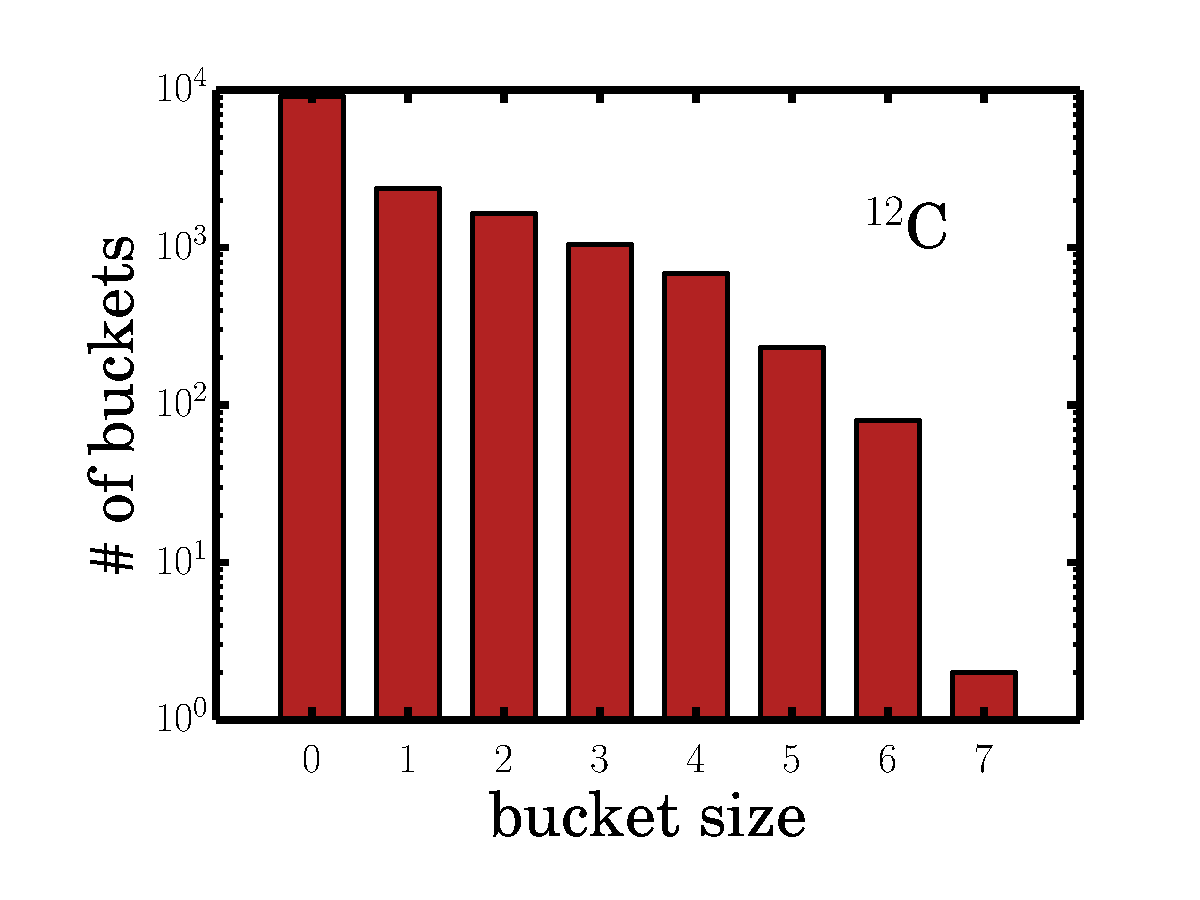
\includegraphics[width=0.45\textwidth]{figures/threej_map_buckets_12C.pdf}
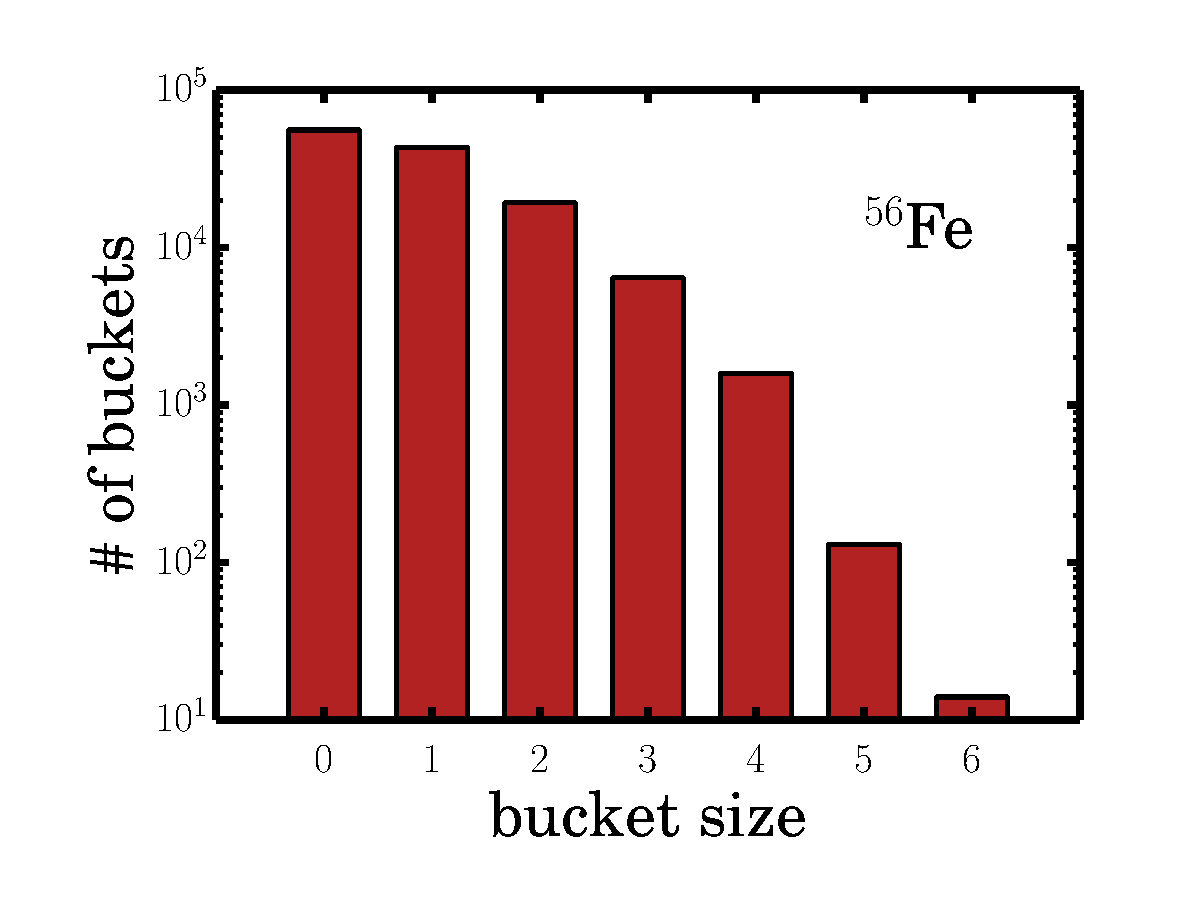
\includegraphics[width=0.45\textwidth]{figures/threej_map_buckets_56Fe.pdf}
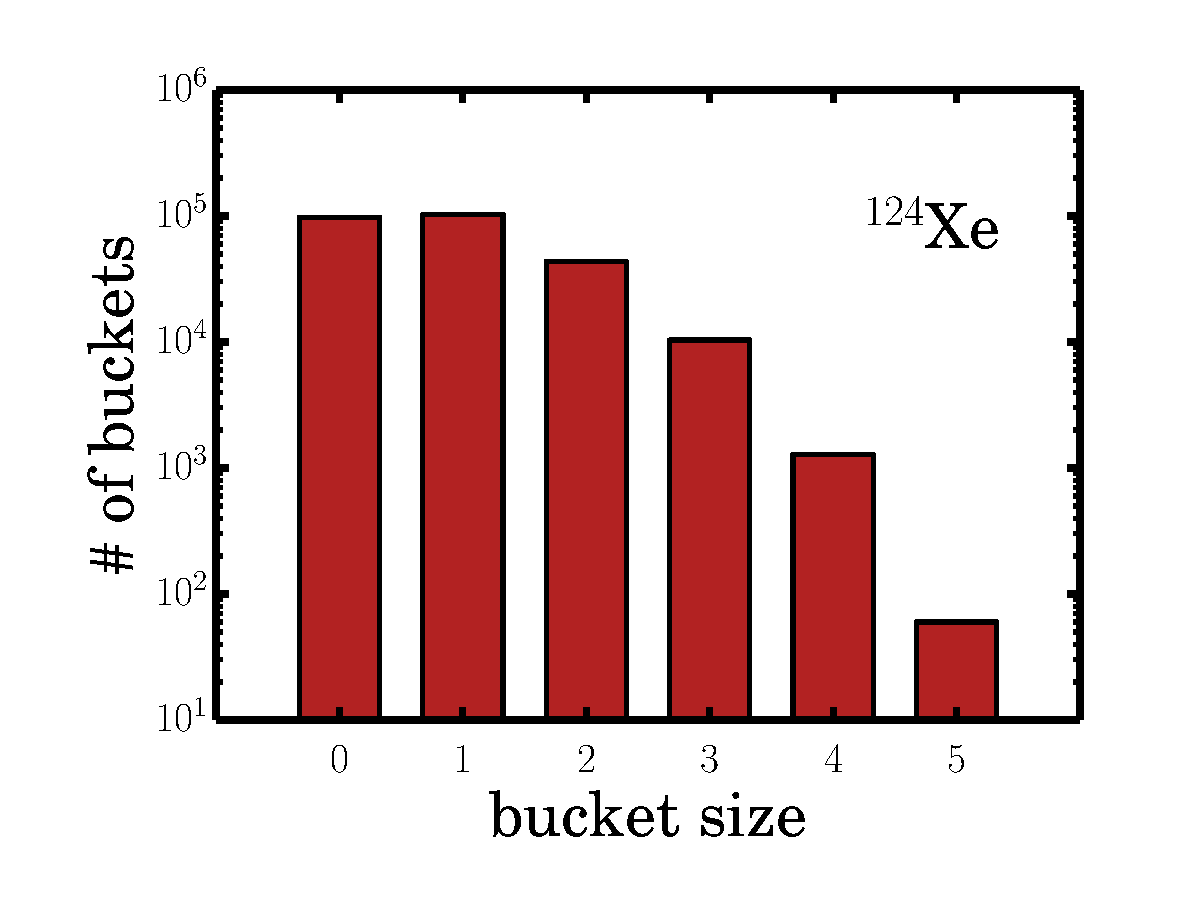
\includegraphics[width=0.45\textwidth]{figures/threej_map_buckets_124Xe.pdf}
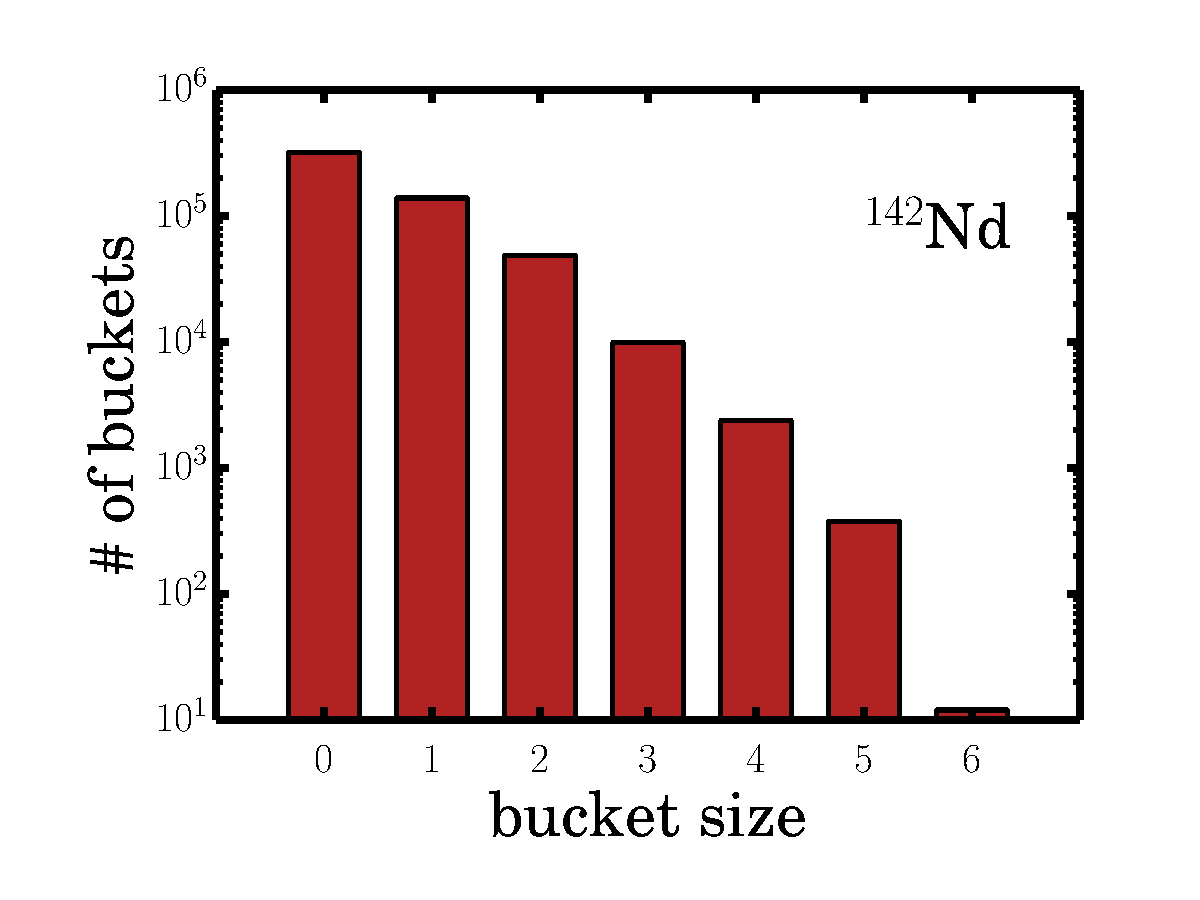
\includegraphics[width=0.45\textwidth]{figures/threej_map_buckets_142Nd.pdf}
\caption{An overview of the hash map ``buckets''. For $^{12}$C the collision rate is $80\%$, dropping to $60\%$ for $^{56}$Fe, $54\%$ for $^{124}$Xe and $50\%$ for $^{142}$Nd. Given that the collision rate drops when the mass number is increased, with the bucket sizes remaining small, combined with the fact that the number of buckets drops very fast for increasing bucket size, leads to the conclusion that the chosen hash key performs excellent.}
\end{figure}

\begin{figure}
\centering
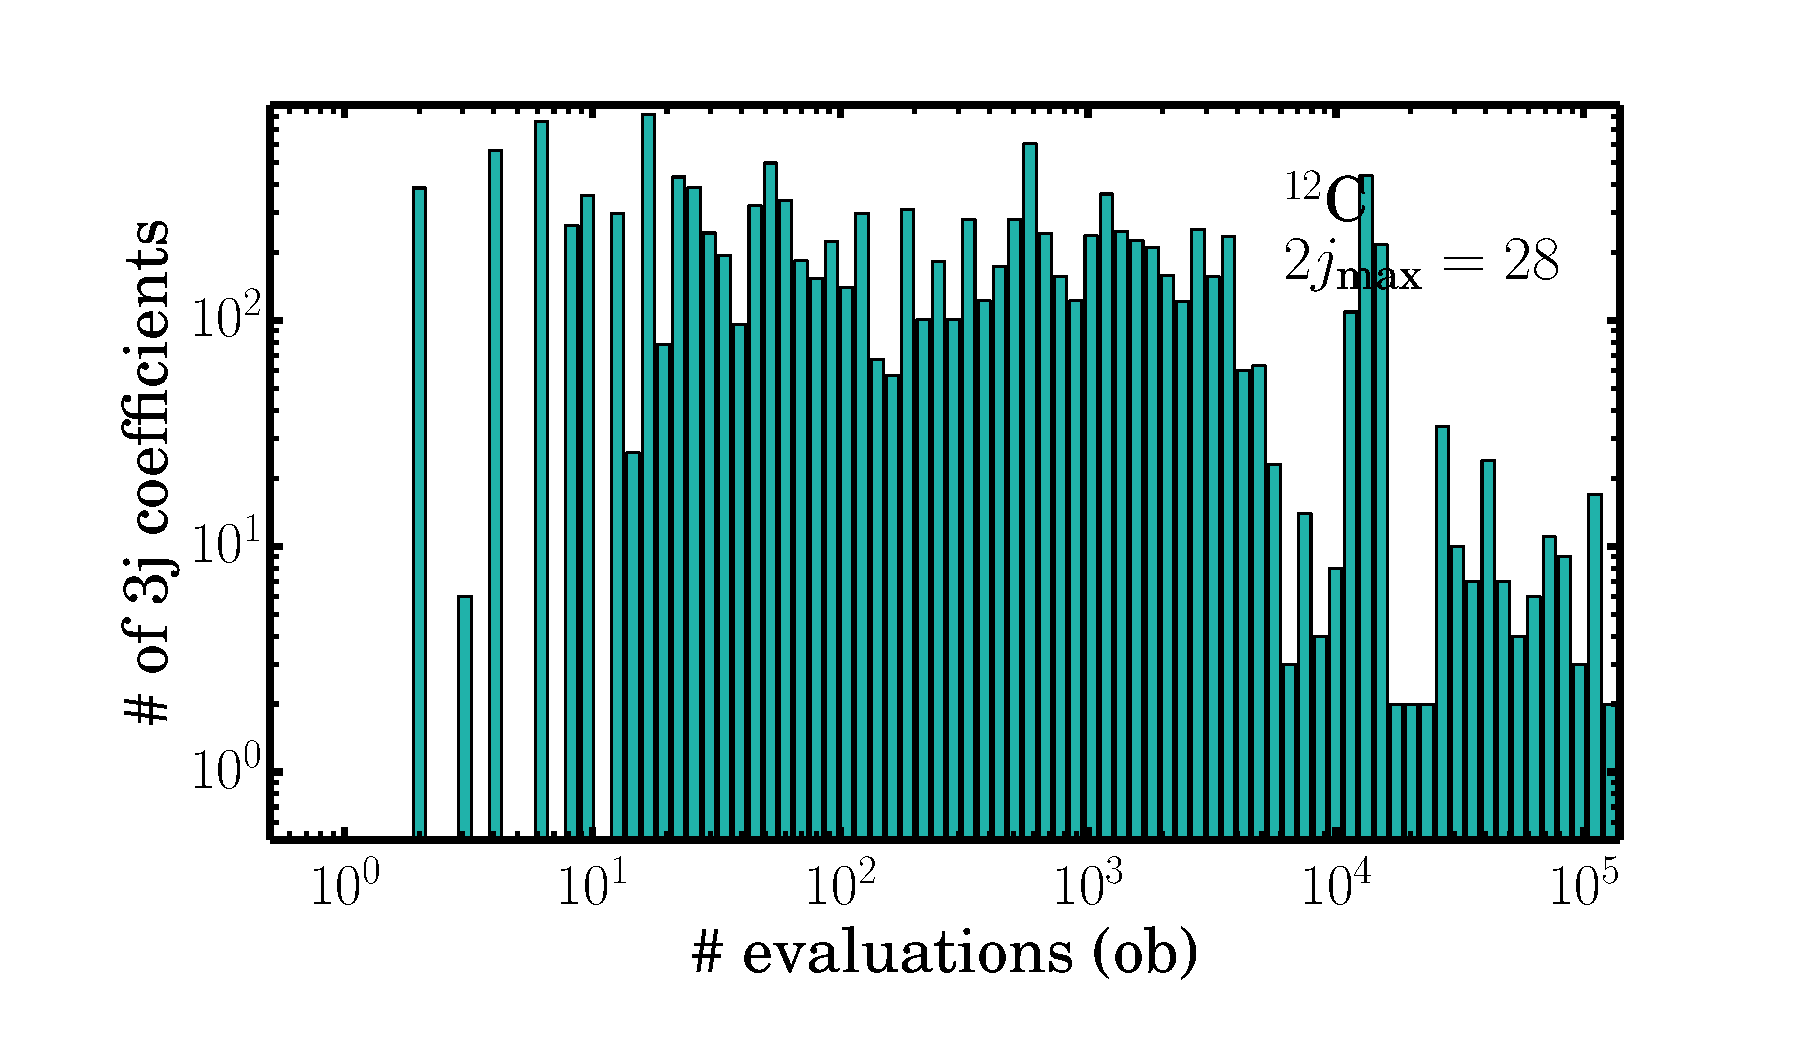
\includegraphics[width=\textwidth]{figures/threej_evals_12C.pdf}
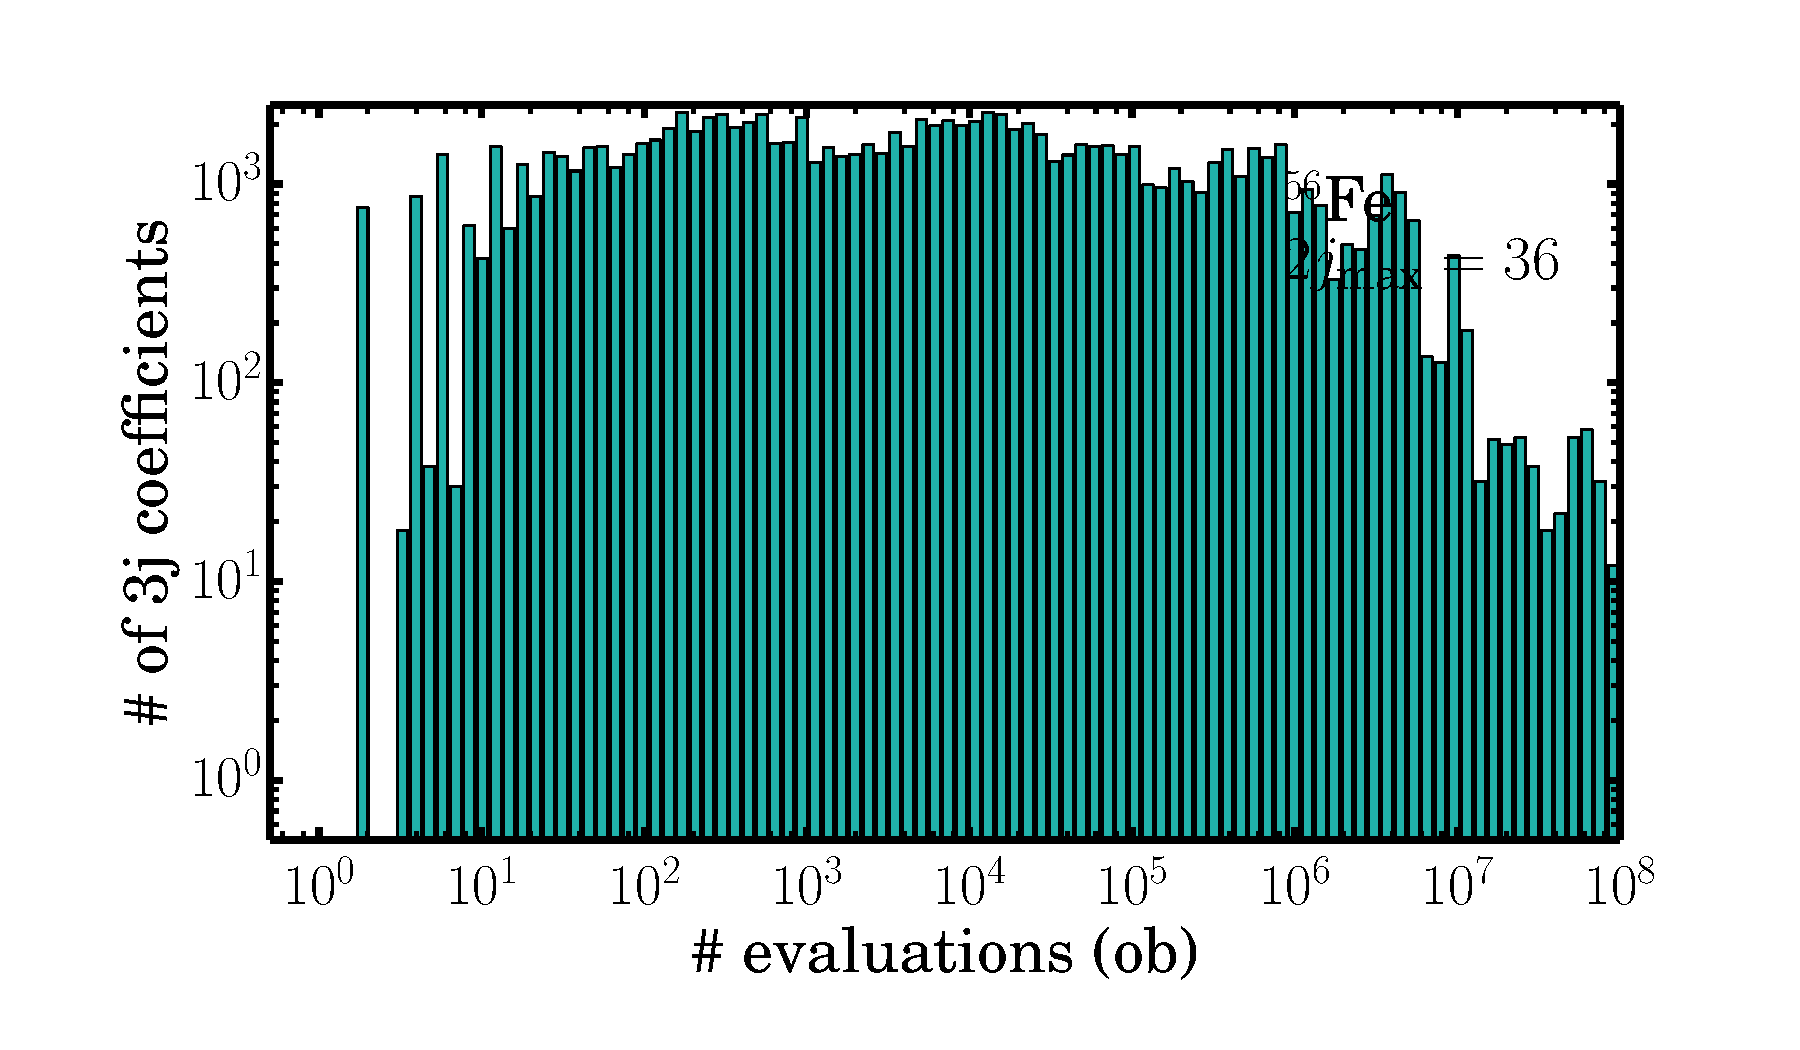
\includegraphics[width=\textwidth]{figures/threej_evals_56Fe.pdf}
\caption{The number of $3j$ coefficients in function of how many times they are evaluated. Note that both axes are logarithmic. For example, the first bar in both figures represent the number of $3j$ coefficients that have been evaluated twice.}
\end{figure}

\subsection{Heavy nuclei}

The one-body momentum distributions for heavy nuclei gets very noisy tails.
After extensive research it appeared that increasing integration precision
in \texttt{density\_ob\_integrand\_cf::calculate} softens this problem as shown in
figure~\ref{fig:ob_bad_tails}.

\todo[inline]{
The time the code takes to complete is dominated by the highest $l$-value
of the single-particle orbitals.
The main reason I have not yet been able to calculate $^{208}$Pb is because the 
valence shell has $l=6$ (for particle numbers above $112$).
$^{208}$Pb has 126 neutrons, meaning the $l=6$ is populated, and the computation time
is multiplied with a considerable factor. 
}

\begin{figure}
\centering
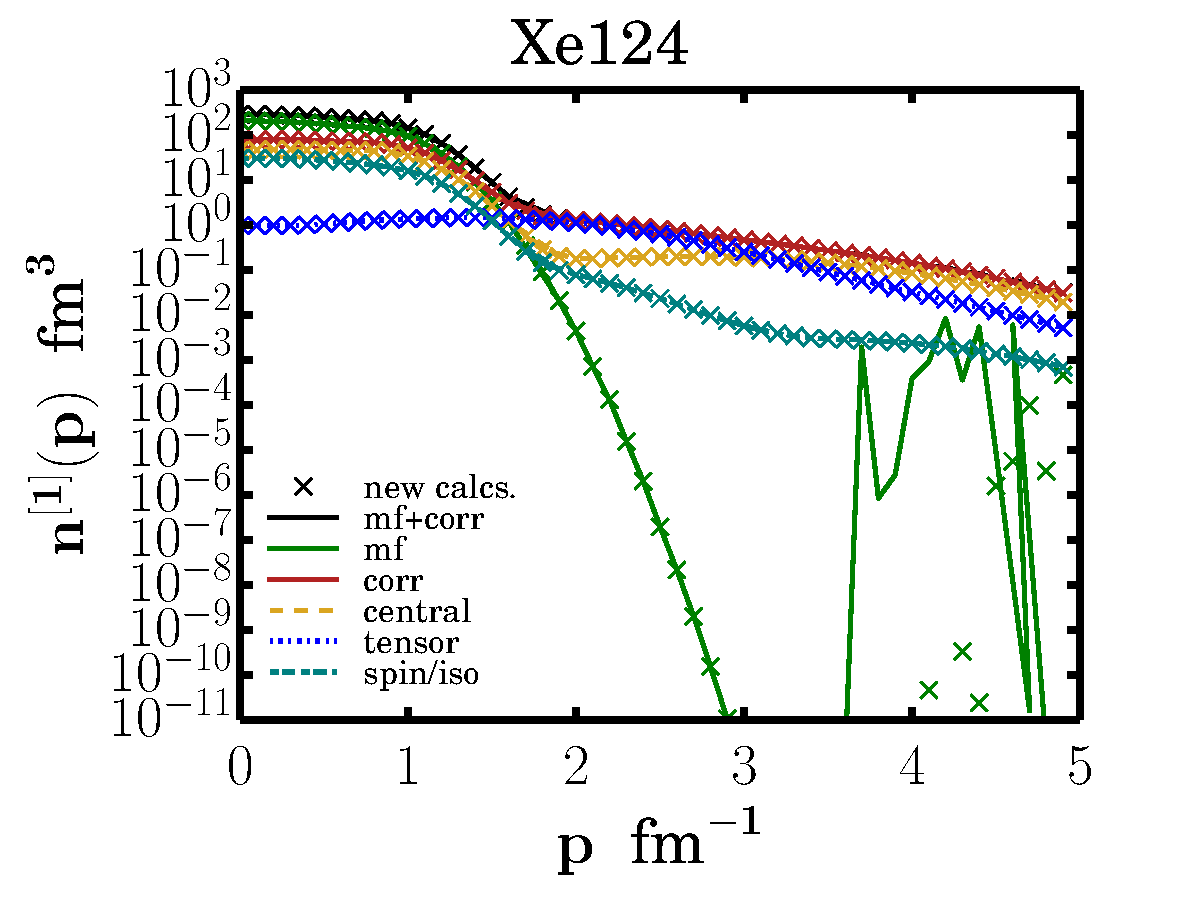
\includegraphics[width=0.7\textwidth]{figures/ob_Xe124_comparison.pdf}
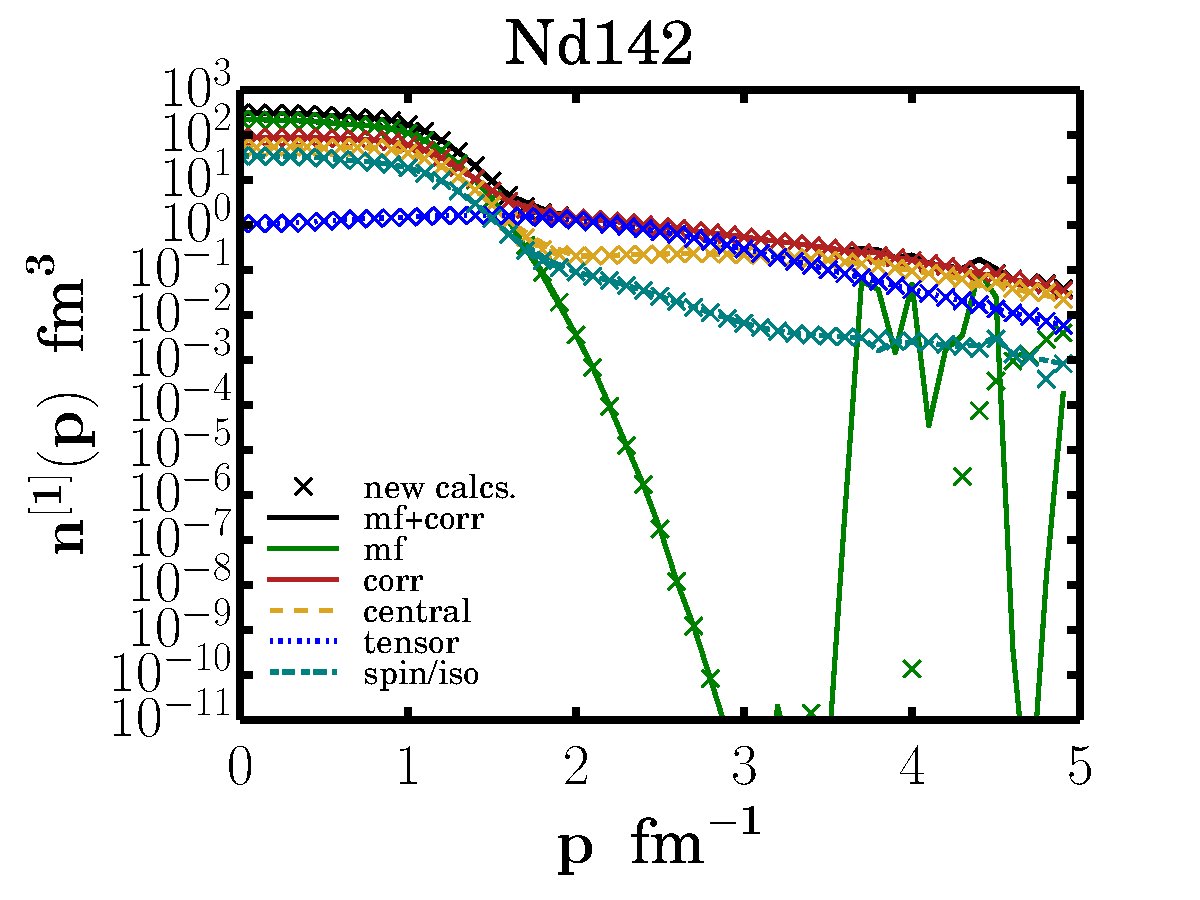
\includegraphics[width=0.7\textwidth]{figures/ob_Nd142_comparison.pdf}
\caption{The one-body momentum distribution before and after (new calcs.) the increased precision of \texttt{density\_ob\_integrand\_cf::calculate}.
The effect in $^{142}$Xe is almost invisible on the log scale but for $^{142}$Nd the fluctuations in
the tails become problematic. It is expected that this effect grows worse for increasing mass number $A$.}
\label{fig:ob_bad_tails}
\end{figure}

\begin{thebibliography}{10}

\bibitem{phdthesis_mvanhalst}
M.~Vanhalst
\newblock PhD thesis

\end{thebibliography}


\end{document}















%
%
%
%
% OBSOLOTE (WRONG) ISOSPIN PROJECTION THING
We now investigate the effect of the insertion of the isospin-projection operator $\hat{\delta}_{m_t}^{[i]}$ in 
\begin{align*}
	\braket{ T M_T | \hat{\vec{\tau}}_{1} \cdot \hat{\vec{\tau}}_{2} | T' M_T'}
\end{align*}
Note that $\hat{\delta}_{m_t}^{[i]}$ and $ \hat{\vec{\tau}}_{1} \cdot \hat{\vec{\tau}}_{2}$ are hermitian but do not commute. Hence the operator $\hat{\vec{\tau}}_{1} \cdot \hat{\vec{\tau}}_{2} \hat{\delta}_{m_t}^{[i]}$ is \textbf{not hermitian}.
\begin{align*}
	\hat{\vec{\tau}}_{1} \cdot \hat{\vec{\tau}}_{2} \hat{\delta}_{m_t}^{[1]} \ket { 1, \pm 1 } = \delta_{ \pm 1,2 m_t} \ket{ 1, \pm 1 }
\end{align*}
\begin{multline*}
	\hat{\vec{\tau}}_{1} \cdot \hat{\vec{\tau}}_{2} \hat{\delta}_{m_t}^{[1]} \ket { 1, 0 } = \frac{1}{\sqrt{2}} \Big( - \ket{ \frac{1}{2}, m_t} \otimes \ket{ \frac{1}{2}, -m_t} \\
	 + (1-2m_t) \ket{ \frac{1}{2}, m_t + 1} \otimes \ket{ \frac{1}{2},- m_t - 1} \\
	+  (1+2m_t) \ket{ \frac{1}{2}, m_t -1 } \otimes \ket{ \frac{1}{2}, -m_t + 1} \Big) \\
\end{multline*}
\begin{multline*}
	\hat{\vec{\tau}}_{1} \cdot \hat{\vec{\tau}}_{2} \hat{\delta}_{m_t}^{[1]} \ket { 0, 0 } = \frac{1}{\sqrt{2}} \Big( - 2m_t \ket{ \frac{1}{2}, m_t} \otimes \ket{ \frac{1}{2}, -m_t} \\
	 + (2m_t-1) \ket{ \frac{1}{2}, m_t + 1} \otimes \ket{ \frac{1}{2},- m_t - 1} \\
	+  (2m_t+1) \ket{ \frac{1}{2}, m_t -1 } \otimes \ket{ \frac{1}{2}, -m_t + 1} \Big) \\
\end{multline*}
The non-zero matrix elements for $ \braket{ T M_T | \hat{\vec{\tau}}_{1} \cdot \hat{\vec{\tau}}_{2} \hat{\delta}_{m_t}^{[i]} | T' M_T'}$ are (one can make use of the fact that both $\hat{\delta}_{m_t}^{[i]}$ and $ \hat{\vec{\tau}}_{1} \cdot \hat{\vec{\tau}}_{2}$ are hermitian and let them act on the neighbouring bra or ket),
\begin{multicols}{2}
\noindent
\begin{align*}
	\braket{ 1, \pm 1 | \hat{\vec{\tau}}_{1} \cdot \hat{\vec{\tau}}_{2} \hat{\delta}_{m_t}^{[1]} | 1, \pm 1} &= \delta_{ \pm 1,2m_t}  \\
	\braket{ 1,0 | \hat{\vec{\tau}}_{1} \cdot \hat{\vec{\tau}}_{2} \hat{\delta}_{m_t}^{[1]} | 1,0} &= \frac{1}{2} \\
	\braket{ 1,0 | \hat{\vec{\tau}}_{1} \cdot \hat{\vec{\tau}}_{2} \hat{\delta}_{m_t}^{[1]} | 0,0} &= \frac{1}{2}2m_t \\
	\braket{ 0,0 | \hat{\vec{\tau}}_{1} \cdot \hat{\vec{\tau}}_{2} \hat{\delta}_{m_t}^{[1]} | 1,0} &=-\frac{3}{2}2m_t \\
	\braket{ 0,0 | \hat{\vec{\tau}}_{1} \cdot \hat{\vec{\tau}}_{2} \hat{\delta}_{m_t}^{[1]} | 0,0} &=-\frac{3}{2}
\end{align*}
\begin{align*}
	\braket{ 1, \pm 1 | \hat{\vec{\tau}}_{1} \cdot \hat{\vec{\tau}}_{2} \hat{\delta}_{m_t}^{[2]} | 1, \pm 1} &= \delta_{ \pm 1,2m_t}  \\
	\braket{ 1,0 | \hat{\vec{\tau}}_{1} \cdot \hat{\vec{\tau}}_{2} \hat{\delta}_{m_t}^{[2]} | 1,0} &= \frac{1}{2} \\
	\braket{ 1,0 | \hat{\vec{\tau}}_{1} \cdot \hat{\vec{\tau}}_{2} \hat{\delta}_{m_t}^{[2]} | 0,0} &=-\frac{1}{2}2m_t \\
	\braket{ 0,0 | \hat{\vec{\tau}}_{1} \cdot \hat{\vec{\tau}}_{2} \hat{\delta}_{m_t}^{[2]} | 1,0} &= \frac{3}{2}2m_t \\
	\braket{ 0,0 | \hat{\vec{\tau}}_{1} \cdot \hat{\vec{\tau}}_{2} \hat{\delta}_{m_t}^{[2]} | 0,0} &=-\frac{3}{2}
\end{align*}
\end{multicols}
The non-zero matrix elements for $ \braket{ T M_T |  \hat{\delta}_{m_t}^{[i]} \hat{\vec{\tau}}_{1} \cdot \hat{\vec{\tau}}_{2} | T' M_T'}$ are,
\begin{multicols}{2}
\noindent
\begin{align*}
	\braket{ 1, \pm 1 | \hat{\delta}_{m_t}^{[1]} \hat{\vec{\tau}}_{1} \cdot \hat{\vec{\tau}}_{2} | 1, \pm 1} &= \delta_{ \pm 1,2m_t}  \\
	\braket{ 1,0 | \hat{\delta}_{m_t}^{[1]} \hat{\vec{\tau}}_{1} \cdot \hat{\vec{\tau}}_{2} | 1,0} &= \frac{1}{2} \\
	\braket{ 1,0 | \hat{\delta}_{m_t}^{[1]} \hat{\vec{\tau}}_{1} \cdot \hat{\vec{\tau}}_{2} | 0,0} &=-\frac{3}{2} 2m_t \\
	\braket{ 0,0 | \hat{\delta}_{m_t}^{[1]} \hat{\vec{\tau}}_{1} \cdot \hat{\vec{\tau}}_{2} | 1,0} &= \frac{1}{2} 2m_t \\
	\braket{ 0,0 | \hat{\delta}_{m_t}^{[1]} \hat{\vec{\tau}}_{1} \cdot \hat{\vec{\tau}}_{2} | 0,0} &=-\frac{3}{2}
\end{align*}
\begin{align*}
	\braket{ 1, \pm 1 | \hat{\delta}_{m_t}^{[2]} \hat{\vec{\tau}}_{1} \cdot \hat{\vec{\tau}}_{2} | 1, \pm 1} &= \delta_{ \pm 1,2m_t}  \\
	\braket{ 1,0 | \hat{\delta}_{m_t}^{[2]} \hat{\vec{\tau}}_{1} \cdot \hat{\vec{\tau}}_{2} | 1,0} &= \frac{1}{2} \\
	\braket{ 1,0 | \hat{\delta}_{m_t}^{[2]} \hat{\vec{\tau}}_{1} \cdot \hat{\vec{\tau}}_{2} | 0,0} &= \frac{3}{2} 2m_t \\
	\braket{ 0,0 | \hat{\delta}_{m_t}^{[2]} \hat{\vec{\tau}}_{1} \cdot \hat{\vec{\tau}}_{2} | 1,0} &=-\frac{1}{2} 2m_t \\
	\braket{ 0,0 | \hat{\delta}_{m_t}^{[2]} \hat{\vec{\tau}}_{1} \cdot \hat{\vec{\tau}}_{2} | 0,0} &=-\frac{3}{2}
\end{align*}
\end{multicols}

The non-zero matrix elements for $ \braket{ T M_T |  \hat{\delta}_{m_t}^{[i]} \hat{\vec{\tau}}_{1} \cdot \hat{\vec{\tau}}_{2} \hat{\delta}_{m_t}^{[i]} | T' M_T'}$ are,
\begin{align*}
	\braket{ 1, \pm 1 | \hat{\delta}_{m_t}^{[1]} \hat{\vec{\tau}}_{1} \cdot \hat{\vec{\tau}}_{2} \hat{\delta}_{m_t}^{[1]} | 1, \pm 1} &= \braket{ 1, \pm 1 | \hat{\delta}_{m_t}^{[2]} \hat{\vec{\tau}}_{1} \cdot \hat{\vec{\tau}}_{2} \hat{\delta}_{m_t}^{[2]} | 1, \pm 1} = \delta_{ \pm 1,2m_t}  \\
	\braket{ 1,0 | \hat{\delta}_{m_t}^{[1]} \hat{\vec{\tau}}_{1} \cdot \hat{\vec{\tau}}_{2} \hat{\delta}_{m_t}^{[1]} | 1,0} &= \braket{ 0,0 | \hat{\delta}_{m_t}^{[1]} \hat{\vec{\tau}}_{1} \cdot \hat{\vec{\tau}}_{2} \hat{\delta}_{m_t}^{[1]}| 0,0} = -\frac{1}{2} \\
	\braket{ 1,0 | \hat{\delta}_{m_t}^{[1]} \hat{\vec{\tau}}_{1} \cdot \hat{\vec{\tau}}_{2} \hat{\delta}_{m_t}^{[1]} | 0,0} &= \braket{ 0,0 | \hat{\delta}_{m_t}^{[1]} \hat{\vec{\tau}}_{1} \cdot \hat{\vec{\tau}}_{2} \hat{\delta}_{m_t}^{[1]}| 1,0}=-\frac{1}{2} 2m_t \\
		\braket{ 1,0 | \hat{\delta}_{m_t}^{[2]} \hat{\vec{\tau}}_{1} \cdot \hat{\vec{\tau}}_{2} \hat{\delta}_{m_t}^{[2]} | 1,0} &= \braket{ 0,0 | \hat{\delta}_{m_t}^{[2]} \hat{\vec{\tau}}_{1} \cdot \hat{\vec{\tau}}_{2} \hat{\delta}_{m_t}^{[2]}| 0,0} = -\frac{1}{2} \\
	\braket{ 1,0 | \hat{\delta}_{m_t}^{[2]} \hat{\vec{\tau}}_{1} \cdot \hat{\vec{\tau}}_{2} \hat{\delta}_{m_t}^{[2]} | 0,0} &= \braket{ 0,0 | \hat{\delta}_{m_t}^{[2]} \hat{\vec{\tau}}_{1} \cdot \hat{\vec{\tau}}_{2} \hat{\delta}_{m_t}^{[2]}| 1,0}=\frac{1}{2} 2m_t
\end{align*}
Note that the combinations of different isospin-projections are not necessarily zero when the operator $ \hat{\vec{\tau}}_{1} \cdot \hat{\vec{\tau}}_{2}$ is involved,
\begin{multicols}{2}
\noindent
\begin{align*}
	\braket{ 1,0 | \hat{\delta}_{m_t}^{[1]}  \hat{\vec{\tau}}_{1} \cdot \hat{\vec{\tau}}_{2} \hat{\delta}_{-m_t}^{[1]} | 1,0 } &= 1 \\
	\braket{ 1,0 | \hat{\delta}_{m_t}^{[1]}  \hat{\vec{\tau}}_{1} \cdot \hat{\vec{\tau}}_{2} \hat{\delta}_{-m_t}^{[1]} | 0,0 } &= -2m_t \\
	\braket{ 0,0 | \hat{\delta}_{m_t}^{[1]}  \hat{\vec{\tau}}_{1} \cdot \hat{\vec{\tau}}_{2} \hat{\delta}_{-m_t}^{[1]} | 1,0 } &= 2m_t \\
	\braket{ 0,0 | \hat{\delta}_{m_t}^{[1]}  \hat{\vec{\tau}}_{1} \cdot \hat{\vec{\tau}}_{2} \hat{\delta}_{-m_t}^{[1]} | 0,0 } &= -1
\end{align*}
\begin{align*}
	\braket{ 1,0 | \hat{\delta}_{m_t}^{[2]}  \hat{\vec{\tau}}_{1} \cdot \hat{\vec{\tau}}_{2} \hat{\delta}_{-m_t}^{[2]} | 1,0 } &= 1 \\
	\braket{ 1,0 | \hat{\delta}_{m_t}^{[2]}  \hat{\vec{\tau}}_{1} \cdot \hat{\vec{\tau}}_{2} \hat{\delta}_{-m_t}^{[2]} | 0,0 } &= 2m_t \\
	\braket{ 0,0 | \hat{\delta}_{m_t}^{[2]}  \hat{\vec{\tau}}_{1} \cdot \hat{\vec{\tau}}_{2} \hat{\delta}_{-m_t}^{[2]} | 1,0 } &=-2m_t \\
	\braket{ 0,0 | \hat{\delta}_{m_t}^{[2]}  \hat{\vec{\tau}}_{1} \cdot \hat{\vec{\tau}}_{2} \hat{\delta}_{-m_t}^{[2]} | 0,0 } &= -1
\end{align*}
\end{multicols}
These matrix element have been checked with a simple python program (\texttt{numpy.kron} ftw for kronecker products). Note that all the matrix elements for $i=1,2$ are the same expect for a minus sign whenever a combination like $ \braket{ 1,0 | \ldots | 0,0}$ or $\braket{0,0| \ldots | 1,0}$ is involved.
Also note that all the matrix elements do not mix different $M_T, M_T'$, so we effectively have $\delta_{M_T M_T'}$ everywhere.



